\chapter[CRYSTALLINE COHOMOLOGY, DIEUDONN\'E\hfill\break MODULES, AND JACOBI SUMS]{CRYSTALLINE COHOMOLOGY, DIEUDONN\'E MODULES, AND JACOBI SUMS}\label{art-6}

\begin{center}
{\large By~ Nicholoas M. Katz}
\end{center}

\setcounter{pageoriginal}{164}
\pageoriginale

%\tableofcontents


\section*{Introduction}
\pageoriginale
Hasse \cite{art6-key20} and Hasse-Davenport \cite{art6-key21} were the first to realize the connection between exponential sums over finite fields and the theory of zeta and $L$-functions of algebraic varieties over finite fields. This connection was exploited to Weil; one of the very first applications that Weil gave of the then newly proven ``Riemann Hypothesis'' for curves over finite fields was the estimation of the absolute value of Kloosterman sums (cf \cite{art6-key46}). The basic idea (cf \cite{art6-key20}) is that by using the theory of $L$-functions, one can express the negative of such an exponential sum as the sum of certain of the reciprocal zeroes of the zeta function itself; because the magnitude of these zeroes is given by the ``Riemann Hypothesis,'' one gets an estimate. In a fixed characteristic $p$, the estimate one gets in this way for all the fintie fields $\bF_{p^{n}}$ is best possible. On the other hand, very little is known about the variation with $p$ of the absolute values, even for Kloosterman sums, though in this case there is a conjecture, of Sato-Tate type, which seems inaccessible at present.

One case in which the problem of unknown variation with $p$ does not arise is when the expression of the exponential sum as a sum of reciprocal roots of zeta reduces to a sum consisting of a {\em single} reciprocal root; then the Riemann Hypothesis tells us the exact magnitude of the exponential sum. Conversely, an elementary argument shows that in a certain sense, this is the only case in which such exact knowledge of the magnitude of exponential sums can arise, and it shows further that a theorem of Hasse-Davenport type always results from such exact knowledge. Examples of exponential sums of this sort are Gauss sums and Jacobi sums.

Honda was the first to suggest that the identification of say, Jaboci sums, with reciprocal zeroes of zeta functions could also lead to significant non-archimedean information about Jacobi sums. A few years before his untimely death, Honda conjectured a $p$-adic limit formula for Jacobi sums in terms of ratios of binomail coefficients (\cite{art6-key23}). I gave an over-complicated proof (in a letter to Honda of Nov. 1971) which managed to shed no light whatever on the meaning of the formula. Recently, B. H. Gross and N. Koblitz \cite{art6-key14} showed that Honda's limit formula was really an {\em exact} $p$-adic formula for Jacobi sums in terms of products of values of Morita's $p$-adic $\Gamma$-function; as such, it constituted the first improvement in this century over Stickelberger's formula which gave the $p$-adic\pageoriginale valuation and the {\em first} non-vanishing $p$-adic digit in the $p$-adic expansion of a Jacobi sum!

In this paper, I will discuss the cohomological genesis of formulas of the sort discovered by Honda. The basic idea is that the reciprocal zeroes of zeta are the eigenvalues of the Frobenius endomorphism of a suitable cohomology group; if this group, together with the action of Frobenius upon it, can be made sufficiently explicit, one obtains the desired ``explicit formulas''.

There are two approaches to the question, which differ more in style than in substance. The first and longer is based on Honda's explicit construction of the Dieudonn\'e module of a formal group in terms of ``formal de Rham cohomology''. The second, less elementary but more efficient, is grounded in crystalline cohomology, particularly in the theory of the de Rham-Witt complex. I hope the reader will share my belief that there is something to be gained from each of the approaches, and pardon my decision to discuss both of them.

I would like to thank B. Dwork for many helpful discussions concerning the original proof of Honda's conjecture. Whatever I know of the Grothendieck-Mazur-Messing approach to Dieudonn\'e theory\break through exotic Ext's, I was taught by Bill Messing. I would also like to thank Spencer Bloch for his encouragement when I was trying to understand Honda's explicit Dieudonn\'e theory, and Luc Illusie for gently correcting some extravagent assertions I made at the Colloquium.

Finally, I would like to dedicate this paper to the memory of T. Honda.

\medskip
\noindent
{\bf I. Elementary Axiomatics, and the Hasse-Davenport Theorem.}
Consider a projective, smooth and geometrically connected variety $X$, say of dimension $d$, over a finite field $\bF_{q}$. For each integer $n\geq 1$, we denote by $X(\bF_{q^{n}})$ the finite set of points of $X$ with values in $\bF_{q^{n}}$, and by $\sharp X(\bF_{q^{n}})$ the cardinality of this set. The zeta function $Z(X/\bF_{q},T)$ of $X$ over $\bF_{q}$ is the formal power series in $T$ with $Q$-coefficients defined as
$$
Z(X/\bF_{q},T)=\exp \left(\sum\limits_{n\geq 1}\frac{T^{n}}{n}\sharp X(\bF_{q^{n}})\right).
$$
Thanks\pageoriginale to Deligne \cite{art6-key6}, we know that this zeta function has a unique expression as a finite alternating product of polynomials $P_i (T) \in \bZ [T]$, $i = 0, \ldots, 2d$:
$$
Z (X/ \bF_q, T) = \prod\limits^{2d}_{i=0} P_i (T)^{(-1)^{i+1}} = \frac{P_1 P_3 \ldots P_{2d-1}}{P_0 P_2 \ldots P_{2s}}
$$
in which each polynomial $P_i (T) \in\bZ[T]$ is of the form 
$$
P_i (T) = \prod\limits^{\deg P_i}_{j=1} (1 -\alpha_{i,j} T)
$$
with $\alpha_{i,j}$ algebraic integers such that 
$$
|\alpha_{i,j}| = \sqrt{q}^i
$$
for \textit{any} archimedean absolute value $|\;|$ on the field $\bar{\bQ}$ of all algebraic numbers. The extreme polynomials $P_0$, $P_{2d}$ are given explicitly:
$$
P_0 (T) = (1-T) , P_{2d} (T) = (1 - q^d \cdot T)
$$

Despite this apparently ``elementary'' characterization of the polynomials $P_i (T)$, their true genesis is cohomological. Let us recall this briefly.

For each prime number $l$ different from the characteristic $p$ of $\bF_q$, let us denote by $H^i_l(X)$ the finitely generated $\bZ_l$-module defined as 
$$
H^i_l (X) =  \varprojlim_n H^i_{\text{etale}} (X \otimes \bar{\bF}_q, \bZ / l^n \bZ ).
$$
Corresponding to the prime $p$ itself, we denote by $W(\bF_q)$ the ring of $p$-Witt vectors of $\bF_q$, and by $H^i_{\text{cris}} (X)$ the finitely generated $W(\bF_q)$-module defined as 
$$
H^i_{\text{cris}} (X) = \varprojlim_n H^i_{\text{cris}} (X / W_n (\bF_q)).
$$
The Frobenius endomorphism $F$ of $X$ relative to $\bF_q$ acts, by functoriality, on these various cohomology groups $H^i_l(X)$ for $l\neq p$, and $H^i_{\text{cris}} (X)$; and $F$ induces automorphisms of the corresponding vector spaces 
$$
H^i_l(X) \bigotimes_{Z_l} Q_l, \ H^i_{\text{cris}} (X) \bigotimes_{W(\bF_q)} K
$$ 
($K$ denoting the fraction field of $W(\bF_q)$). The polynomial $P_i (T) \in \bZ [T]$ which occurs in the factorization of the zeta function is then given cohomologically by the formulas 
\begin{gather*}
P_i(T) = \det (1 - T F \big| H^i_l(X) \otimes \bQ_l) \text{ for } l \neq p\\
P_i (T) = \det (1 - T F \big| H^i_{\text{cris}} (X) \otimes K).
\end{gather*}\pageoriginale 

The resulting formula for zeta as the alternating product of characteristic polynomials of $F$ on the $H^i$, in each of the cohomology theories $H^i_l (X) \otimes Q_l$ for $l \neq p$, $H^i_{\text{cris}} (X) \otimes K$, is equivalent, via logarithmic differentiation, to the identities in those theories 
$$
\neq X (\bF_{q^n}) = \sum (-1)^i \text{ trace } (F^n \big| H^i). \text{ for all } n \geq 1.
$$
By viewing the set $X(\bF_{q^n})$ as the set of fixed points of $F^n$ acting on $X(\bar{\bF}_q)$, this identity becomes a Lefschetz trace formula
$$
\# \text{ Fix } (F^n ) =\sum(-1)^i \text{ trace } (F^n \big| H^i) \text{ all } n \geq 1
$$
for $F$ and its iterates in each of our cohomology theories. If we take as \textit{given} these Lefschetz trace formulas, then the identification of $P_i$ with $\det (1 - F T \big| H^i)$ is equivalent to the assertion:
\begin{align*}
&\text{On any of the groups $H^i_l(X) \otimes Q_l$ with $l \neq p$,}\\
&\text{$H^i_{\text{cris}} (X) \otimes K$, the eigenvalues of $F$ are alge-}\\
&\text{braic integers all of whose archimedean absolute}\\
&\text{values are $\sqrt{q}^i$.}
\end{align*}
In fact, there is not a great deal more that is known about the action of $F$ on the $H^i_l(X) \otimes Q_l$ for $l \neq p$, and on $H^i_{\text{cris}} (X)  \otimes K$. It is still \textit{not} known, for example, whether the action of $F$ on these cohomology groups is always semi-simple when $i>1$. (That it is when $i =1$ results from the theory of abelian varieties).

Suppose that a finite group $G$ operates on $X$ by $\bF_q$-automorphisms. Let us choose a number field $E$ big enough that all complex representations of $G$ are realizable over $E$, and whose residue fields at all $p$-adic places contain $\bF_q$. (For example, the field $Q(\zeta_{q-1}, \zeta_N)$, where $N$ is the $l$.c.m. of the orders of elements of $G$, is such an $E$). We denote by $\lambda$ an $l$-adic place of $E$, $l \neq p$, and by $\sfP$ a $p$-adic place of $E$. Thus $E_\lambda$ is a finite extension of $Q_l$, and $E_\sfP$ is a finite extension of $K$.

Let $M$ be a finite dimensional $E$-vector space given with an action of $G$, say $\rho : G \to \Aut_E (M)$. The associated $L$-function $L(X/\sF_q, \rho, T)$ is the formal power series with $E$-coefficients defined as 
$$
L(X/\sF_q, \rho, T) = \exp \left(\sum\limits_{n \geq 1} \frac{T^n}{n} \cdot \frac{1}{\# G} \sum\limits_{g \in G} tr (\rho (g^{-1})) \# Fix (F^n g) \right)
$$\pageoriginale
where Fix $(F^n g)$ denotes the finite set of fixed points of $F^ng$ acting on $X(\bar{\bF}_q)$. We recover the zeta function of $X/\bF_q$ by taking for $\rho$ the regular representation of $G$. The usual formalism of zeta and $L$-functions gives 
$$
Z(X/ \bF_q, T) = \prod\limits_{\rho \text{ irred}} L (X / \bF_q, \rho, T)^{\deg (\rho)}
$$

It follows from Deligne's results that for any representation $\rho$, we have a unique expression for the corresponding $L$-function as an alternating product of polynomials $P_{i,\rho}(T) \in E [T]$,
$$
L(X/ \bF_{q}, \rho, T) =\prod\limits^{2d}_{i=0} P_{i,\rho} (T)^{(-1)^{i+1}},
$$
which are of the form 
$$
P_{i,\rho} (T) = \prod\limits^{\deg P_{i,\rho}}_{j=1} (1 - \alpha_{i, j, \rho} T)
$$
with algebraic integers $\alpha_{i, j,\rho}$ such that 
$$
|\alpha_{i, j, \rho}| = \sqrt{q}^i
$$
for any archimedean absolute value $|\;|$ on the field $\bar{Q}$ of all algebraic numbers. 

The cohomological expression of there $P_{i,\rho}$ is straighforward\break  (\cf\cite{art6-key18}). Because the action of $G$ is ``defined over $\bF_q$'' it commutes with $F$, and therefore the induced action of $G$ on the cohomology commutes with the action of $F$. Therefore $G$, acting by composition, induces automorphisms of the $E_\lambda$-vector spaces,$l \neq \rho$,
$$
\Hom_{E_\lambda [G]} (M\bigotimes\limits_E E_\lambda, H^i_l (X) \bigotimes\limits_{Z_l} E_\lambda).
$$
and of the $E_\sfP$-vector spaces
$$
\Hom_{E_{\sfP} [G]} (M \bigotimes\limits_{E} E_\sfP, H^i_{\text{cris}} (X) \bigotimes\limits_{W(\sF_q)} E_\sfP). 
$$
The polynomials $P_{i, \rho} (T) \in E [T]$ are given by the formulas 
\begin{align*}
P_{i,\rho} (T) & = \det (1 - T F \big| \Hom_{E_\lambda [G]} (M \bigotimes\limits_{E} E_\lambda, H^i_l (X) \bigotimes\limits_{Z_l} E_\lambda )) \text{ for } l \neq \rho \\
P_{i, \rho} (T) & = \det (1 - TF \big| \Hom_{E_\sfP [G]} (M\bigotimes\limits_E E_\sfP, H^i_{\text{cris}} (X) \bigotimes\limits_{W (\sF_q)} E_\sfP)).
\end{align*}

Let us\pageoriginale recall the derivation of these formulas. We first observe that the characteristic polynomial of $F$ on $\Hom_G (M, H^i) \simeq ({\displaystyle{\mathop{M}^v}} \otimes H^i)^G \subset {\displaystyle{\mathop{M}^v}} \otimes H^i$ \textit{divides} $\det (1-F T \big| H^i)^{\dim {\displaystyle{\mathop{M}^v}}}$, and hence the eigenvalues of $F$ on $\Hom_G (M, H^i)$ are algebraic integers, all of whose archimedean absolute values are $\sqrt{q}^i$. So it remains only to verify that the alternating product of those characteristic polynomials is indeed the $L$-function, \ie. that 
$$
L(X \backslash \bF_q, \rho, T) = \prod \det (1 - F T \big| ({\displaystyle{\mathop{M}^v}} \otimes H^i)^{G} )^{(-1)^{i+1} },
$$
Equivalently, we must check that 
\begin{align*}
\frac{1}{\# G} \sum \text{ trace }\rho  (g^{-1}) &\;\# \text{ Fix } (F^n g)\\
& = \sum (-1)^i \text{ trace } (1 \otimes F^n \big| ({\displaystyle{\mathop{M}^v}} \otimes H^i)^G)\\
& = \sum (-1)^i \frac{1}{\# G} \sum\limits_{g \in G} \text{ trace } (g \otimes F^n g \big|{\displaystyle{\mathop{M}^v}} \otimes H^i)\\
& = \sum (-1)^{i} \frac{1}{\# G} \sum\limits_{g \in G} \text{ trace } {\displaystyle{\mathop{\rho}^v}} (g) \cdot \text{ trace } (F^n g \big| H^i)\\
& = \frac{1}{\# G} \sum\limits_{g \in G}  \text{ trace } \rho (g^{-1}) \sum (-1)^i \text{ trace } (F^n g \big| H^i). 
\end{align*}
To check this last equality, we would like to invoke the Lefschetz trace formula, not for $F^n$, but for $F^ng$, with $g$ an automorphism of \textit{finite order} which commutes with $F$; this amounts to invoking the Lefschetz trace formula for $Fg$ on $X$ and on all its ``extensions of scalars'' $X \otimes \bF_{q^n}$. But an elementary descent argument shows that given an automorphism $g$ of finite order which commutes with $F$, there is \textit{another} variety $X'/ \bF_q$ together with an isomorphism $X \otimes \bar{\bF}_q \simeq X' \otimes \bar{\bF}_q$ under which $F g \otimes 1$ corresponds to $F \otimes 1$. Because this isomorphism also induces isomorphisms of cohomology groups 
\begin{gather*}
H^i_l (X)^{\text{dfn}} H^i_{\text{et}} (X' \otimes \bar{\bF}_q, \bZ_l) \simeq H^i (X \otimes \bar{\bF}_q, \bZ_l)^{\text{dfn}} H^i_l(X),\\
H^i_{\text{cris}} (X') \otimes W (\bar{\bF}_q) \simeq H^i_{\text{cris}} (X' \otimes \bar{\bF}_q) \simeq H^i_{\text{cris}} (X \otimes \bar{\bF}_q) \simeq\\
\simeq H^i_{\text{cris}} (X) \otimes W (\bar{\bF}_q),
\end{gather*}
the truth\pageoriginale of the Lefschetz formula for $Fg$ on $X$ results from its truth for $F$ on $X'$.

Let us now consider in greater detail the case of an irreducible $\rho$. Then $P_{i, \rho}$ is a polynomial whose degree is the common \textit{multiplicity} of $\rho$ in any of the $H^i_l(X) \otimes E_\lambda$, $l \neq \rho$, or in $H^i_{\text{cris}} (X) \otimes E_\sfP$. Decomposing the regular representation leads to the factorization
$$
P_i (T) = \prod\limits_{\rho \text{ irred}} P_{i, \rho} (T)^{\deg (\rho)}
$$
The coarser factorization 
$$
P_i (T) = \prod\limits_{ \rho \text{irred}} (P_{i,\rho} (T)^{\deg(\rho)})
$$
corresponds to the decomposition of $H^i_l(X) \otimes E_\lambda$, $\resp H^i_{\text{cris}} (X) \otimes E_\sfP$, into $\rho$-isotypical components
\begin{gather*}
H^i_l (X) \otimes E_\lambda \simeq \bigotimes\limits_{\text{irred} \rho } \left(H^i_l(X) \times E_\lambda \right)^\rho\\
H^i_{\text{cris}} (X) \otimes E_\sfP \simeq \bigotimes\limits_{\text{irred} \rho} \left(H^i_{\text{cris}} (X) \otimes E_\sfP \right)^\rho
\end{gather*}
Indeed the corresponding identities, for $\rho$ irreducible, are 
\begin{align*}
P_{i,\rho} (T)^{\deg(\rho)}  & = \det (1 - TF \big| (H^i_l (X) \otimes E_\lambda)^\rho) l \neq p\\
P_{i, \rho} (T)^{\deg (\rho)} & = \det (1 - TF \big| (H^i_{\text{cris}} (X) \otimes E_\sfP)^\rho).
\end{align*}

Let us denote by $S(X/ \bF_q, \rho, n)$ the exponential sums used to define the $L$-function:
$$
S (X/ \sF_q , \rho, n) = \frac{1}{\# G} \sum\limits_{g \in G} tr (\rho (g)) \# \text{ Fix }(F^n g^{-1}). 
$$
The following lemma gives the cohomological meaning of theorems of Hasse-Davenport type (\cf \cite{art6-key20}).

\medskip
\noindent
{\bfseries Lemma \thnum{1.1}:\label{art6-lem1.1}}
\textit{Let $X/\bF_q$ be projective and smooth. Let a finite group $G$ operate on $X$ by $\bF_q$-automorphisms, and let $p$ be an irreducible complex representation of $G$. Fix an integer $i_\circ$, and denote by $H^{i_\circ}$ any one of the cohomology groups $H^{i_\circ}_l(X) \bigotimes_{Z_l} E_\lambda$ with $l \neq p$, or $H^{i_\circ}_{\text{cris}}(X) \bigotimes\limits_{W(\bF_q)} E_\sfP$. Let $|\;|$ be any archimedean absolute value on the filed $\bar{Q}$ of all algebraic numbers. The following conditions are equivalent:}
\begin{enumerate}
\item[(1)] \textit{The\pageoriginale multiplicity of $\rho$ in $H^{i_\circ}$ is one, and the multiplicity of $\rho$ in $H^i$ is zero if $i \neq i_\circ$.}

\item[(2)] \textit{For all $n \geq 1$, we have }
\begin{gather*}
(-1)^{i_\circ} S (X / \bF_q, \rho,n) = ((-1)^{i_\circ} S (X / \bF_q, \rho, 1))^n,\\
\text{and } \hspace{3cm}|S (X / \bF_q, \rho, 1)| = \sqrt{q}^{i_\circ} \hspace{3cm}
\end{gather*}

\item[(3)] \textit{For all $n \geq 1$, we have}
$$
|S(X/ \bF_q, \rho, n)| = \sqrt{q}^{i_\circ n}
$$

\item[(4)] \textit{For all $n \geq 1$, we have }
\begin{gather*}
|S (X/ \bF_q, \rho, n)| = |S(X/ \bF_q,  \rho, 1)|^n\\
\text{and } \hspace{3cm} \sqrt{q}^{i_\circ} \leq |S (X / \bF_q, \rho, 1)| < \sqrt{q}^{1+ i_\circ}\hspace{3cm}
\end{gather*}

\item[(5)] \textit{The polynomial $P_{i_{\circ, \rho}} (T)$ is given by}
$$
P_{i_{\circ, \rho}} (T) = 1 - (-1)^{i_\circ} S (X / \bF_q, \rho, 1) T 
$$
\textit{and for $i \neq i_\circ$, we have $P_{i,\rho} (T) =1$.}

\item[(6)] \textit{The $\rho$-isotypical component $(H^i)^\rho =0$ for $i \neq i_\circ$, $(H^{i_\circ})^\rho$ has dimension $ = \deg (\rho)$, and $F$ operates on $(H^{i_\circ})^\rho$ as the scalar 
$$
(-1)^{i_\circ} S (X/ \bF_q, \rho, 1).
$$}
\end{enumerate}

\begin{proof}
This is an easy exercise, using the basic identities:
$$
\left\{
\begin{aligned}
&\exp \left(\sum \frac{T^n}{n}  S (X / \bF_q, \rho, n)\right) = L (X/ \bF_q, \rho, T) = \prod\limits_{i} P_{i,\rho} (T)^{(-1)^{i+1}}\\
& \quad P_{i,\rho} (T) = \prod\limits_j (1 - \alpha_{i,j,\rho} T), |\alpha_{i,j,\rho}| = \sqrt{q}^i\\
& \deg P_{i,\rho} = \textit{ multiplicity of $\rho$ in } H^i = \frac{1}{\deg (\rho)} \cdot \dim ((H^i)\rho).
\end{aligned}
\right.
$$

Suppose, first, that (1) holds, or equivalently that for $i \neq i_\circ$, $P_{i,\rho} (T) =1$, while $P_{i_{\circ, \rho}}$ is a linear polynomial $P_{i_{\circ,\rho}} (T) = (1-A T)$ with $|A| = \sqrt{q}^{i_\circ}$. The cohomological expression for $L$ then becomes 
$$
\exp \left(\sum \frac{T^n}{n} S (X/ \bF_q, \rho, n) \right) = \left(\frac{1}{1-AT} \right)^{(-1)^{i_\circ}}.
$$
Taking\pageoriginale logarithms and equating coefficients, we find 
$$
(-1)^{i_\circ} S (X/ \bF_q, \rho, n) = A^n \quad \text{ for all } n \geq 1. 
$$
 
In particular (2) and (5) hold.

The implications (5) $\Rightarrow$ (1), (6) $\Rightarrow$ (1) are obvious. Also (5) $\Rightarrow$ (6), for if $P_{i_{\circ, \rho}}$ is linear, then $\rho$ has multiplicity one in $H^{i_\circ}$, so that $(H^{i_\circ})^\rho$ is $G$-irreducible, and hence $F$ must operate on $(H^{i_\circ})^\rho$ as a \textit{scalar}, which we compute by the formula
$$
P_{i_{\circ, \rho}} (T)^{\deg (\rho)} = \det (1 - TF \big| (H^{i_\circ})^\rho).
$$

Clearly we have (2) $\Rightarrow$ (3) $\Rightarrow$ (4). We must show that if (4) holds, then exactly \textit{one} of the $P_{i,\rho}$ is $\neq 1$, and that one is linear. Logarithmically differentiating the cohomological formula for $L$, we find 
$$
S(X/ \bF_q, \rho, n) = \sum\limits_i (-1)^i \sum\limits^{\deg P_{i, \rho}}_{j=1} (\alpha_{i, j, \rho})^n, \quad |\alpha_{i,j,\rho}| = \sqrt{q}^i.
$$
We must show that if (4) holds, then the double sum has only a single term in it. Separating the $\alpha_{i, j, \rho}$ according to the \textit{parity} of $i$, we get two disjoint sets of non-zero complex numbers (disjoint because their absolute values are disjoint), to which we apply the following lemma.
\end{proof}

\medskip
\noindent
{\bfseries Lemma \thnum{1.2}:\label{art6-lem1.2}}~{\em Let $N\geq 0$ and $M\geq 0$ be non-negative integers. Let $\{A_{i}\}$ be a family of $N$ not-necessarily distinct elements of $C^{x}$, and $\{B_{i}\}$ a family of $M$ not-necessarily distinct elements of $C^{x}$. Suppose that for all $i$, $j$, $A_{i}\neq B_{j}$. If, for some real number $R>0$, we have}
$$
\left| \sum A^{n}_{j}-\sum B^{n}_{j}\right|=R^{n}\quad \text{\em for all $n\geq 1$,}
$$
{\em then $N+M=1$, i.e. either there is just one $A$ and no $B$'s, or just one $B$ and no $A$'s.}
\smallskip

\begin{proof}
Suppose first that either $N=0$ or $M=0$, say $M=0$. Then we have
$$
\left| \sum A^{n}_{i}\right|=R^{n}.
$$
Squaring, we get
$$
\sum\limits_{ij}(A_{i}\overline{A}_{j})^{n}=(R^{2})^{n}\quad\text{for}\quad n\geq 1
$$
whence\pageoriginale
$$
\prod\limits_{ij}(1-A_{i}\overline{A}_{j}T)=(1-R^{2}T),
$$
and hence $N=1$.

In case both $N\geq 1$ and $M\geq 1$, squaring leads to
$$
\sum (A_{i}\overline{A}_{k})^{n}+\sum(B_{j}\overline{B}_{l})^{n}=(R^{2})^{n}+\sum(A_{i}\overline{B}_{j})^{n}+\sum (\overline{A}_{i}B_{j})^{n}
$$
or equivalently,
$$
\frac{1}{(1-R^{2}T)}=\frac{\prod (1-A_{i}\overline{B}_{j}T)\prod(1-\overline{A}_{i}B_{j}T)}{\prod(1-A_{i}\overline{A}_{k}T)\prod(1-B_{j}\overline{B}_{l}T)}
$$
Let $R_{\max}$ be $\max (|A_{i}|,|B_{j}|)$, and consider the order of pole at $T=R^{-2}_{\max}$. The numerator's factors $1-A_{i}\overline{B}_{j}T$, $1-\overline{A}_{i}B_{j}T$ are all non-zero there (for if $A_{i}\overline{B}_{j}=R^{2}_{\max}$, by maximality we must have $A_{i}=B_{j}=R_{\max}$, in which case we see, using polar coordinates, that $A_{i}-B_{j}$, which is forbidden). In the denominator, each of the terms $(1-|A_{i}|^{2}T)$, $(1-|B_{j}|^{2}T)$ with $|A_{i}|=R_{\max}$ and $|B_{j}|=R_{\max}$ vanishes at $T=R^{-2}_{\max}$. Therefore we may conclude that in fact $R=R_{\max}$, and that precisely {\em one} among all the $A_{i}$ and $B_{j}$ has this absolute value. A similar argument shows that $R_{\min}=R$.
\end{proof}

In a similar but lighter vein, we have the following variant, whose proof is left to the reader.

\medskip
\noindent
{\bf Lemma \thnum{1.3}.\label{art6-lem1.3}}~{\em Let $X/F_{q}$ be projective and smooth. Let a finite group $G$ operate on $X$ by $F_{q}$-automorphisms, and let $\rho$ be an irreducible complex representation of $G$. Denote by $H^{i}$ any of the cohomology groups $\foprod{H^{i}_{l}(X)}{E_{\lambda}}{Z_{l}}$ with $l\neq p$, or $\foprod{H^{i}_{\text{cirs}}(X)}{E_{P}}{W}$. The following conditions are equivalent.}
\begin{itemize}
\item[(1)] {\em For all $i$, $\rho$ does not occur in $H^{i}$, i.e. we have $(H^{i})^{\rho}=0$.}

\item[(2)] {\em For all $n\geq 1$, we have}
$$
S(X/F_{q},\rho,n)=0.
$$
\end{itemize}

\bigskip
\noindent
{\bf II. Gauss\pageoriginale and Jacobi Sums as exponential sums, and as eigenvalues of Frobenius}
\smallskip

We begin by discussing Gauss sums. Let us fix an integer $N\geq 2$ prime to $p$, and a number field $E$ containing the Np'th roots of unity. Given an additive character $\psi$ of $F_{p}$, i.e. a homomorphism
$$
\psi : (F_{p},+)\to E^{\times},
$$
we define an additive character $\psi_{q}$ of each finite extension $F_{q}$ by composing $\psi$ with the trace map:
\begin{figure}[H]
\centering
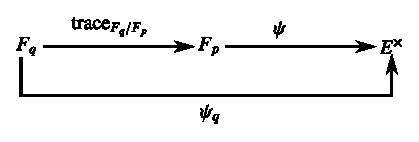
\includegraphics{chap6/fig1.eps}
\end{figure}
Given a character of $\mu_{N}$, i.e. a homomorphism
$$
\chi : \mu_{N}(E)\to E^{\times},
$$
a $p$-adic place $\sfP$ of $E$, with residue field $F_{N(P)}$, and a finite extension $F_{q}$ of this residue field, the map ``reduction mod $\sfP$'' induces an isomorphism
$$
\mu_{N}(E)\xrightarrow{\sim}\mu_{N}(F_{N(P)})=\mu_{N}(F_{q})
$$
Because $F^{\times}_{q}$ is cyclic, we know that $q\equiv 1\mod N$, and that the map $x\to x^{\frac{q-1}{N}}$ defines a surjection
$$
F^{\times}_{q}\twoheadrightarrow \mu_{N}(F_{q})=\mu_{N}(F_{N(P)})\xrightarrow{\sim}\mu_{N}(E)
$$
We define the character $\chi_{q}$ of $F^{\times}_{q}$ as the composite
\begin{figure}[H]
\centering
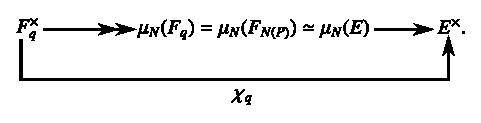
\includegraphics{chap6/fig2.eps}
\end{figure}
The Gauss sum $g_{q}(\psi,\chi,\sfP)$ attached to this situation is defined by the formual
$$
g_{q}(\psi,\chi,\sfP)=\sum\limits_{x\in F^{\times}_{q}}\psi_{q}(x)\chi_{q}(x)
$$
An\pageoriginale elementary computation shows that
$$
g_{q}(\psi,\chi,\sfP)=
\begin{cases}
q-1 & \text{if $\psi$, $\chi$ both trivial}\\
0   & \text{if $\psi$ trivial, $\chi$ non-trivial}\\
-1  & \text{if $\psi$ non-trivial, $\chi$ trivial}
\end{cases}
$$
while
$$
|g_{q}(\psi,\chi,\sfP)|=\sqrt{q}\text{~~ if~~ } \psi,\chi\text{~ both non-trivial}
$$
for any archimedean absolute value on $E$ (cf \cite{art6-key47}).

Now consider the Artin-Schreier curve $X/F_{q}$, defined to be the complete non-singular model of the affine smooth geometrically connected curve over $F_{q}$ with equation
$$
T^{P}-T=X^{N}.
$$
Set theoretically, $X$ consists of this affine curve plus a single rational point at $\infty$. The group $F_{q}\times \mu_{N}(F_{q})$ operates on $X/F_{q}$ curve by the affine formulas
$$
(a,\zeta):(T,X)\to (T+a,\zeta X),
$$
fixing the point at $\infty$. Via the ``reduction mod $\sfP$'' isomorphism
$$
\mu_{N}(E)\xrightarrow{\sim}\mu_{N}(F_{N(\sfP)})=\mu_{N}(F_{q}),
$$
we may view $(\psi,\chi)$ as a character of the group $F_{p}\times \mu_{N}(F_{q})$:
$$
(\psi,\chi)(a,\zeta)=\psi(a)\chi(\zeta).
$$
Thus we may speak of the sums
$$
S(X/F_{q},(\psi,\chi),n)=\frac{1}{pN}\sum\limits_{(a,\zeta)\in F_{p}\times \mu_{N}}\psi(a)\chi(\zeta)\sharp \text{~Fix~} (F^{n}\cdot (a,\zeta)^{-1})
$$
attached to this situation.

\medskip
\noindent
{\bf Lemma \thnum{2.1}.\label{art6-lem2.1}}~{\em If $\chi$ is non-trivial and $\psi$ is arbitrary, then we have}
\begin{equation*}
S(X/F_{q},(\psi,\chi),n)=g_{q^{n}}(\psi,\chi,\sfP).\tag{2.1.1}\label{art6-eq2.1.1}
\end{equation*}

\begin{proof}
It\pageoriginale suffices to treat the case $n=1$, for we have
$$
S(X/F_{q^{n}},(\psi,\chi),1)=S(X/F_{q},(\psi,\chi),n).
$$
We can rewrite $S(X/F_{q},(\psi,\chi),1)$ as
$$
\sum\limits_{x\in X(\overline{F}q)}\frac{1}{pN}\sum\limits_{\substack{(a,\zeta)s.t.\\ F(x)=(a,\zeta)(x)}}\psi(a)\chi(\zeta)
$$
Given any point $x\in X(\overline{F}_{q})$, the set of $(a,\zeta)\in F_{p}\times \mu_{N}$ which satisfy $F(x)=(a,\zeta)(x)$ is either empty or principal homogeneous under the inertia {\em subgroup} $I_{x}$ of $F_{p}\times \mu_{N}$ which {\em fixes} $x$; therefore if the restriction of $(\psi,\chi)$ to this subgroup is {\em non-trivial}, the inner sum above {\em vanishes}. Because $\chi$ is assumed {\em non-trivial}, this vanishing applies to the point at $\infty$ (for which $I_{x}$ is all of $F_{p}\times \mu_{N}$) and to any finite point $(T,0)$ whose $X$-coordinate is zero (then $I_{(T,0)}=\{0\}\times \mu_{N}$).

Given a point $(T,X)$ with $X\neq 0$, we have
$$
F(T,X)=(T^{q},X^{q})
$$
and the inertia subgroup $I_{(T,X)}$ is trival. If there is an element $(a,\zeta)\in F_{p}\times \mu_{N}$ satisfying $F(T,X)=(T+a,\zeta X)$, then it is given by the formulas
$$
a=T^{q}-T, \ \zeta=X^{q-1}
$$
Since the point $(T,X)$ is subject to the defining equation
$$
T^{p}-T=X^{N}
$$
we see that
\begin{align*}
& (X^{N})^{q-1}=(X^{q-1})^{N}=\zeta^{N}=1,\text{~ hence~ } X^{N}\in F^{\times}_{q}, \ \zeta=(X^{N})^{\frac{q-1}{N}}\\[3pt]
& T^{p}-T=X^{N}\in F^{\times}_{q},\\[3pt]
& a=T^{q}-T=\text{~trace}_{F_{q}/F_{p}}(T^{p}-T)=\text{trace}_{F_{q}/F_{p}}(X^{N}).
\end{align*}
For each $u\in F^{\times}_{q}$, the equations $(T^{P}-T=u,X^{N}=u)$ have $pN$ solutions $(T,X)$ over $\overline{F}_{q}$, all of which satisfy
$$
F(T,X)=(a,\zeta)(T,X)
$$
with\pageoriginale the {\em same} $(a,\zeta)$, namely (trace$_{F_{q}/F_{p}}(u)$, $u^{\frac{q-1}{N}}$), and {\em every} point $(T,X)$ which contributes to our sum lies over some $u\in F^{\times}_{q}$. Thus our sum becomes
$$
\sum\limits_{u\in F^{\times}_{q}}\psi(\text{trace}_{F_{q}/F_{p}}(u))\chi(u^{\frac{q-1}{N}})^{\text{dfn}}g_{q}(\psi,\chi,\sfP).
$$
\end{proof}

\medskip
\noindent
{\bf Corollary \thnum{2.2}.\label{art6-coro2.2}}~{\em Let $H^{i}$ denote any of the cohomology groups $H^{i}_{l}(X)\otimes E_{\lambda}$ with $l\neq p$, or $\foprod{H^{i}_{\text{cris}}(X)}{E_{P}}{W}$ of the Artin Schreier curve $X/F_{q}$.}
\begin{itemize}
\item[(1)] {\em If $\psi$ and $\chi$ are both non-trivial, then the eigenspace $(H^{1})^{\psi\cdot \chi}$ is one-dimensional, and we have a direct sum decomposition}
$$
H^{i}=\oplus (H^{1})^{\psi\cdot \chi}
$$
{\em indexed by the ($p-1(N-1)$ pairs $(\psi,\chi)$) of non-trivial characters.}

\item[(2)] {\em The eigenvalue of $F$ on $(H^{1})^{\psi\cdot \chi}$ is $-g_{q}(\psi,\chi,\sfP)$, and for each $n\geq 1$ we have the Hasse-Davenport formula}
$$
-g_{q^{n}}(\psi,\chi,\sfP)=(-g_{q}(\psi,\chi,\sfP))^{n}.
$$

\item[(3)] {\em The group $F_{q}\times \mu_{N}$ acts trivially on both $H^{0}$ and $H^{2}$.}
\end{itemize}

\begin{proof}
That the group acts trivially on both $H^{0}$ and $H^{2}$ follows from the fact that these are one-dimensional spaces on which $F$ always acts as $1$ and $q$ respectively. The descent argument shows that for any automorphism of {\em finite order} $g$ which commutes with $F$, $Fg$ also acts as $1$ and $q$ on $H^{0}$ and $H^{2}$ respectively, and hence that $g$ itself acts trivially on $H^{0}$ and $H^{2}$.

That the multiplicity of $(\psi,\chi)$ in $H^{1}$ is {\em one} when both $\psi$ and $\chi$ are non-trivial follows from the lemma of the previous section, given the identity \eqref{art6-eq2.1.1} and the known absolute value of gauss sums; and assertion (2) above is just a repetition of part of that lemma in this particular case. To see that no other characters occurs in $H^{1}$, we recall that the dimension of $H^{1}$ is known to be $2g$, $g=$ genus of $X$, and so it suffices to verify that $2g=(p-1)(N-1)$. This formula, whose elementary verification we leave to the reader, is in fact valid in any characteristic prime to $N(p-1)$. (Hing: view $T^{P}-T=X^{N}$ an an $N$-fold covering of the $T$-line!)
\end{proof}

We\pageoriginale now turn to the consideration of Jacobi sums. We fix an integer $N\geq 2$ prime to $p$, and a number field $E$ containing the $N$'th roots of unity. Given a $p$-adic place $\sfP$ of $E$, a character $\chi$ of $\mu_{N}$
$$
\chi :\mu_{N}(E)\to E^{\times}
$$
and a finite extension $F_{q}$ of the residue field $F_{N(\sfP)}$ at $\sfP$, we obtain the character $\chi_{q}$
$$
\chi_{q}:F^{\times}_{q}\to E^{\times}
$$
in the manner explained above. Given two characters $\chi$, $\chi'$ of $\mu_{N}$, the Jacobi sum $J_{q}(\chi,\chi',\sfP)$ is defined by the formula
$$
J_{q}(\chi,\chi',\sfP) {\displaystyle{\mathop{=}\limits^{\text{dfn}}}}\sum\limits_{\substack{x\in Fq\\ x\neq 0,1}}\chi_{q}(x)\chi'_{q}(1-x).
$$
An elementary computation (cf \cite{art6-key14}) shows that if the {\em product} $\chi\chi'$ is non-trivial, then for any non-trivial additive character $\psi$ of $F_{p}$, we have the formula
$$
g_{q}(\psi,\chi,\sfP)g_{q}(\psi,\chi',\sfP)=J_{q}(\chi,\chi',\sfP)g_{q}(\psi,\chi\chi',\sfP)
$$
In particular, from the known absolute values of Gauss sums we obtain
$$
|J_{q}(\chi,\chi',\sfp)|=\sqrt{q}
$$
for all archimedean absolute values of $E$, provided that $\chi$, $\chi'$, and $\chi\chi'$ are {\em all} non-trivial.

Now consider the Fermat curve $Y/F_{q}$, defined by the homogeneous equation
$$
X^{N}+Y^{N}=Z^{N}
$$
The group $\mu_{N}\times \mu_{N}$ operates on this curve by the formula
$$
(\zeta_{1},\zeta_{2}):(X,Y,Z)\to (\zeta_{1}X,\zeta_{2}Y,Z).
$$
Viewing $(\chi,\chi')$ as a character of this group
$$
(\chi,\chi')(\zeta_{1},\zeta_{2}) {\displaystyle{\mathop{=}\limits^{\text{dfn}}}}\chi(\zeta_{1})\chi'(\zeta_{2}),
$$
we may speak of the sums $S(Y/F_{q},(\chi,\chi')n)$ attached to this situation.

In\pageoriginale complete analogy with the situation for the Artin-Schreier curve, we have the following lemma and corollary, whose analogous proofs are left to the reader.

\medskip
\noindent
{\bf Lemma \thnum{2.3}.\label{art6-lem2.3}}~{\em If $\chi$ and $\chi'$ are non-trivial characters of $\mu_{N}$ such that $\chi\chi'$ is also non-trivial, then we have, for all $n\geq 1$,}
\begin{equation*}
S(Y/F_{q},(\chi,\chi'),n)=J_{q^{n}}(\chi,\chi',\sfp).\tag{2.3.1}\label{art6-eq2.3.1}
\end{equation*}
\smallskip

\noindent
{\bf Corollary \thnum{2.4}.\label{art6-coro2.4}}~{\em Let $H^{i}$ denote any of the cohomology groups $H^{i}_{l}(Y)\otimes E_{\lambda}$ with $l\neq p$, or $\foprod{H^{i}_{\text{cris}}(X)}{E_{\sfp}}{W}$ of the Fermat curve $Y/F_{q}$.}
\begin{itemize}
\item[(1)] {\em If $\chi$, $\chi'$ and $\chi\chi'$ are all non-trivial, then the eigenspace $(H^{1})^{(\chi,\chi')}$ is one-dimensional, and we have a direct sum decomposition}
$$
H^{1}=\oplus (H^{1})^{(\chi,\chi')}
$$
{\em indexed by the $(N-1)(N-2)$ pairs $(\chi,\chi')$ of non-trivial characters of $\mu_{N}$ whose product $\chi\chi'$ is also non-trivial}.

\item[(2)] {\em The eigenvalue of $F$ on $(H^{1})^{(\chi,\chi')}$ is $-J_{q}(\chi,\chi',\sfP)$, and for each integer $n\geq 1$ we have the Hasse-Davenport formula}
$$
-J_{q^{n}}(\chi,\chi',\sfP)=(-J_{q}(\chi,\chi',\sfP))^{n}.
$$

\item[(3)] {\em The group $\mu_{N}\times \mu_{N}$ operates trivially on both $H^{0}$ and $H^{2}$.}
\end{itemize}

\bigskip
\noindent
{\bf III. The problem of ``explicitly'' computing Frobenius.} We return now to the general setting of a projective, smooth, and geometrically connected variety $X/F_{q}$ of dimension $d$. A tantalizing feature of all the cohomology theories that we have been discussing is that when the variety $X$ ``lifts'' to characteristic zero, then the corresponding cohomology groups $H^{i}(X)$ have an ``elementary'' description in terms of standard algebro-geometric and topological invariants of the lifting.

More precisely, suppose we are given a projective smooth scheme $X$ over $W(F_{q})$, together with an $F_{q}$-isomorphism of its special fibre with $X$. (This is a rather strong notion of what a ``lifting'' of $X$ should mean, but it is adequate for our purposes, and it avoids certain technical problems related to ramification). Then there is a canonical isomorphism
$$
H^{i}_{\text{cris}}\to H^{i}_{\DR}(X/W(F_{q}))
$$
of\pageoriginale $H^{i}_{\text{cris}}$ with the algebraic de Rham cohomology of the lifting (cf \cite{art6-key19}, \cite{art6-key27}).

To discuss $H^{i}_{l}(X)$, we must in addition choose (!) a complex embedding
$$
W(F_{q})\hookrightarrow C.
$$
By means of such an embedding, we may ``extend scalars'' to obtain from $X/W$ a projective smooth complex variety $X_{C}$, and an associated complex manifold $X^{\text{an}}_{C}$. For each prime number $l\neq p$, there is a canonical isomorphism
$$
H^{i}_{l}(X)\to \fprod{H^{i}_{\text{top}}(X^{\text{an}}_{C},Z)}{Z_{l}}{Z},
$$
where $H^{i}_{\text{top}}$ denotes the usual ``topological'' cohomology.

To emphasize the similarity between these two sorts of isomorphisms, recall that by GAGA and the holomorphic Poincar\'e lemma, we have a canonical isomorphism
\[
\xymatrix{
\foprod{H^{i}_{\DR}(X/W)}{C}{W}\ar[r]^{\sim} & H^{i}_{\DR}(X/C)\ar[r]^{\sim} & H^{i}_{\top}(X^{an}_{C},C)\\
                                         &                           & \foprod{H^{i}_{\top}(X^{an},Z)}{C}{Z}\ar[u]^{\rotatebox{90}{$\backsim$}}
}
\]

Unfortunately, these rather concrete descriptions of the various cohomology {\em groups} $H^{i}(X)$ shed little light on their {\em functoriality}. In the rather unusual case of an $F_{q}$-endomorphism $f:X\to X$ which happens to admit a lifting to a $W$-endomorphism
$$
f:X\to X,
$$
we have the simple formulas
$$
\begin{cases}
f^{*}\text{~ on~ } H^{i}_{\text{cris}}(X)=f^{*}\text{~ on~ } H^{i}_{\DR}(X/W)\\
f^{*}\text{~ on~ } H^{i}_{l}(X)=(f^{an}_{C})^{*}\otimes 1\text{~ on~ } \foprod{H^{i}_{\top}(X^{an}_{C},Z)}{Z_{l},l\neq p}{Z}
\end{cases}
$$
But for those $f$ which do not lift, we are left somewhat in the dark as to an explicit description of the map $f^{*}$ on cohomology.

Suppose for example that a finite group $G$ operates on $X$ by $F_{q}$-automorphisms, and that this action can be lifted to an action of $G$ on $X$ by $W$-automorphisms. Then our canonical isomorphisms
$$
\begin{cases}
H^{i}_{\text{cris}}(X)\xrightarrow{\sim} H^{i}_{\DR}(X/W)\\
H^{i}_{l}(X)\xrightarrow{\sim} H^{i}_{\top}(X^{an}_{C},Z)\otimes Z_{l}\text{~ for~ } l\neq p
\end{cases}
$$\pageoriginale
are $G$-equivariant. In particular, we can ``explicitly compute'' the multiplicities of the various complex irreducible representations $\rho$ of $G$ in the cohomology of $X$, and we can ``explicitly compute'' the various isotypical components of the cohomology. If it turns out that a given irreducible representation $\rho$ occurs in a given $H^{i}$ with multiplicity {\em one}, then we know a priori that $F$ must operate on the corresponding isotypical component $(H^{i})^{\rho}$ as a {\em scalar}, and we know this even when $F$ itself does not lift.

For example, we could recover the isotypical decomposition of $H^{1}$ of the Fermat curve $Y$ under the action of $\mu_{N}\times \mu_{N}$ by lifting the curve and the group action (use the ``same'' equations) and making an explicit algebro-geometric or topological calculation of the corresponding isotypical decomposition in characteristic zero. In terms of, say, the crystalline cohomology, we obtain an $F$-stable decomposition
$$
H^{1}_{\text{cris}}(Y)\xrightarrow{\sim}H^{1}_{\DR}(Y/W)^{(\chi,\chi')};
$$
in a basis of $H^{1}_{\DR}(Y/W)$ adapted to this decomposition, the matrix of $F$ is the diagonal matrix
$$
\left(
\begin{matrix}
\ddots & & O\\
       & -J_{q}(\chi,\chi',\sfP) &\\
O & & \ddots
\end{matrix}
\right)
$$

However, it must be borne in mind that the Fermat curve is atypically susceptible to this sort of analysis; it is unusual for a group action, even on a curve, to be liftable to characteristic zero. For example, the action of $F_{p}$ on an Artin-Schreier covering of $A^{1}$ doesn't lift to characteristic zero. To get around this non-liftability, we will be led to consider the Washnitzer-Monsky cohomology as well, in Chapter VII.

\bigskip
\noindent
{\bf IV. {\boldmath$H^{1}$} and abelian varieties; preliminaries.} Consider an abelian variety $A/F_{q}$, say of dimension $g$. We denote by $\End(A)$ the ring of all $F_{q}$-endomorphisms of $A$, and by $\End(A)^{0}$ the opposite ring. As $Z$-modules, they are free and finitely generated. For each prime $l\neq p$, the\pageoriginale cohomology group $H^{1}_{l}(A)$ is a free $Z_{l}$-module of rank $2g$, and is an $\End (A)^{0}$-module. (It is also the case that $H^{1}_{\text{cris}}(A)$ is a free $W$-module of rank $2g$, and is an $\End(A)^{0}$-module, but we will not make use of this fact for the moment).

\medskip
\noindent
{\bf Lemma \thnum{4.1}.\label{art6-lem4.1}}~{\em If $E$ is a number field, and $\lambda$ is a place of $E$ lying over a prime $l\neq p$, the natural maps}
\[
\xymatrix{
\foprod{\End(A)^{0}}{E}{Z}\ar[r] & \foprod{\End(A)^{0}}{E_{\lambda}}{Z}\ar[r] & \foprod{\End_{Z_{l}}(H^{1}_{l}(A))}{E_{\lambda}}{Z_{l}}\\
                                &                                         & \End_{E_{\lambda}}(\foprod{H^{1}_{l}(A)}{E_{\lambda}}{Z_{l}})\ar[u]^-{\rotatebox{90}{$\backsim$}}
}
\]
{\em are all injective.}

\begin{proof}
The first map is injective simply because $E\subset E_{\lambda}$, and because $\End(A)^{0}$ is flat over $Z$. The second map is obtained from the map
$$
\foprod{\End(A)^{0}}{Z_{l}}{Z}\to \End_{Z_{l}}(H^{1}_{l}(A))
$$
by tensoring over $Z_{l}$ with the flat $Z_{l}$-module $E_{\lambda}$. In fact this flatness is irrelevant, for the above map is injective and has $Z_{l}$-flat cokernel. To see this, recall that (by the Kummer sequence in etale cohomology) we have a canonical isomorphism
$$
H^{1}_{l}(A)\simeq T_{l}(\Pic^{0}(A))(-1)\simeq \Hom(T_{l}(A),Z_{l}),
$$
under which the map considered above is the ``opposite'' of the map
$$
\foprod{\End(A)}{Z_{l}}{Z}\to \End_{Z_{l}}(T_{l}(A))
$$
Our assertion of its injectivity with $Z_{l}$-flat cokernel is equivalent to the injectivity of (any one of) the maps
$$
\End(A)/l^{n}\End(A)\to \End(A_{l^{n}}),
$$
and this injectivity follows from the exactness of the sequence
$$
0\to A_{l^{n}}\to A \xrightarrow{l^{n}} A\to 0
$$
in the etale topology.
\end{proof}

Now consider a projective, smooth and geometrically connected variety $X/F_{q}$. Its Albanese variety $\Alb(X)$ is an abelian variety over $F_{q}$ which\pageoriginale for our purposes is best viewed as the {\em dual} of the Picard variety $\Pic(X)$, itself defined in terms of the Picard scheme $\Pic_{X/F_{q}}$ as $(\Pic^{0}_{X/F_{q}})^{\red}$. The Kummer sequence in etale cohomology together with the duality of abelian varieties gives isomorphisms for each $l\neq p$
\begin{align*}
& H^{1}_{l}(X)\xrightarrow{\sim}T_{l}(\Pic(X))(-1)\tag{4.1.1}\label{art6-eq4.1.1}\\
& H^{1}(\Alb(X))\xrightarrow{\sim}T_{l}(\Pic(\Alb(X))(-1)=T_{l}(\Pic(X))(-1)\tag{4.1.2}\label{art6-eq4.1.2}
\end{align*}
which combine to give a canonical isomorphism
\begin{equation*}
H^{1}_{l}(X)\simeq H^{1}_{l}(\Alb(X))\quad\text{for}\quad l\neq p\tag{4.1.3}\label{art6-eq4.1.3}
\end{equation*}

Suppose now that a finite group $G$ operates on $X$ by $F_{q}$-automor\-phisms. Let $\rho$ be an absolutely irreducible representation of $G$ defined over a number field $E$, which occurs in $H^{1}(X)$ with multiplicity $r$. Denote by
$$
P_{1,\rho}(T)=1+a_{1}(\rho)T+\cdots+a_{r}(\rho)T^{r}\in \mathscr{O}_{E}[T]
$$
the reversed characteristic polynomial of $F$ acting on the space 
$$
\Hom_{G}(\rho,H^{1}(X))
$$ 
of occurrences of $\rho$ in $H^{1}$;
$$
P_{1,\rho}(T)=\det (1-TF|\Hom_{G}(\rho,H^{1}(X)).
$$

Let us denote by $\Proj(\rho)\in \mathscr{O}_{E}[1/\sharp G][G]$ the projector
$$
\Proj (\rho)=\dfrac{\deg (\rho)}{\sharp G}\sum\limits_{g\in G}\tr(\rho(q^{-1}))\cdot [g].
$$
By functoriality, $G$ also operates on $\Alb(X)$ by $F_{q}$-automorphisms, so we may view $\Proj(\rho)$, or indeed any element of the $\mathscr{O}_{E}[1/\sharp G]$-group ring of $G$, as defining an element of $\End(\Alb(X))\otimes \mathscr{O}_{E}[1/\sharp G]$.

\medskip
\noindent
{\bf Proposition \thnum{4.2}.\label{art6-prop4.2}}~{\em In the above situation, we have the formula}
\begin{align*}
& (F^{r}+a_{1}(\rho)F^{r-1}+\cdots+a_{r}(\rho))\cdot \Proj (\rho)=0\\
& \Proj (\rho)\cdot (F^{r}+a_{1}(\rho)F^{r-1}+\cdots+a_{r}(\rho))=0
\end{align*}
{\em in $\End(\Alb(X))\otimes \mathscr{O}_{E}[1/\sharp G]$. (N.B. since $F$ and $G$ commute, these formulas are equivalent).}

\begin{proof}
Since $\End(\Alb(X))\otimes \mathscr{O}_{E}[1/\sharp G]$ is contained in $\End(\Alb(X))\otimes E$, which is in turn contained in $\End(\foprod{H^{1}_{l}(\Alb(X))}{E_{\lambda}}{Z})$ for\pageoriginale any $l\neq p$, it suffices to verify that $F^{r}+a_{1}(\rho)F^{r-1}+\cdots+a_{r}(\rho)$ annihilates $(H^{1}(\Alb(X))^{\rho}$. But this space is isomorphic to $(H^{1}(X))^{\rho}$, which is in turn isomorphic to $\rho\otimes \Hom_{G}(\rho,H^{1}(X))$, with $F$ acting through the second factor, so we need the above polynomial in $F$ to annihilate $\Hom_{G}(\rho,H^{1}(X))$. This follows from the Cayley-Hamilton theorem.
\end{proof}

\medskip
\noindent
{\bf Corollary \thnum{4.3}.\label{art6-coro4.3}}~{\em Let $D$ be any contravariant additive functor from the category of abelian varieties over $F_{q}$ to the category of $\mathscr{O}_{E}[1/\sharp G]$-modules.}

{\em For any element $m\in (D(\Alb(X)))^{\rho}$, we have}
$$
F^{r}(m)+a_{1}(\rho)F^{r-1}(m)+\cdots+a_{r}(\rho)\cdot m=0
$$
{\em in $D(\Alb(X))$.}
\smallskip

We will apply this to the functor ``Dieudonne module of the formal group of $A$,'' constructed a la Honda.

\bigskip
\noindent
{\bf V. Explicit Dieudonn\'e Theory \`a la Honda; generalities}
\smallskip

\noindent
{\bf \thnum{5.1}.\label{art6-sec5.1} Basic Constructions.}
We being by recalling the notions of formal Lie variety and formal Lie groups. Over any ring $R$, an $n$-dimensional formal Lie variety $V$ is a set-valued functor on the category of adic $R$-algebras which is isomorphic to the functor.
$$
R'\to n\text{-tuples of topologically nilpotent elements of $R'$.}
$$
A system of coordinates $X_{1},\ldots,X_{n}$ for $V$ is the choice of such an isomorphism. The coordinate ring $A(V)$ is the $R$-algebra of all maps of set-functors from $V$ to the ``identical functor'' $R'\mapsto R'$; in coordinates, $A(V)$ is just the power series ring $R[[X_{1},\ldots,X_{n}]]$. Although the ideal $(X_{1},\ldots,X_{n})$ in $A(V)$ is {\em not} intrinsic, the adic topology it defines on $A(V)$ is intrinsic, and $A(V)$, viewed as an adic $R$-algebra, represents the functor $V$.

The de Rham cohomology groups $H^{i}_{\DR}(V/R)$ are the $R$-modules obtained by taking the cohomology groups of the formal de Rham complex $\Omega^{\bigdot}_{V/R}$ (the separated completion of the ``literal'' de Rham complex of $A(V)$ as $R$-algebra); in terms of coordinates $X_{1},\ldots,X_{n}$ for $V$, $\Omega^{\bigdot}_{V/R}$ is the exterior algebra over $A(V)$ on $dX_{1},\ldots,dX_{n}$, with exterior differentiation $d:\Omega^{i}\to \Omega^{i+1}$ given by the customary formulas.

A\pageoriginale pointed formal Lie variety $(V,0)$ over $R$ is a formal Lie variety $V$ over $R$ together with a marked point ``0'' $\epsilon V(R)$. A formal Lie group $G$ over $R$ is a ``group-object'' in the category of formal Lie varieties over $R$.

We denote by $CFG(R)$ the additive category of commutative formal Lie groups over $R$. The ``sum'' map
$$
\text{sum : }G\times G\to G
$$
as well as the two projections
$$
\pr_{1},\pr_{2} : G\times G\to G
$$
are morphisms in this category. For $G\in CFG(R)$, we define $D(G/R)$ to be the $R$-submodule of $H^{1}_{\DR}(G/R)$ consisting of the primitive elements, i.e. the elements $a\in H^{1}_{\DR}(G/R)$ such that
$$
\text{sum}^{*}(a)=\pr^{*}_{1}(a)+\pr^{*}_{2}(a)\text{~~ in~~ } H^{1}_{\DR}((G\times G)/R).
$$

\medskip
\noindent
{\bf Lemma \thnum{5.1.1}.\label{art6-lem5.1.1}}~{\em Over any ring $R$, the construction $G\to D(G/R)$ defines a (contravariant) additive functor from $CFG(R)$ to $R$-modules.}
\smallskip

\begin{proof}
This is a completely ``categorical'' result. To begin, let $G$, $G'\in CFG(R)$, and let $f:G'\to G$ be a homomorphism. Then the diagram
\[
\xymatrix{
G'\times G'\ar[r]^-{\text{sum}}\ar[d]^-{f\times f} & G'\ar[d]^-{f}\\
G\times G\ar[r]^-{\text{sum}} & G
}
\]
commutes, as do the analogous diagrams with ``sum'' replaced by $\pr_{1}$ or $\pr_{2}$. Therefore given any element $a\in H^{1}_{\DR}(G/R)$, we have
\begin{align*}
\text{sum}^{*}(f^{*}(a))-\pr^{*}_{1}(f^{*}(a))-\pr_{2}(f^{*}(a))=\\
(f\times f)^{*}(\text{sum}^{*}(a)-\pr^{*}_{1}(a)-\pr^{*}_{2}(a)).
\end{align*}
In particular, if $a\in D(G/R)$ then $f^{*}(a)\in D(G'/R)$.

Given $f_{1}$, $f_{2}$ homomorphisms $G'\to G$, let $f_{3}$ be their sum. Then we have a commutative diagram
\begin{figure}[H]
\centering
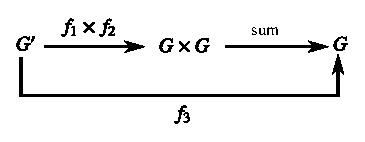
\includegraphics{chap6/fig3.eps}
\end{figure}\pageoriginale
as well as a commutative diagram
\begin{figure}[H]
\centering
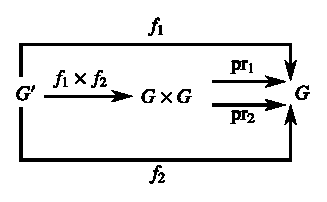
\includegraphics{chap6/fig4.eps}
\end{figure}
Therefore for any $a\in H^{1}_{\DR}(G/R)$, we have
$$
f^{*}_{3}(a)-f^{*}_{1}(a)-f^{*}_{2}(a)=(f_{1}\times f_{2})^{*}(\text{sum}^{*}(a)-\pr_{1}^{*}(a)-\pr_{2}^{*}(a)).
$$
In particular, if $a\in D(G/R)$, then $f^{*}_{3}(a)=f^{*}_{1}(a)+f^{*}_{2}(a)$.
\end{proof}

For the remainder of this section, we will consider a ring $R$ which is flat over $Z$, and an ideal $I\subset R$ which has divided powers. The flatness means that if we denote by $K$ the $Q$-algebra $R\otimes Q$, then $R\subset K$. That the ideal $I\subset R$ has divided powers means that for any integer $n\geq 1$, and any element $i\in I$, the element $i^{n}/n!$ of $K$ actually lies in $I$.

Given a formal Lie variety $V$ over $R$, we denote by $V\otimes K$ the formal Lie variety over $K$ obtained by extension of scalars. In terms of coordinates $X_{1},\ldots,X_{n}$ for $V$, $A(V\otimes K)$ is the power-series ring $K[[X_{1},\ldots,X_{n}]]$. We say that an element of $A(V\otimes K)$ is {\em integral} if it lies in the subring $A(V)$; similarly, an element of the de Rham complex $\Omega_{V\otimes K/K}$ is said to be {\em integral} if it lies in the subcomplex $\Omega_{V/R}$.

\medskip
\noindent
{\bf Lemma \thnum{5.1.2}.\label{art6-lem5.1.2}}~{\em Let $(V,0)$ be a pointed Lie variety over a $Z$-flat ring $R$. Then exterior differentiation induces an isomorphism of $R$-modules}
$$
\frac{\{f\in A(V\otimes K)|f(0)=0,df\text{ integral}\}}{\{f\in A(V)|f(0)=0\}}\xrightarrow{\sim}H^{1}_{\DR}(V/R)
$$
{\em which is compatible with morphisms of pointed Lie varieties.}

\begin{proof}
Because\pageoriginale $K$ is a $Q$-algebra, the formal Poincare lemma gives $H^{0}_{\DR}(V\otimes K/K)=K$, $H^{i}_{\DR}(V\otimes K/K)=0$ for $i\geq 1$. Therefore any closed one-form on $V/R$ can be written as df with $f\in A(V\otimes K)$, and this $f$ is unique up to a constant. If we normalize $f$ by the condition $f(0)=0$, we get the asserted isomorphism.
\end{proof}

\smallskip
\noindent
{\bf Key Lemma \thnum{5.1.3}.\label{art6-keylem5.1.3}}~{\em Let $(V,0)$ and $(V',0)$ be pointed formal Lie varieties over a $Z$-flat ring $R$, and let $I\subset R$ be an ideal with divided powers. If $f_{1}$, $f_{2}$ are two pointed morphisms $V'\to V$ such that $f_{1}=f_{2}$ mod $I$, then the induced maps}
$$
f^{*}_{1}, f^{*}_{2} : H^{1}_{\DR}(V/R)\to H^{1}_{\DR}(V'/R)
$$
{\em are equal.}
\smallskip

\begin{proof}
Let $\varphi_{1}$, $\varphi_{2}$ denote the algebra homomorphisms $A(V)\to A(V')$ corresponding to $f_{1}$ and $f_{2}$. By the previous lemma, we must show that for every element $f\in A(V\otimes K)$ with $f(0)=0$ and $df$ integral, the difference $\varphi_{1}(f)-\varphi_{2}(f)$ lies in $A(V')$, i.e. is itself integral. (Because $f_{1}$ and $f_{2}$ were assumed pointed, this difference automatically has constant term zero).

In terms of pointed coordinates $X_{1},\ldots,X_{n}$ for $V'$ and $Y_{1},\ldots,Y_{m}$ for $V$, the maps $\varphi_{1}$ and $\varphi_{2}$ are given by substitutions
\begin{align*}
\varphi_{1}(f(Y)) &=f(\varphi_{1}(X))\\
\varphi_{2}(f(Y)) &= f(\varphi_{2}(X))
\end{align*}
where $\varphi_{1}(X)$, $\varphi_{2}(X)$ are $m$-tuples of series in $X=(X_{1},\ldots,X_{n})$ without constant term. The hypothesis $f_{1}=f_{2}$ mod $I$ means that the component-by-component difference $\Delta=\varphi_{2}(X)-\varphi_{1}(X)$ satisfies 
$$
\Delta(0)=0, \Delta\text{~ has all coefficients in $I$}.
$$
We now compute using Taylor's formula, and usual multi-index notations:
\begin{align*}
\varphi_{2}(f) -\varphi_{1}(f) &= f(\varphi_{2}(X))-f(\varphi_{1}(X))\\
&= f(\varphi_{1}(X)+\Delta)-f(\varphi_{1}(X))\\
&=\sum\limits_{|\underline{n}|\geq 1}\frac{\Delta^{\underline{n}}}{(\underline{n})!}\left(\frac{\partial^{\underline{n}}}{\partial Y^{\underline{n}}}f\right)(\varphi_{1}(X)).
\end{align*}
This\pageoriginale last sum is $X$-adically convergent (because $\Delta$ has no constant term), and its individual terms are integral (because $\Delta$ has coefficients in the divided power ideal $I$, the terms $\Delta^{\underline{n}}/(\underline{n})!$ all have coefficients in $I$, and hence in $R$; because $df$ is integral, all the first partials $\partial f/\partial Y_{i}$ are integral, and a fortiori all the higher partials are integral).
\end{proof}

\medskip
\noindent
{\bf Theorem \thnum{5.1.4}.\label{art6-thm5.1.4}}~{\em Let $R$ be a $Z$-flat ring, and $I\subset R$ a divided power ideal. Let $G$, $G'$ be commutative formal Lie groups over $R$, and denote by $G_{0}$, $G'_{0}$ the commutative formal Lie groups over $R_{0}=R/I$ obtained by reduction mod $I$.}
\begin{itemize}
\item[(1)] {\em If $f:G'\to G$ is any morphism of pointed formal Lie varieties whose reduction mod $I$, $f_{0}:G'_{0}\to G_{0}$, is a group homomorphism, then the induced map $f^{*}:H^{1}_{\DR}(G/R)\to H^{1}_{\DR}(G'/R)$ maps $D(G/R)$ to $D(G'/R)$.}

\item[(2)] {\em If $f_{1}$, $f_{2}$, $f_{3}$ are three maps $G'\to G$ of pointed formal Lie varieties whose reductions mod $I$ are group homomorphisms which satisfy $(f_{3})_{0}=(f_{1})_{0}+(f_{2})_{0}$ in $\Hom(G'_{0},G_{0})$, then for any element $a\in D(G/R)$ we have}
$$
f^{*}_{1}(a)+f^{*}_{2}(a)=f^{*}_{3}(a).
$$
\end{itemize}

\begin{proof}
If $f:G'\to G$ is a pointed map which reduces mod $I$ to a group homomorphism, the diagram
\[
\xymatrix{
G'\times G'\ar[d]^-{f\times f}\ar[r]^-{\text{sum}} & G'\ar[d]^-{f}\\
G\times G\ar[r]^-{\text{sum}} & G
}
\]
commutes mod $I$, i.e.
$$
\text{sum~} (f\times f)\equiv f\text{~sum}\quad \mod I.
$$
and hence for any $a\in H^{1}_{\DR}(G/R)$ we have, by the previous lemma,
$$
(f\times f)^{*}(\text{sum}^{*}(a))=\text{sum}^{*}(f^{*}(a))
$$
The analogous diagrams with ``sum'' replaced by $\pr_{1}$ or $\pr_{2}$ commute, hence
$$
(f\times f)^{*}(\pr_{i}^{*}(a))=\pr^{*}_{i}(f^{*}(a))\quad\text{for~ } i=1,2.
$$\pageoriginale
Combining these, we find
\begin{align*}
& (f\times f)^{*}(\text{sum}^{*}(a)-\pr^{*}_{1}(a)-\pr^{*}_{2}(a))=\\
& \text{sum}^{*}(f^{*}(a))-\pr^{*}_{1}(f^{*}(a))-\pr^{*}_{2}(f^{*}(a)).
\end{align*}
In particular, if $a\in D(G/R)$ then $f^{*}(a)\in D(G'/R)$.

Similarly, if $f_{1}$, $f_{2}$ and $f_{3}$ are as in the assertion of the theorem, the diagram
\begin{figure}[H]
\centering
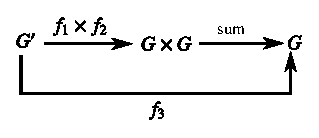
\includegraphics{chap6/fig5.eps}
\end{figure}
commutes mod $I$, and the diagram
\begin{figure}[H]
\centering
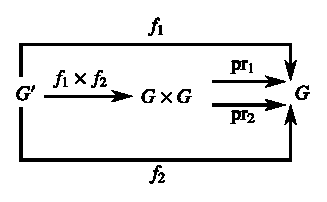
\includegraphics{chap6/fig4.eps}
\end{figure}
commutes. So again using the preceding lemma, we see that for any $a\in H^{1}_{\DR}(G/R)$, we have
$$
f^{*}_{3}(a)-f^{*}_{1}(a)-f^{*}_{2}(a)=(f_{1}\times f_{2})^{*}(\text{Sum}^{*}a)-\pr^{*}_{1}(a)-\pr^{*}_{2}(a)).
$$
In particular, for $a\in D(G/R)$, we obtain the asserted formula
$$
f^{*}_{3}(a)=f^{*}_{1}(a)+f^{*}_{2}(a).
$$
\end{proof}

Let $CFG(R;R_{0})$ denote the additive category whose {\em objects} are the commutative formal Lie groups over $R$, but in which the morphisms are the homomorphisms between their reductions mod $I$:
$$
\Hom_{CFG(R,R_{0})}(G',G)=\Hom(G'_{0},G_{0}).
$$
Given a homomorphism $f_{0}:G'_{0}\to G_{0}$, it always lifts to a pointed morphism\pageoriginale $f:G'\to G$ of formal Lie varieties (just lift its power-series coefficients one-by-one, and keep the constant terms zero).

According to the theorem, the induced map
$$
f^{*}:D(G/R)\to D(G'/R)
$$
is {\em independent} of the choice of pointed lifting $f$ of $f_{0}$. So it makes sense to denote the induced map
$$
(f_{0})^{*}:D(G/R)\to D(G'/R).
$$

\medskip
\noindent
{\bf Theorem \thnum{5.1.5}.\label{art6-thm5.1.5}}~{\em Let $R$ be a $Z$-flat ring, and $I\subset R$ a divided power ideal. Then the construction $G\mapsto D(G/R)$, $f_{0}\mapsto (f_{0})^{*}=$ (any pointed lifting)$^{*}$ defines a contravariant additive functor from the category $CFG(R;R_{0})$ to the category of $R$-modules.}
\smallskip

\begin{proof}
This is just a restatement of the previous theorem.
\end{proof}

\begin{remarks*}
\begin{itemize}
\item[(1)] Thanks to Lazard \cite{art6-key33}, we know that every commutative formal Lie group $G_{0}$ over $R_{0}$ lifts to a commutative formal Lie group $G$ over $R$. If $G'$ is another lifting of $G_{0}$, then the identity endomorphism of $G_{0}$ is an isomorphism of $G'$ with $G$ in the category $CFG(R;R_{0})$. Formation of the induced isomorphism $D(G/R)\xrightarrow{\sim}D(G'/R)$ provides a transitive system of identifications between the $D$'s of all possible liftings. In this way, it is possible to view the construction
$$
G_{0}\mapsto D(G/R),\text{~ where $G$ is some lifting of $G_{0}$}
$$
as providing a contravariant additive functor from $CFG(R_{0})$ to the category of $R$-modules. We will not pursue that point of view here.

\item[(2)] Even without appealing to Lazard, one can proceed in an elementary fashion by observing that any commutative formal Lie group $G_{0}$ over $R_{0}$ can certainly be lifted to a formal Lie ``monoid with unit'' $M$ over $R$ (simply lift the individual coefficients of the group law, and always lift $0$ to $0$). For a monoid, one can still define $D(M/R)$ as the primitive elements of $H^{1}_{\DR}(M/R)$, and one can still show exactly as before that the construction
$$
G_{0}\to D(M/R),\quad M\text{~ any monoid lifting of $G_{0}$}
$$
defines\pageoriginale a contravariant additive functor from $CFG(R_{0})$ to $R$-modu\-les.
\end{itemize}
\end{remarks*}

\noindent
{\em A variant.} The reader cannot have failed to notice the purely formal nature of most of our arguments. We might as well have begun with {\em any} contravariant functor $H$ from formal Lie varieties over a $Z$-flat ring $R$ to $R$-modules for which the key lemma (\ref{art6-keylem5.1.3}) holds. One such $H$, which we will denote $H^{1}_{\DR}(V/R;I)$, is defined as $H^{1}$ of the {\em subcomplex} of the de Rham complex of $V/R$
$$
``IA(V)''\to \Omega^{1}_{V/R}\to \Omega^{2}_{V/R}\to \ldots
$$
where ``$IA(V)$'' denotes the kernel of reduction mod $I$:
$$
``IA(V)''=\Ker(A(V)\twoheadrightarrow A(V_{0})).
$$
In terms of coordinates for $V$, ``$IA(V)$'' is the ideal consisting of those series all of whose coefficients lie in $I$. The analogue of lemma (\ref{art6-lem5.1.2}) becomes
$$
\frac{\{f\in A(V\otimes K)|f(0)=0,dt\text{~integral}\}}{\{f\in ``IA(V)''|f(0)=0\}}\xrightarrow{\displaystyle{\mathop{\sim}\limits^{d}}}H^{1}_{\DR}(V/R;I).
$$
This much makes sense for {\em any} ideal $I\subset R$. If $I$ has divided powers, then the proof of the key lemma (\ref{art6-lem5.1.3}) is almost word-for-word the same. (It works because the terms $\Delta^{\underline{n}}/(\underline{n})!$ all have coefficients in $I$.)

The corresponding theory, ``primitive elements in $H^{1}_{\DR}(G/R;I)$,'' is denoted $D_{1}(G/R)$. In terms of coordinates $X=(X_{1},\ldots,X_{n})$ for $G$, we have the explicit description
{\fontsize{10}{12}\selectfont
\begin{multline*}
D_{1}(G/R)=\\
=\frac{\{f\in K[[X]]|f(0)=0,df\text{~integral, } f(X{\displaystyle{\mathop{+}\limits_{G}}Y})-f(X)-f(Y)\in I[[X,Y]]\}}{\{f\in I[[X]]|f(0)=0\}}
\end{multline*}}\relax
as compared with the explicit description
\begin{multline*}
D(G/R)=\\
=\frac{\{f\in K[[X]]|f(0)=0,df\text{~integral, } f(X{\displaystyle{\mathop{+}\limits_{G}}Y})-f(X)-f(Y)\text{~integral}\}}{\{f\in R[[X]]|f(0)=0\}}
\end{multline*}
For\pageoriginale ease of later reference we summarize the above discussion in a theorem.

\medskip
\noindent
{\bf Theorem \thnum{5.1.6}.\label{art6-thm5.1.6}}~{\em Let $R$ be a $Z$-flat ring, and $I\subset R$ a divided power ideal. The key lemma (\ref{art6-lem5.1.3}) holds for $H^{1}_{\DR}(V/R;I)$, and theorems \eqref{art6-thm5.1.4} and \eqref{art6-thm5.1.5} hold for $D_{1}(G/R)$.}
\smallskip

The natural map $D_{1}\to D$ is not an isomorphism, but its kernel and cokernel are visibly killed by $I$. In the work of Honda and Fontaine, it is $D_{1}$ rather than $D$ which occurs; in the work of Grothendieck and Mazur-Messing (\cite{art6-key17}, \cite{art6-key35}), it is $D$ which arises more naturally.

Let us denote by $\underline{\omega}_{G/R}$ the $R$-module of translation-invariant, or what is the same, primitive, one-forms on $G/R$. Because $G$ is commutative, every element $w\in \underline{\omega}_{G/R}$ is a closed form, so we have natural maps
\[
\xymatrix{
\underline{\omega}_{G/R}\ar[r] & D_{1}(G/R)\ar[d]\\
                              & D(G/R)
}
\]
(Notice that in the extreme case $I=(0)$, the map $\underline{\omega}\to D_{1}$ is an isomorphism!)

\medskip
\noindent
{\bf Lemma \thnum{5.1.7}.\label{art6-lem5.1.7}}~{\em Suppose $R$ flat over $Z$, and $I\subset R$ an ideal. We have exact sequences}
\begin{align*}
& 0\to \Hom_{R\text{-groups}}(G,G_{a})\xrightarrow{d}\underline{\omega}_{G/R}\to D(G/R)\\
& 0\to |Hom_{R/I\text{-groups}}(\foprod{G}{(R/I)}{R},(G_{a})_{R/I})\to D_{1}(G/R)\to D(G/R)
\end{align*}

\begin{proof}
The first is the special case $I=0$ of the second; the second is clear from the explicit description of $D_{1}$ and $D$ given above.
\end{proof}

\medskip
\noindent
{\bf Corollary \thnum{5.1.8}.\label{art6-coro5.1.8}}~{\em If $\Hom_{R\text{-groups}}(G,G_{a})=0$, then the natural maps}
$$
\underline{\omega}_{G}\to D_{1}(G/R)\quad\text{and}\quad \underline{\omega}_{G}\to D(G/R)
$$
{\em are injective.}
\smallskip

The reader interested in obtaining the limit formula for Jacobi sums conjectured\pageoriginale by Honda may skip the rest of this chapter! Others may also be tempted.

\setcounter{section}{5}
\setcounter{subsection}{1}
\subsection{Interpretation via Ext a La Mazur-Messing}\label{art6-sec5.2}
We denote by 
$$
\Ext(G,G_{a})
$$ 
the group of isomorphism classes of extensions of $G$ by $G_{a}$, i.e. of short exact sequences
$$
0\to G_{a}\to E\to G\to 0
$$
of abelian f.p.p.f. sheaves on (Schemes/$R$). We denote by $\Ext^{\text{rigid}}(G,G_{a})$ the group of isomorphism classes of ``rigidified extensions,'' i.e. pairs consisting of an extension of $G$ by $G_{a}$ together with a {\em splitting} of the corresponding extension of Lie algebras:
\begin{figure}[H]
\centering
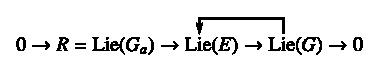
\includegraphics[scale=1.05]{chap6/fig6.eps}
\end{figure}
Because $\Lie(G)$ is a free $R$-module of rank $n=\dim (G)$, any extension of $G$ by $G_{a}$ admits such a rigidification, which is indeterminate up to an element of $\Hom(\Lie(G),\Lie(G_{a}))=\underline{\omega}_{G/R}$. Passing to isomorphism classes and remembering that the set of splittings of a trivial extension of $G$ by $G_{a}$ is itself principal homogeneous under $\Hom(G,G_{a})$, we obtain a four-term exact sequence (valid over {\em any} ring $R$)
$$
\Hom(G,G_{a})\xrightarrow{d}\underline{\omega}_{G}\to \Ext^{\text{rigid}}(G,G_{a})\to \Ext(G,G_{a})\to 0
$$


\smallskip
\noindent
{\bf Theorem \thnum{5.2.1}.\label{art6-thm5.2.1}}~{\em If $R$ is flat over $Z$, there is a natural isomorphism}
$$
D(G/R)\xleftarrow{\sim}\Ext^{\text{rigid}}(G,G_{1})
$$
{\em in terms of which the resulting four term exact sequence}
$$
0\to \Hom(G,G_{a})\to \underline{\omega}_{G}\to D(G/R)\to \Ext(G,G_{a})\to 0
$$
{\em is the concatenation of the three-term sequence of \eqref{art6-keylem5.1.3} and the map} $D(G/R)\to \Ext(G,G_{a})$ defined by
\begin{gather*}
f\to \text{~the class of the symmetric 2-cocycle}\\[3pt]
\partial f=f(X{\displaystyle{\mathop{+}\limits_{G}}})-f(X)-f(Y)
\end{gather*}

\begin{proof}
We\pageoriginale begin by constructing the isomorphism. Given a rigidified extension
\begin{figure}[H]
\centering
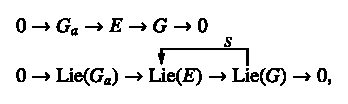
\includegraphics[scale=1.05]{chap6/fig7.eps}
\end{figure}
extend scalars from $R$ to $K=R\otimes Q$. Because $K$ is a $Q$-algebra, the Lie functor defines an equivalence of categories between commutative formal Lie groups over $K$ and free finitely generated $K$-modules.

Therefore there is a unique splitting as $K$-groups
\begin{figure}[H]
\centering
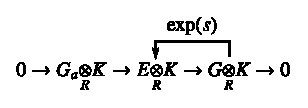
\includegraphics[scale=1.05]{chap6/fig8.eps}
\end{figure}
whose differential is the given splitting $S$ on Lie algebras.

At the same time, we may choose a cross section $S$ in the category of {\em pointed} f.p.p.f. sheaves over $R$
\begin{figure}[H]
\centering
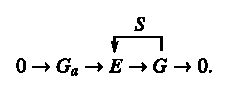
\includegraphics[scale=1.05]{chap6/fig9.eps}
\end{figure}

The difference $f=S-\exp(s)$ is a pointed map from $G\otimes K$ to $(G_{a})\otimes K$, i.e. an element $f\in A(G\otimes K)$, and it satisfied $f(0)=0$. We have $df=dS-s$, so $df$ is integral, and the formula
$$
f(X{\displaystyle{\mathop{+}\limits_{G}}}Y)-f(X)-f(Y)=S(X{\displaystyle{\mathop{+}\limits_{G}}}Y)-S(X)-s(Y),
$$
valid because $\exp(s)$ is a homomorphism, shows that $f(X{\displaystyle{\mathop{+}\limits_{G}}}Y)-f(X)-f(Y)$ is integral.

Because the initial choice of $S$ is indeterminate up to addition of a pointed map from $G$ to $G_{a}$, the class of $f=S-\exp (s)$ in $D(G/R)$ is well-defined independently of the choice of $S$, and it vanishes if and only if $\exp(s)$ is itself integral, i.e. if and only if the original rigidified extension is trivial as a rigidified extension. Thus we obtain an injective map
$$
\Ext^{\text{rigid}}(G,G_{a})\to D(G/R).
$$

To\pageoriginale see that it is an isomorphism, note that in any case the map $D(G/R)\to \Ext(G,G_{a})$ defined by $f\to$ the class of $\partial f$ sits in an exact sequence
$$
0\to \Hom(G,G_{a})\to \underline{\omega}_{G}\to D(G/R)\to \Ext(G,G_{a}),
$$
which receives the $\Ext^{\text{rigid}}$ exact sequence:
\[
\xymatrix@C=.5cm{
0\ar[r] & \Hom(G,G_{a})\ar@{=}[d]\ar[r] & \underline{\omega}_{G}\ar@{=}[d]\ar[r] & D(G/R)\ar[r] & \Ext(G,G_{a})\ar@{=}[d] &\\
0\ar[r] & \Hom(G,G_{a})\ar[r] & \underline{\omega}_{G}\ar[r] & \Ext^{\text{rigid}}(G,G_{a})\ar@{^(->}[u]\ar[r] & \Ext(G,G_{a})\ar[r] & 0
}
\]
The result is now visible.
\end{proof}

Given an ideal $I\subset R$, we denote by $\Ext(G,G_{a};I)$ the group of isomorphism classes of pairs consisting of an extension of $G$ by $G_{a}$ together with a splitting of its reduction modulo $I$. We denote by $\Ext^{\text{rigid}}(G,G_{a};I)$ the group of isomorphism classes of pairs consisting of a rigidified extension and a splitting of the reduction mod $I$ of the underlying extension. Analogously to the previous theorem, we have

\medskip
\noindent
{\bf Theorem \thnum{5.2.2}.\label{art6-thm5.2.2}}~{\em If $R$ is flat over $Z$, and $I\subset R$ an ideal, there is a natural isomorphism}
$$
\Ext^{\text{rigid}}(G,G_{a};I)\xrightarrow{\sim}D_{1}(G/R)
$$
{\em and a four-term exact sequence}
$$
0\to \Hom(G,G_{a})\to \underline{\omega}_{G}\to D_{1}(G/R)\xrightarrow{\partial}\Ext(G,G_{a};I)\to 0
$$
{\em in which the map $\partial$, given by}
\begin{gather*}
f\to \text{~the class of the symmetric 2-cocycle}\\[3pt]
\partial f=f(X{\displaystyle{\mathop{+}\limits_{G}}}Y)-f(X)-f(Y),
\end{gather*}
{\em corresponds to the map ``forget the rigidification'' on $\Ext$'s.}

\subsection{The Case of $p$-Divisible Formal Groups}\label{art6-sec5.3}
Let $p$ be a prime number. A ring $R$ is said to be $p$-adic if it is complete and separated in its $p$-adic topology, i.e., if
$$
R\xrightarrow{\sim} \varprojlim R/p^{n}R.
$$
A\pageoriginale commutative formal Lie group $G$ over a $p$-adic ring $R$ is said to be $p$-divisible of height $h$ if the map `multiplication by $p$'' makes $A(G)$ into a finite locally free module over itself of rank $p^{h}$.

If we denote by $G^{v}$ the dual of $G$ in the sense of $p$-divisible groups, it makes sense to speak of the tangent space of $G^{v}$ at the origin, noted $\underline{t}_{G^{v}}$; it is known that $\underline{t}_{G^{v}}$ is a locally free $R$-module of rank $h-\dim (G)$, and that there is a canonical isomorphism
\begin{equation*}
\Ext(G,G_{a})\xrightarrow{\sim}\underline{t}_{G^{v}}.\tag{5.3.1}\label{art6-eq5.3.1}
\end{equation*}
Because $G$ is $p$-divisible and $R$ is $p$-adic, $\Hom(G,G_{a})=0$, and the four-term exact sequence becomes a Hodge-like exact sequence
\begin{equation*}
0\to \underline{\omega}_{G}\to D(G/R)\to \underline{t}_{G^{v}}\to 0\tag{5.3.2}\label{art6-eq5.3.2}
\end{equation*}
Thus we find

\medskip
\noindent
{\bf Theorem \thnum{5.3.3}.\label{art6-thm5.3.3}}
\begin{itemize}
\item[(1)] {\em If $R$ is a $p$-adic ring which is flat over $Z$, then for a $p$-divisible commutative formal Lie group $G$ over $R$, the $R$-module $D(G/R)$ is locally free of rank $h=$ height $(G)$, and its formation commutes with arbitrary extension of scalars of $Z$-flat $p$-adic rings.}
\end{itemize}

If an addition $I\subset R$ is an ideal which is closed in the $p$-adic topology, then $R/I$ is again a $p$-adic ring, $G\otimes (R/I)$ is still $p$-divisible, and therefore admits no non-trivial homomorphisms to $G_{a}$ over $R/I$. It follows that 
\begin{equation*}
\begin{cases}
D_{1}(G/R)\subset D(G/R)\\[3pt]
\Ext(G,G_{a};I)\xrightarrow{I}I \Ext(G,G_{a})\simeq I\cdot \underline{t}_{G^{v}}
\end{cases}\tag{5.3.4}\label{art6-eq5.3.4}
\end{equation*}
and we have a short exact sequence
\begin{equation*}
0\to \underline{\omega}_{G}\to D_{1}(G/R)\to I\cdot \underline{t}_{G^{v}}\to 0.\tag{5.3.5}\label{art6-eq5.3.5}
\end{equation*}

\setcounter{subsection}{4}
\subsection{Relation to the Classical Theory}\label{art6-eq5.5}
Let $k$ be a perfect field of characteristic $p>0$, and take $R=W(k)$, $I=(p)$. Let $CW$ denote the $k$-group-functor ``Witt covectors'' (in the notations of Fontaine (\cite{art6-key13}), with its structure of $W(k)$-module. According to Fontaine, for any formal Lie variety $V$ over $W(k)$, we obtain a $W(k)$-linear isomorphism
\begin{equation*}
w:CW(A(V\otimes k))\xrightarrow{\sim}H^{1}_{\DR}(V/W(k);(p))\tag{5.5.1}\label{art6-eq5.5.1}
\end{equation*}
by\pageoriginale defining
\begin{equation*}
w(\ldots,a_{-a},\ldots,a_{0})=d\left(\sum\limits_{n\geq 0}\frac{(\widetilde{a}_{-a})^{p^{n}}}{p^{n}}\right)\tag{5.5.2}\label{art6-eq5.5.2}
\end{equation*}
where $\widetilde{a}_{-n}$ denotes an arbitrary lifting to $A(V)$ of $a_{-n}\in A(V\otimes k)$. Similarly, we can define, following Grothendieck, Mazur-Messing (\cite{art6-key35}), a $\sigma$-linear isomorphism
\begin{equation*}
\psi:CW(A(V\otimes k))\xrightarrow{\sim}H^{1}_{\DR}(V/W(k))\tag{5.5.3}\label{art6-eq5.5.3}
\end{equation*}
by the formula
\begin{equation*}
\psi(\ldots,a_{-n},\ldots,a_{0})=d\left(\sum\limits_{n\geq 0}\frac{(\widetilde{a}_{-n})^{p^{n+1}}}{p^{n+1}}\right).\tag{5.5.4}\label{art6-eq5.5.4}
\end{equation*}
These isomorphisms sit in a commutative diagram
\begin{equation*}
\vcenter{
\xymatrix@C=2cm{
 & H^{1}_{DR}(V/W(k);(p))\ar[dd]_-{\rotatebox{90}{$\sim$}}^-{\frac{1}{p}F}\\
CW(A(V\otimes k))\ar[dr]^-{\sim}_-{\psi} \ar[ur]^-{\sim}_-{w} &\\
 & H^{1}_{\DR}(V/W(k)).
}}\tag{5.5.5}\label{art6-eq5.5.5}
\end{equation*}

When $G$ is a commutative formal Lie group over $W(k)$ which is $p$-{\em divisible}, the ``classical'' Dieudonne module of $G_{0}=G\otimes k$ is {\em defined} as
\begin{equation*}
\vcenter{
\xymatrix@C=.1cm{
M(G_{0})\ar@{=}[r]^-{\text{dfn}} & \Hom_{k-gp}(G_{0},CW)\ar@{=}[d]\\
 & \text{the primitive elements in $CW(A(G_{0}))$.}
}}\tag{5.5.6}\label{art6-eq5.5.6}
\end{equation*}
Combining this definition with the previous isomorphisms, we find a commutative diagram of isomorphisms
\begin{equation*}
\vcenter{
\xymatrix@C=2cm{
 & D_{p}(G/W(k))\ar[dd]_-{\rotatebox{90}{$\sim$}}^-{\frac{1}{p}F}\\
M(G_{0})\ar[dr]^-{\sim}_-{\psi} \ar[ur]^-{\sim}_-{w} &\\
 & D(G/W(k)).
}}\tag{5.5.7}\label{art6-eq5.5.7}
\end{equation*}

\subsection{Relation with Abelian Schemes and with the General Theory}\label{art6-sec5.6}\pageoriginale
In this section, we recall without proofs some of the main results and compatibilities of the general $D$-theory of Grothendieck and Mazur-Messing.

Given an abelian scheme $A$ over an arbitrary ring $R$, there are canonical isomorphisms
\begin{equation*}
\begin{cases}
\Ext^{\text{rigid}}(A,G_{a})\xrightarrow{\sim}H^{1}_{\DR}(A/R)\\
\Ext(A,G_{a})\xrightarrow{\sim}H^{1}(A,O_{A})=\Lie(A^{v})
\end{cases}\tag{5.6.1}\label{art6-eq5.6.1}
\end{equation*}
in terms of which the $\Ext^{\text{rigid}}$-exact sequence ``becomes'' the Hodge exact sequence:
\begin{equation*}
\vcenter{
\xymatrix{
0\ar[r] & \underline{\omega}_{A}\ar[r]\ar@{=}[d] & \Ext^{\text{rigid}}(A,G_{a})\ar[d]_{\rotatebox{90}{$\sim$}}\ar[r] & \Ext(A,G_{a})\ar[d]_{\rotatebox{90}{$\sim$}}\ar[r] & 0\\
0\ar[r] & \underline{\omega}_{A}\ar[r] & H^{1}_{\DR}(A/R)\ar[r] & H^{1}(A,O_{A})\ar@{=}[d]\ar[r] & 0\\
        &                             &                      & \Lie(A^{v}) &    
}}\tag{5.6.2}\label{art6-eq5.6.2}
\end{equation*}

Given a $p$-divisible (Barsotti-Tate) group $G=\varinjlim G_{n}$ over a ring $R$ in which $p$ is nilpotent, the exact sequence
\begin{equation*}
0\to G_{n}\to G\xrightarrow{p^{n}}G\to 0\tag{5.6.3}\label{art6-eq5.6.3}
\end{equation*}
for any $n$ sufficiently large that $p^{n}=0$ in $R$, leads to a canonical isomorphism
\begin{equation*}
\Lie(G^{v})=\Lie(G^{v}_{n})=\Hom(G_{n},G_{a})\xrightarrow{\sim}\Ext(G,G_{a}).\tag{5.6.4}\label{art6-eq5.6.4}
\end{equation*}
The $\Ext^{\text{rigid}}$-exact sequence can thus be written
\begin{equation*}
0\to \underline{\omega}_{G}\to \Ext^{\text{rigid}}(G,G_{a})\to \Lie(G^{v})\to 0,\tag{5.6.5}\label{art6-eq5.6.5}
\end{equation*}
where $\underline{\omega}_{G}$ is the $R$-linear dual of $\Lie (G)$.

Given an abelian scheme $A$ over a ring $R$ in which $p$ is nilpotent, the exact sequence
\begin{equation*}
0\to A_{p^{n}}\to A\xrightarrow{p^{n}}\to A\to 0\tag{5.6.6}\label{art6-eq5.6.6}
\end{equation*}
for\pageoriginale any $n$ sufficiently large that $p^{n}=0$ in $R$ leads to a canonical isomorphism
\begin{equation*}
\Lie(A^{v})=\Lie(A^{v}_{p^{n}})=\Hom(A_{p^{n}},G_{a})\xrightarrow{\sim}\Ext(A,G_{a}).\tag{5.6.7}\label{art6-eq5.6.7}
\end{equation*}
Therefore the inclusion $A_{p^{\infty}}\hookrightarrow A$ induces an isomorphism
\begin{equation*}
\Ext(A,G_{a})\xrightarrow{\sim}\Ext(A_{p^{\infty}},G_{a})\tag{5.6.8}\label{art6-eq5.6.8}
\end{equation*}
(the identity on $\Hom(A_{p^{n}},G_{a})!$), and consequently we obtain a commutative diagram of isomorphisms
\begin{equation*}
\vcenter{
\xymatrix{
0\ar[r] & \underline{\omega}_{A}\ar@{=}[d]\ar[r] & \Ext^{\text{rigid}}(A,G_{a})\ar[d]_{\rotatebox{90}{$\sim$}}\ar[r] & \Ext(A,G_{a})\ar[d]_{\rotatebox{90}{$\sim$}}\ar[r] & 0\\
0\ar[r] & \underline{\omega}_{A_{p^{\infty}}}\ar[r] & \Ext^{\text{rigid}}(A_{p^{\infty}},G_{a})\ar[r] & \Ext(A_{p^{\infty}},G_{a})\ar[r] & 0,
}}\tag{5.6.9}\label{art6-eq5.6.9}
\end{equation*}
i.e., an isomorphism
\begin{equation*}
H^{1}_{\DR}(A/R)\xrightarrow{\sim}D(A_{p^{\infty}}/R)\tag{5.6.10}\label{art6-eq5.6.10}
\end{equation*}
compatible with the Hodge filtration.

For variable $B-T$ groups $G$ over a fixed ring $R$ in which $p$ is nilpotent, the functors $\underline{\omega}_{G}$, $\Lie(G^{v})$, and consequently $\Ext^{\text{rigid}}(G,G_{a})$, are exact functors whose values are locally free $R$-modules of finite rank; their formation commutes with arbitrary extension of scalars of rings in which $p$ is nilpotent.

Following Grothendieck and Mazur-Messing we {\em define}
\begin{equation*}
\vcenter{
\xymatrix{
D(G/R)\ar@{=}[r]^{\text{dfn}} & \Ext^{\text{rigid}}(G,G_{a})
}}\tag{5.6.11}\label{art6-eq5.6.11}
\end{equation*}
when $G$ is a $B-T$ group over a ring $R$ in which $p$ is nilpotent.

When $R$ is a $p$-adic ring, and $G$ is a $B-T$ group over $R$, we {\em define}
\begin{equation*}
\left\{
\begin{array}{r@{~=~}l}
D(G/R) & \varprojlim\limits_{n} D(G\otimes (R/p^{n}R)/(R/p^{n}R))\\[2pt]
\Lie(G) & \varprojlim \Lie (G\otimes (R/p^{n}R))\\[4pt]
\underline{\omega}_{G} & \varprojlim \underline{\omega}_{G}\otimes (R/p^{n}R)
\end{array}
\right.\tag{5.6.12}\label{art6-eq5.6.12}
\end{equation*}

Thus\pageoriginale for variable $B-T$ groups $G$ over a $p$-adic ring $R$, the functors $\underline{\omega}_{G}$, $\Lie(G^{v})$ and $D(G/R)$ are all exact functors in locally free $R$-modules of finite rank, sitting in an exact sequence
\begin{equation*}
0\to \underline{\omega}_{G}\to D(G/R)\to \Lie(G^{v})\to 0\tag{5.6.13}\label{art6-eq5.6.13}
\end{equation*}
whose formation commutes with arbitrary extension of scalars of $p$-adic rings. When $A$ is an abelian scheme over a $p$-adic ring $R$, we obtain an isomorphism
$$
H^{1}_{\DR}(A/R)\xrightarrow{\sim} D(A(p^{\infty})/R),
$$
compatible with Hodge filtrations, by passage to the limit.

As we have seen in the previous section, this general $\Ext^{\text{rigid}}$ notion of $D(G/R)$ agrees with our more explicit one in the case that both are defined, namely when $G$ is a $p$-divisible formal group over a $Z$-flat $p$-adic ring $R$.

\subsection{Relation with Cohomology}\label{art6-sec5.7}
~

\smallskip
\noindent
{\bf Theorem \thnum{5.7.1}.\label{art6-thm5.7.1}}~{\em Let $A$ be an abelian scheme over the Witt vectors $W(k)$ of an algebraically closed field $k$ of characteristic $p>0$. There is a short exact sequence of $W$-modules}
$$
0\to H^{1}_{\text{et}}(A\otimes k,Z_{p})\otimes W\xrightarrow{\alpha} H^{1}_{\text{cris}}(A\otimes k/W)\xrightarrow{\beta}D(\widehat{A}/W)\to 0
$$
{\em which is functorial in $A\otimes k$.}
\smallskip

\begin{proof}
We begin by defining the maps $\alpha$ and $\beta$. They will be defined by passage to the limit from maps $\alpha_{n}$, $\beta_{n}$ in an exact sequence
\begin{gather*}
0\to H^{1}_{\text{et}}(A\otimes k,Z/p^{n}Z)\otimes W_{n}\xrightarrow{\alpha_{n}}H^{1}_{\text{cris}}(A\otimes k/W_{n})\tag{5.7.2}\label{art6-eq5.7.2}\\
\xrightarrow{\beta_{n}}D(\widehat{A}\otimes W_{n}/W_{n})\to 0.
\end{gather*}
of $W_{n}$-modules.

An element of $H^{1}(A\otimes k, Z/p^{n}Z)$ is (the isomorphism class of) a $Z/p^{n}Z$-torsor over $A\otimes k$. An element of $H^{1}_{\text{cris}}(A\otimes k/W_{n})$ is (the isomorphism class of) a rule which assigns to every test situation $Y\hookrightarrow Y_{n}$\pageoriginale consisting an $A\otimes k$ scheme $Y$ and a divided-power thickening of $Y$ to a $W_{n}$-scheme $Y_{n}$ a $G_{a}$-torsor on $Y_{n}$ in a way which is compatible with inverse image whenever we have a morphism $(Y,Y_{n})\to (Y',Y'_{n})$ of such test situations (cf. \cite{art6-key35} for more details).

Given a $Z/p^{n}Z$-torsor $T$ on $A\otimes k$, we must define for every test situation $Y\hookrightarrow Y_{n}$, a $G$-torsor $\alpha_{n}(T)_{(Y,Y_{n})}$ on $Y_{n}$. Because $Y$ is given as an $A\otimes k$ scheme, we can pull back $T$ to obtain a $Z/p^{n}Z$-torsor $T_{Y}$ on $Y$. Because $Y_{n}$ is a $W_{n}$-scheme which is a divided-power thickening, its ideal of definition is necessarily a nil-ideal; therefore the etale $Y$-scheme $T_{Y}$ extends uniquely to an etale $Y_{n}$-scheme $T_{(Y,Y_{n})}$, and its structure of $Z/p^{n}Z$-torsor extends uniquely as well. Because $Y_{n}$ is a $W_{n}$-scheme, the natural map
$$
Z/p^{n}Z\to W_{n}
$$
gives rise to a morphism of algebraic groups on $Y_{n}$
$$
(Z/p^{n}Z)_{Y_{n}}\xrightarrow{\alpha_{n}}(G_{a})_{Y_{n}};
$$
the required $G_{a}$-torsor $\alpha_{n}(T)_{(Y,Y_{n})}$ is obtained by ``extension of structural groups via $\alpha_{n}$'' from the $Z/p^{n}$ $Z$-torsor $T_{(Y,Y_{n})}$.

To define $\beta_{n}$, we begin with an element $Z$ of $H^{1}_{\text{cris}}(A\otimes k/W_{n})$. We must define an element $\beta_{n}(Z)$ in $\Ext^{\text{rigid}}(\widehat{A}\otimes W_{n},(G_{a})\otimes W_{n})=D(\widehat{A}\otimes W_{n}/W_{n})$. Its value on the test object $A\otimes k\hookrightarrow A\otimes W_{n}$ is a $G_{a}$-torsor on $A\otimes W_{n}$ which is endowed with an integrable connection (cf. \cite{art6-key2}, \cite{art6-key3}), i.e., it is an element of $H^{1}_{\DR}(A\otimes W_{n}/W_{n})$. [This interpretation provides the canonical isomorphism
$$
H^{1}_{\text{cris}}(A\otimes k/W_{n})\xrightarrow{\sim}H^{1}_{\DR}(A\otimes W_{n}/W_{n}).]
$$
Composing with the isomorphism
$$
H^{1}_{\DR}(A\otimes W_{n}/W_{n})\xrightarrow{\sim}\Ext^{\text{rigid}}(A\otimes W_{n},G_{a}\otimes W_{n}),
$$
we obtain an element of $\Ext^{\text{rigid}}(A\otimes W_{n},G_{a}\otimes W_{n})$, whose restriction to the formal group $\widehat{A}\otimes W_{n}$ is the required element $\beta_{n}(Z)$.

To see that the map $\beta$ obtained from these $\beta_{n}$ by passage to the limit is\pageoriginale in fact functorial in $A\otimes k$, we first note that it sits in the commutative diagram
\begin{equation*}
\vcenter{
\xymatrix@C=2cm@R=1.5cm{
H^{1}_{\text{cris}}(A\otimes k/W)\ar[d]_-{\rotatebox{90}{$\backsim$}}^-{\text{canonical isom}}\ar[r]^-{\beta} & D(\widehat{A}/W)\ar@{_(->}[d]^{\substack{\text{inclusion of}\\ \text{primitive}\\ \text{elements}}}\\
H^{1}_{\DR}(A/W)\ar[r]^-{\text{natural map}}_-{\text{``restriction to $\widehat{A}$''}} & H^{1}_{\DR}(\widehat{A}/W).
}}\tag{5.7.3}\label{art6-eq5.7.3}
\end{equation*}

What must be shown is that if we are given a second abelian scheme $B$ over $W$, and a homomorphism
$$
f_{0}:B\otimes k\to A\otimes k
$$
then the diagram
\begin{equation*}
\vcenter{
\xymatrix@C=2cm@R=1.5cm{
H^{1}_{\text{cris}}(A\otimes k/W) \ar[r]^-{\beta} \ar[d]^-{(f_{0})^{*}} & D(\widehat{A}/W)\ar[d]^-{\substack{\text{(any pointed}\\ \text{lifting of $\widehat{f}_{0}$)$^{*}$}}}\\
H^{1}_{\text{cris}}(B\otimes k/W)\ar[r]^-{\beta} & D(\widehat{B}/W)
}}\tag{5.7.4}\label{art6-eq5.7.4}
\end{equation*}
is {\em commutative}.

But in virtue of the commutativity of the previous diagram \eqref{art6-eq5.7.3}, it is enough to show the commutativity of the diagram
\begin{equation*}
\vcenter{
\xymatrix@C=2cm@R=1.5cm{
H^{1}_{\text{cris}}(A\otimes k/W)\simeq H^{1}_{\DR}(A/W) \ar[r]^-{\text{restriction}} \ar[d]^-{(f_{0})^{*}} & H^{1}_{\DR}(\widehat{A}/W)\ar[d]^-{\substack{\text{(any pointed}\\ \text{lifting of $\widehat{f}_{0}$)$^{*}$}}}\\
H^{1}_{\text{cris}}(B\otimes k/W)\simeq H^{1}_{\DR}(B/W) \ar[r]^-{\text{restriction}} & H^{1}_{\DR}(\widehat{B}/W).
}}\tag{5.7.5}\label{art6-eq5.7.5}
\end{equation*}

This\pageoriginale last commutativity has nothing to do with abelian schemes, nor does it require pointed liftings. It is an instance of the following general fact, whose proof we defer for a moment.

\medskip
\noindent
{\bf General Fact \thnum{5.7.6}.\label{art6-5.7.6}}~{\em For any two pointed $W$-schemes $A$, $B$ which are both proper and smooth, any pointed map $f_{0}:B\otimes k\to A\otimes k$, and any integer $i\geq 0$, we have a commutative diagram}
\begin{equation*}
\xymatrix@C=2cm@R=1.5cm{
H^{1}_{\text{cris}}(A\otimes k/W)\sim H^{i}_{\DR}(A/W) \ar[r]^-{\text{restriction}} \ar[d]^-{(f_{0})^{*}} & H^{i}_{\DR}(\widehat{A}/W)\ar[d]^-{\substack{\text{(any lifting}\\ \text{of $\widehat{f}_{0}$)$^{*}$}}}\\
H^{1}_{\text{cris}}(B\otimes k/W)\simeq H^{i}_{\DR}(B/W)\ar[r]^-{\text{restriction}} & H^{i}_{\DR}(\widehat{B}/W)
}
\end{equation*}

To conclude the proof of the theorem (!), it remains to see that our marvelously functorial maps $\alpha$, $\beta$ really do form an exact sequence. To do this, we will use the abelian scheme $A$ over $W$. Its formal group $\widehat{A}$ is $p$-divisible, and sits in an exact sequence of $p$-divisible groups over $W$,
$$
0\to \widehat{A}_{p^{\infty}}\to A_{p^{\infty}}\to E\to 0,
$$
in which $E=\varinjlim E_{n}$ denote the etale quotient of $A_{p^{\infty}}$. Because $k$ is algebraically closed, $E$ is a {\em constant} $p$-divisible group, namely the abstract $p$-divisible group $\varinjlim A_{p^{n}}(k)$ of all $p$-power torsion points of $A(k)$.

We will identify the exact sequence of the proposition with the exact sequence
$$
0\to D(E/W)\xrightarrow{\alpha'}D(A_{p^{\infty}}/W)\xrightarrow{\beta'}D(\widehat{A}/W)\to 0,
$$
and we will identify the $(\alpha_{n},\beta_{n})$-sequence with the exact sequence
$$
0\to D(E\otimes W_{n}/W_{n})\xrightarrow{\alpha'_{n}}D(A_{p^{\infty}}\otimes W_{n}/W_{n})\xrightarrow{\beta'_{n}}D(\widehat{A}\otimes W_{n}/W_{n})\to 0.
$$

It\pageoriginale is clear from the construction of $\beta_{n}$ that we have a commutative diagram
\[
\xymatrix@C=1.5cm{
D(A_{p^{\infty}}\otimes W_{n}/W_{n})\ar@{=}[d]\ar[r]^-{\beta'_{n}} & D(\widehat{A}\otimes W_{n}/W_{n})\ar@{=}[d]^-{\text{dfn}}\\
\Ext^{\text{rigid}}(A_{p^{\infty}}\otimes W_{n},G_{a})\ar[r]^-{\text{restriction}} & \Ext^{\text{rigid}}(\widehat{A}\otimes W_{n},G_{a})\\
\Ext^{\text{rigid}}(A\otimes W_{n},G_{a})\ar[u]^{\rotatebox{90}{$\backsim$}}\ar[d]_{\rotatebox{90}{$\backsim$}}\ar[ur]^-{\text{restriction}}  &\\
H^{1}_{\DR}(A\otimes W_{n}/W_{n}) &\\
H^{1}_{\text{cris}}(A\otimes k/W_{n}).\ar[u]^{\rotatebox{90}{$\backsim$}} \ar[uuur]_{\beta_{n}}
}
\]

To relate the map $\alpha_{n}$ to the $D$-maps, use the exact sequence
$$
0\to E_{n}\otimes W_{n}\to E\otimes W_{n}\xrightarrow{p^{n}} E\otimes W_{n}\to 0
$$
to compute
\[
\xymatrix@C=.5cm{
D(E\otimes W_{n}/W_{n})\ar[r]^{\sim} & \Ext(E\otimes W_{n},G_{a})\ar[r]^{\sim} & \Hom(E_{n}\otimes W_{n},G_{a})\ar[d]_{\rotatebox{90}{$\backsim$}}^-{(E_{n}\text{~ is constant})}\\
 & & \Hom(E_{n}(W_{n}),G_{a}(W_{n}))\ar@{=}[d]\\
 & & \Hom(E_{n}(k),W_{n})\ar@{=}[d]\\
 & & \Hom(E_{n}(k),Z/p^{n}Z)\otimes W_{n}.
}
\]
Next use the sequence
$$
0\to A_{p^{n}}\otimes W_{n}\to A\otimes W_{n}\xrightarrow{p^{n}} A\otimes W_{n}\to 0
$$
to\pageoriginale compute
\[
\xymatrix{
\Ext(A\otimes W_{n}, Z/p^{n}Z)\ar[r]^-{\sim} & \Hom(A_{p^{n}}\otimes W_{n},Z/p^{n}Z)  \\
 & \Hom(E_{n}\otimes W_{n},Z/p^{n}Z)\ar[u]^{\rotatebox{90}{$\backsim$}}_{(E_{n} = \text{~etale quotient of $A_{p^{n}}$})}\ar[d]_{\rotatebox{90}{$\backsim$}}\\
H^{1}_{\text{et}}(A\otimes k, Z/p^{n}Z) & \Hom(E_{n}(k),Z/p^{n}Z).\ar[l]_{\sim} 
}
\]
Combining these isomorphisms, and remembering that 
$$
\Ext=\Ext^{\text{rigid}}
$$ 
when either of the arguments is etale, we find a commutative diagram
\[
\xymatrix{
D(E\otimes W_{n}/W_{n})\ar[r]^-{\alpha'_{n}} & D(A_{p^{\infty}}\otimes W_{n}/W_{n})\\
\Hom(E_{n}(k),Z/p^{n}Z)\otimes W_{n}\ar[u]^{\rotatebox{90}{$\backsim$}} & D(A\otimes W_{n}/W_{n})\ar[u]^{\rotatebox{90}{$\backsim$}}\\
\Ext^{\text{rigid}}(A\otimes W_{n},Z/p^{n}Z)\otimes W_{n}\ar[r]^{*{*}*}\ar[u]^{\rotatebox{90}{$\backsim$}} & \Ext^{\text{rigid}}(A\otimes W_{n},G_{a})\ar@{=}[u]\\
H^{1}_{\text{et}}(A\otimes k, Z/p^{n}Z)\otimes W_{n}\ar[u]^{\rotatebox{90}{$\backsim$}}\ar[r]^-{\alpha_{n}} & H^{1}_{\text{cris}}(A\otimes k/W_{n})\ar@{=}[u]
}
\]
in which the arrow ${*}{*}{*}$ is ``push-out'' along the homomorphism
$$
Z/p^{n}Z\to W_{n}\to (G_{a})_{W_{n}}.
$$
\end{proof}

\medskip
\noindent
{\bf Corollary \thnum{5.7.7}.\label{art6-coro5.7.7}}~{\em Let $A$ be an abelian scheme over the Witt vectors $W(k)$ of a perfect field $k$ of characteristic $p>0$. Then we have a short exact sequence of $W(k)$-modules}
\begin{align*}
0\to &\left((H^{1}_{\text{et}}(A\otimes \overline{k},Z_{p})\otimes W(\overline{k})\right)^{\Gal(\overline{k}/k)}\to\\
& H^{1}_{\text{cris}}(A\otimes k/W(k))\to D(\widehat{A}/W(k))\to 0,
\end{align*}
{\em in which $\overline{k}$ denotes an algebraic closure of $k$, and in which the galois group $\Gal(\overline{k}/k)$ acts simultaneously on $H^{1}_{\text{et}}(A\otimes \overline{k},Z_{p})$ and on $W(\overline{k})$ by ``transport of structure''.}

\begin{proof}
One\pageoriginale can obtain this sequence either by passing to $\Gal(\overline{k}/k)$-in\-variants in the already-established analogous sequence for $A\otimes W(\overline{k})$, or by repeating the {\em proof} given for the proposition. In the latter case, one finds, in the notations of the proof,
\begin{align*}
D(E\otimes W_{n}(k)/W_{n}(k)) &\simeq \Hom(E_{n}\otimes W_{n}(k),(G_{a})_{W_{n}(k)})\\[3pt]
&\simeq \Hom(E_{n}(\overline{k}),W_{n}(\overline{k}))^{\Gal(\overline{k}/k)}\\[3pt]
&\simeq \Hom(A_{p^{n}}(\overline{k}), W_{n}(\overline{k}))^{\Gal(\overline{k}/k)}\\[3pt]
&= \left(H^{1}_{\text{et}}(A\otimes \overline{k},Z/p^{n}Z)\otimes W_{n}(\overline{k})\right)^{\Gal(\overline{k}/k)}
\end{align*}
and the rest of the proof remains unchanged.
\end{proof}

\medskip
\noindent
{\bf Corollary \thnum{5.7.8}.\label{art6-coro5.7.8}}~{\em Let $A$ be an abelian scheme over the Witt vectors of a perfect field $k$ of characteristic $p>0$. The above exact sequence is the Newton-Hodge filtration}
$$
0\to (\text{slope~}0)\to H^{1}_{\text{cris}}(A\otimes k/W)\to (\text{slope~}>0)\to 0
$$
{\em of $H^{1}_{\text{cris}}(A\otimes k/W)$) as an $F$-crystal.}
\smallskip

\begin{proof}
Since $F$ induces a $\sigma$-linear automorphism of
\begin{align*}
& (H^{1}_{\text{et}}(A\otimes \overline{k},Z_{p})\otimes W(\overline{k}))^{\Gal}\\[3pt]
& \simeq \left(\Hom(T_{p}(A\otimes \overline{k}),W(\overline{k}))\right)^{\Gal(\overline{k}/k)},
\end{align*}
it remains only to see that $F$ is topologically nilpotent on $D(\widehat{A}/W(k))$, for its $p$-adic topology. Because $D(\widehat{A}/W(k))$ is a {\em finitely generated} $W(k)$ sub-module of $H^{1}_{\DR}(\widehat{A}/W(k))$, the topology {\em induced} on $D(\widehat{A}/W(k))$ by the {\em inverse limit} topology on $H^{1}_{\DR}$ through the isomorphism (cf. lemma \ref{art6-lem5.8.1}. ahead)
\begin{equation*}
H^{1}_{\DR}(\widehat{A}/W(k))\xrightarrow{\sim} \varprojlim H^{1}_{\DR}(\widehat{A}\otimes W_{n}(k)/W_{n}(k))\tag{5.7.9}\label{art6-eq5.7.9}
\end{equation*}
must be {\em equivalent} to the $p$-adic topology in $D(\widehat{A}/W(k))$. So it suffices to remark that $F^{n}$ annihilates $H^{1}_{\DR}(\widehat{A}\otimes W_{n}/W_{n})$ (indeed $F^{n}$ annihilates $\Omega^{i}_{\widehat{A}\otimes W_{n}/W_{n}}$ for $i\geq 1$, since for any pointed lifting of $X\mapsto X^{p}$, $F(dX)=d(F(X))=d(X^{p}+pY)\in p\Omega^{1}$) to establish the required topological nilpotence of $F$ on $D(\widehat{A}/W)$. 
\end{proof}

\subsection{The Missing Lemmas}\label{art6-sec5.8}\pageoriginale
It remains for us to establish the ``general fact'' \eqref{art6-coro5.7.7}, and to establish the isomorphism \eqref{art6-eq5.7.9}. In fact, the two questions are intimately related. We begin with the second.

\medskip
\noindent
{\bf Lemma \thnum{5.8.1}.\label{art6-lem5.8.1}}~{\em Let $R$ be a $Z$-flat $p$-adic ring, and let $R_{n}=R/p^{n}R$. For any formal Lie variety $V$ over $R$, we have isomorphisms}
$$
H^{i}_{\DR}(V/R)\xrightarrow{\sim}\varprojlim H^{i}_{\DR}(V\otimes R_{n}/R_{n}).
$$

\begin{proof}
Pick coordinates $X_{1},\ldots,X_{N}$ for $V$. Over any ring $R$, we can define a $Z^{N}$-grading of the de Rham complex of $R[[X_{1},\ldots,X_{N}]]/R$, by attributing the weight $(a_{1},\ldots,a_{N})\in Z^{N}$ to each ``monomial''
$$
\left(\prod X^{a_{i}}_{i}\right)\left(\prod\limits_{j\in S}\frac{dX_{j}}{X_{j}}\right)\qquad S\text{~ any subset of~ }\{1,\ldots,N\}.
$$
Exterior differentiation is homogeneous of degree zero, and the de Rham complex is the {\em product} of all its homogeneous graded pieces
$$
\Omega^{\bigdot}=\Pi \Omega^{\bigdot}(a_{1},\ldots,a_{N}).
$$

Because both cohomology and inverse limits commute with products, we are reduced to proving the lemma homogeneous component by homogeneous component.

The individual complexes $\Omega^{\bigdot}(a_{1},\ldots,a_{N})$ are quite simple. They vanish except when all $a_{i}\geq 0$. The complex $\Omega^{\bigdot}(0,\ldots,0)$ is
$$
R\to 0\to 0\to \ldots
$$
If some $a_{i}\geq 1$, and all $a_{i}\geq 0$, the complex $\Omega^{\bigdot}(a_{1},\ldots,a_{N})$ is the tensor product complex
$$
\bigotimes\limits_{i\text{~with~}a_{i}\geq 1}\left(R\xrightarrow{a_{i}}R\right).
$$
What is important for us is that each of these complexes is obtained from a complex of free finitely generated $Z$-modules (!) by extension of scalars to $R$.

Thus let $K$ denote any complex of free finitely-generated $Z_{p}$-modules. We must show that for a $Z$-flat $p$-adic ring $R$ we have
$$
H^{i}(K^{\bigdot}\otimes R)\xrightarrow{\sim}\varprojlim H^{i}(K^{\bigdot}\otimes R_{n}).
$$
The\pageoriginale exact sequence of complexes
$$
0\to K^{\bigdot}\otimes R\xrightarrow{p^{n}} K^{\bigdot}\otimes R\to K^{\bigdot}\otimes R_{n}\to 0
$$
gives a ``universal coefficients'' exact sequence
$$
0\to H^{i}(K^{\bigdot}\otimes R)\otimes R_{n}\to H^{i}(K^{\bigdot}\otimes R_{n})\to p^{n}\text{-Torsion~}(H^{i+1}(K^{\bigdot}\otimes R))\to 0.
$$
Passing to the inverse limit over $n$ leads to an exact sequence
$$
0\to \varprojlim H^{i}(K^{\bigdot}\otimes R)\otimes R_{n}\to \varprojlim H^{i}(K^{\bigdot}\otimes R^{n})\to T_{p}(H^{i+1}(K^{\bigdot}\otimes R))\to 0.
$$

To see that $T_{p}(H^{i+1}(K^{\bigdot}\otimes R))$ vanishes, notice that an element of this $T_{p}$ is represented by a system of elements $a_{n}\in K^{i+1}\otimes R$ with $d(a_{n})=0$, $pa_{n+1}=a_{n}-d(b_{n})$, $a_{0}=0$; because both $K^{i}\otimes R$ and $K^{i+1}\otimes R$ are $p$-adically complete and separated, we may infer
\begin{align*}
a_{n} &= pa_{n+1}+d(b_{n})\\[3pt]
&= p\left(pa_{n+2}+d(b_{n+1})\right)+d(b_{n})\\[3pt]
&= \ldots\\[3pt]
&= d\left(\sum\limits_{i\geq 0}p^{i}b_{n+i}\right).
\end{align*}
To see that the natural map
$$
H^{i}(K^{\bigdot}\otimes R)\to \varprojlim H^{i}(K^{\bigdot}\otimes R)\otimes R_{n}
$$
is an isomorphism, use the $Z$-flatness of $R$ and the $Z$-finite generation of the $K^{i}$ to write
\begin{align*}
H^{i}(K^{\bigdot}\otimes R)\xleftarrow{\sim} H^{i}(K^{\bigdot})\otimes R &= (\text{fin. gen. $Z$-module})\otimes R\\[3pt]
&= \left(Z^{n}\oplus (\oplus Z/p^{n_{i}})\oplus \binom{\text{prime-to-$p$}}{\text{torsion}}\right)\otimes R\\[3pt]
&= R^{n}\oplus (\oplus R_{n_{i}}).
\end{align*}
\end{proof}

We now turn to the proof of the ``general fact''.

\medskip
\noindent
{\bf Lemma \thnum{5.8.2}.\label{art6-lem5.8.2}}~{\em Let $k$ be a perfect field of characteristic $p>0$, $A$ and $B$ two proper, smooth pointed $W(k)$-schemes, $f_{0}:B\otimes k\to A\otimes k$ a pointed $k$-morphism and $\widehat{f}:\widehat{B}\to \widehat{A}$ a $W$-lifting of $f_{0}$ to the formal completions\pageoriginale viewed as functors only on $p$-adic $W$-algebras. Then the diagram}
\[
\xymatrix@C=1.5cm{
H^{i}_{\text{cris}}(A\otimes k/W)\ar[d]^-{(f_{0})^{*}}\ar[r]^-{\sim} & H^{i}_{\DR}(A/W)\ar[r]^{\text{restriction}} & H^{i}_{\DR}(\widehat{A}/W)\ar[d]^-{(f)^{*}}\\
H^{i}_{\text{cris}}(B_{0}\otimes k/W)\ar[r]^-{\sim} & H^{i}_{\DR}(B/W)\ar[r]^-{\text{restriction}} & H^{i}_{\DR}(\widehat{B}/W)
}
\]
{\em is commutative}.
\smallskip

\begin{proof}
If $f_{0}$ lifted, this would be obvious. But it does lift locally, which is enough for us. More precisely, let $U\subset A$ and $V\subset B$ be affine open neighborhoods of the marked $W$-valued points of $A$ and $B$ respectively such that $f_{0}$ maps $V\otimes k$ to $U\otimes k$. Because $V$ is affine and $U$ is smooth over $W$, we may successively construct a compatible system of $W_{n}$-maps $f_{n}:V\otimes W_{n}\to U\otimes W_{n}$ with $f_{n+1}\equiv f_{n}\mod p^{n}$. The $f_{n}$ induce compatible maps $\widehat{f}_{n}:\widehat{B}\otimes W_{n}\to \widehat{A}\otimes W_{n}$ of formal completions, but these $\widehat{f}_{n}$ need {\em not} be {\em pointed} morphisms.

We denote by $\widehat{f}_{\infty}:\widehat{B}\to \widehat{A}$ the limit of these $\widehat{f}_{n}$. (Strictly speaking, $\widehat{f}_{\infty}$ only makes sense as a map of functors when we {\em restrict} $\widehat{B}$ and $\widehat{A}$ to the category of $p$-adic $W$-algebras).

For each $n$, we have a commutative diagram
\begin{figure}[H]
\centering
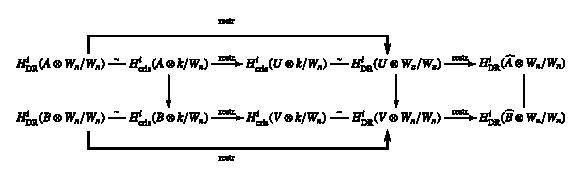
\includegraphics[scale=1.15]{chap6/fig10.eps}
\end{figure}
%\[
%\xymatrix{
%  H^{i}_{\DR}(A\otimes W_{n}/W_{n})\ar@{-}[r]^-{\sim} & H^{i}_{\text{cris}}(A\otimes k/W_{n})\ar[d]\ar[r]^{\text{restr.}} & H^{i}_{\text{cris}}(U\otimes k/W_{n})\ar@{-}[r]^-{\sim} & H^{i}_{\DR}(U\otimes W_{n}/W_{n})\ar[d]\ar[r]^-{\text{restr.}} & H^{i}_{\DR}(\widehat{A}\otimes W_{n}/W_{n})\ar[d]\\
% H^{i}_{\DR}(B\otimes W_{n}/W_{n})\ar@{-}[r]^-{\sim} & H^{i}_{\text{cris}}(B\otimes k/W_{n})\ar[r]^{\text{restr.}} & H^{i}_{\text{cris}}(V\otimes k/W_{n})\ar@{-}[r]^-{\sim} & H^{i}_{\DR}(V\otimes W_{n}/W_{n})\ar[r]^-{\text{restr.}} & H^{i}_{\DR}(\widehat{B}\otimes W_{n}/W_{n})\\
%}
%\]

Passing to the inverse limit over $n$, and using the previous lemma to identify the right-hand inverse limits, we obtain a commutative diagram
\[
\xymatrix@C=1.5cm{
H^{i}_{\text{cris}}(A\otimes k/W)\ar[d]^{(f_{0})^{*}}\ar@{-}[r]^-{\sim} & H^{i}_{\DR}(A/W)\ar[r]^-{\text{restriction}} & H^{i}_{\DR}(\widehat{A}/W)\ar[d]^-{(\widehat{f}_{\infty})^{*}}\\
H^{i}_{\text{cris}}(B\otimes k/W)\ar@{-}[r]^-{\sim} & H^{i}_{\DR}(\widehat{B}/W)\ar[r]^-{\text{restriction}} & H^{i}_{\DR}(\widehat{B}/W).
}
\]

To\pageoriginale conclude the proof, we need to know that the induced map
$$
(\widehat{f}_{\infty})^{*}:H^{i}_{\DR}(\widehat{A}/W)\to H^{i}_{\DR}(\widehat{B}/W)
$$
depends only on the underlying map $\widehat{f}_{0}:\widehat{B}\otimes k\to \widehat{A}\otimes k$, and not on the particular choice of lifting. In fact this is true for the individual $\widehat{f}_{n}$ as well!
\end{proof}

\medskip
\noindent
{\bf Lemma \thnum{5.8.3}.\label{art6-lem5.8.3}}~{\em Let $R$ be a $p$-adic ring. Let $V$ and $V'$ be formal Lie varieties over $R$, and let $f_{1}$ and $f_{2}$ be morphisms of functors $V'\to V$ of the restrictions of $V'$, $V$ to the category of $p$-adic $R$-algebras. If $f_{1} \ f_{2} \mod p$, then for each $i$, the induced maps}
$$
f^{*}_{1},f^{*}_{2}:H^{i}_{\DR}(V/R)\to H^{i}_{\DR}(V'/R)
$$
{\em are equal.}
\smallskip

\begin{proof}
(compare Monsky \cite{art6-key39}). In terms of coordinates $X_{1},\ldots,X_{n}$ for $V'$, $Y_{1},\ldots Y_{m}$ for $V$, the corresponding $R$-algebra homomorphisms
$$
\varphi_{1},\varphi_{2} : R[[Y_{1},\ldots,Y_{m}]]\to R[[X_{1},\ldots,X_{n}]]
$$
are related by
$$
\varphi_{2}(Y)=\varphi_{1}(Y)+p\Delta (Y).
$$
Introduce a new variable $T$, and consider the map 
\begin{gather*}
\varphi : R[[Y_{1},\ldots,Y_{m}]]\to R[[X_{1},\ldots,X_{n},T]]\\[3pt]
\varphi(Y)=\varphi_{1}(Y)+T\cdot \Delta(Y).
\end{gather*}
We have a commutative diagram of algebraic homomorphisms
\begin{figure}[H]
\centering
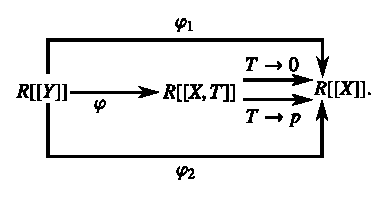
\includegraphics{chap6/fig11.eps}
\end{figure}
So\pageoriginale it suffices to consider the situation
\[
\xymatrix{
R[[X,T]]\ar@<.3em>[r]^-{T\to 0} \ar@<-.3em>[r]_-{T\to p} & R[[X]]
}
\]
and show that these two maps have the same effect on $H_{\DR}$.

A form $\omega$ on $R[[X,T]]$ may be written uniquely
$$
\omega = \sum\limits_{n\geq 0} a_{n}\cdot T^{n}+\sum\limits_{n\geq 1}b_{n}T^{n}\dfrac{dT}{T}
$$
with $a_{n}$, $b_{n}$'s forms on $R[[X]]$. This form is {\em closed} if and only if
$$
d(a_{n})=0\quad\text{for}\quad n\geq 0,\quad n\cdot a_{n}+d(b_{n})=0\quad \text{for}\quad n\geq 1.
$$

Its images under $T\to 0$ and $T\to p$ are
$$
a_{0},\quad \sum\limits_{n\geq 0} a_{n}p^{n}
$$
respectively. Their {\em difference}, if $\omega$ is closed, is exact, namely
$$
\omega|_{T=0}-\omega|_{T=p}=\sum\limits_{b\geq 1}a_{n}p^{n}=d\left(\sum\limits_{n\geq 1}\frac{p^{n}}{n}\cdot b_{n}\right).
$$
\end{proof}

It seems worthwile to point out that this last lemma can be considerably strengthened.

\medskip
\noindent
{\bf Lemma \thnum{5.8.4}.\label{art6-lem5.8.4}}~{\em Let $R$ be a $p$-adic ring, $I\subset R$ a divided power ideal, $V$ and $V'$ two formal Lie varieties over $R$, and $f_{1}$, $f_{2}$ two morphisms of functors $V'\to V$ of the restrictions of $V$, $V'$ to the category of $p$-adic $R$-algebras. If $f_{1}\equiv f_{2}\mod I$, then for all $i$ the induced maps}
$$
f^{*}_{1},f^{*}_{2} : H^{i}_{\DR}(V/R)\to H^{i}_{\DR}(V'/R)
$$
{\em are equal.}
\smallskip

\begin{proof}
If we had $f_{1}\equiv f_{2}\mod I'$ with $I'\subset I$ a {\em finitely generated} ideal, then we could repeat the proof of the previous lemma, introducing several new\pageoriginale variables $T_{i}$, one for each generator of $I'$. In particular, the lemma is true if $f_{1}$ and $f_{2}$ are {\em polynomial} maps in some coordinate system. But we easily reduce to this situation, for in terms of coordinates $X_{1},\ldots,X_{n}$ for $V'$, we have a $Z^{n}$-graduation of its de Rham complex and a corresponding product decomposition
$$
H^{i}_{\DR}(V'/R)=\prod\limits_{(a_{1},\ldots,a_{n})}H^{i}_{\DR}(V'/R)(a_{1},\ldots,a_{n}).
$$
Therefore it suffices to show that the composite maps
\[
\xymatrix@C=1.5cm{
H^{i}_{\DR}(V/R) \ar@<.3em>[r]^-{f^{*}_{1}} \ar@<-.3em>[r]_-{f^{*}_{2}} & H^{i}_{\DR}(V'/R)\ar[r]^-{\text{projection}} & H^{i}_{\DR}(V'/R)(a_{1},\ldots,a_{n})
}
\]
agree, for every $(a_{1},\ldots,a_{n})\in Z^{n}$. But for fixed $(a_{1},\ldots,a_{n})$, these composites depend only on the terms of total degree $\leq \sum a_{i}$ in the power series formulas for the maps $f_{1}$, $f_{2}$. Thus we are reduced to the case when $f_{1}$ and $f_{2}$ are each {\em polynomial} maps.
\end{proof}

\smallskip
\noindent
{\bf Remark \thnum{5.8.5}.\label{art6-rem5.8.5}}~If the ideal $I$ is closed, the proof gives the same invariance property for the groups $H^{i}_{\DR}(V/R;I)$ defined as the cohomology of
$$
``I\Omega^{i-1}_{V/R}\text{''} \xrightarrow{d}\Omega^{i}_{V/R}\xrightarrow{d}\Omega^{i+1}_{V/R}.
$$

\subsection{Application to the Cohomology of Curves}\label{art6-sec5.9}
Throughout this section we work over a mixed-characteristic valuation ring $R$ of residue characteristic $p$, which is complete for a rank-one (i.e., real-valued) valuation. Let $C$ be a projective smooth curve over $R$, with geometrically connected fibres of genus $g$. Its Jacobian $J=\Pic^{0}(C/R)$ is a $g$-dimensional autodual abelian scheme over $R$. For each rational point $x\in C(R)$, we denote by $\varphi_{x}$ the corresponding Albanese mapping 
$$
\varphi_{x} : C\to J
$$
given on $S$-valued points, $S$ any $R$-scheme, by
$$
\varphi_{x}(y)=\text{~the class of the invertible sheaf~}I(y)^{-1}\otimes I(x),
$$
where $I(y)$ denotes the invertible ideal sheaf of $y\in C(S)$ viewed as a Cartier\pageoriginale divisor in $C{\displaystyle{\mathop{\times}\limits_{R}}}S$. As is well-known (cf. \cite{art6-key44}, \cite{art6-key45}), this morphism induces isomorphisms
\begin{equation*}
\begin{cases}
H^{1}(J,O_{j})\xrightarrow{\sim} H^{1}(C,O_{C})\\[3pt]
H^{0}(J,\Omega^{1}_{J/R})=\underline{\omega}_{J}\xrightarrow{\sim}H^{0}(C,\Omega^{1}_{C/R})\\[3pt]
H^{1}_{\DR}(J/R)\xrightarrow{\sim} H^{1}_{\DR}(C/R)
\end{cases}\tag{5.9.1}\label{art6-eq5.9.1}
\end{equation*}
which are independent of the choice of the rational point $x$.

Let $\widehat{C}_{x}$ denote the formal completion of $C$ along $x$; it is a pointed formal Lie variety of dimension one over $R$. Because $\varphi_{X}(0)=0$, $\varphi_{x}$ induces a map of pointed formal Lie varieties
$$
\widehat{\varphi}_{x}:\widehat{C}_{x}\to \widehat{J},
$$
whence an induced map on cohomology
$$
D(\widehat{J}/R)\subset H^{1}_{\DR}(\widehat{J}/R)\xrightarrow{(\widehat{\varphi}_{x})^{*}}H^{1}_{\DR}(\widehat{C}_{x}/R).
$$

\medskip
\noindent
{\bf Theorem \thnum{5.9.2}.\label{art6-thm5.9.2}}~{\em The composite map}
$$
D(\widehat{J}/R)\xrightarrow{(\widehat{\varphi}_{x})^{*}}H^{1}_{\DR}(\widehat{C}_{x}/R)
$$
{\em is injective}.

\medskip
\noindent
{\bf Corollary \thnum{5.9.3}.\label{art6-coro5.9.3}}~{\em The natural map}
$$
H^{0}(C,\Omega^{1}_{C/R})\to H^{1}_{\DR}(\widehat{C}_{x}/R)
$$
{\em is injective, i.e., a non-zero differential of the first kind cannot be formally exact}.
\smallskip

\begin{proof}
Because $\widehat{J}$ is $p$-divisible, the natural map $\underline{\omega}_{J}\to D(J/R)$ is injective.

The corollary then follows immediately from the theorem and the commutativity of the diagram
\begin{equation*}
\vcenter{
\xymatrix@R=.5cm{
D(\widehat{J}/R)\ar@{^(->}[r]^-{(\widehat{\varphi}_{x})^{*}} & H^{1}(\widehat{C}_{x}/R)\\
\underline{\omega}_{J}\ar@{}[u]|{\cup}\ar[r]^-{\sim} & H^{0}(C,\Omega^{1}_{C/R}).\ar[u]
}}\tag{5.9.4}\label{art6-eq5.9.4}
\end{equation*}
To\pageoriginale prove the theorem, we choose an integer $n\geq 2g-1$, and consider the mapping
$$
\varphi^{(n)}_{x}:C^{n}\to J
$$
defined by
$$
\varphi^{(n)}_{x}(y_{1},\ldots,y_{n})=\sum\limits^{n}_{i=1}\varphi_{x}(y_{i}),
$$
the summation taking place in $J$. Passing to formal completions, we obtain 
$$
\widehat{\varphi}^{(n)}_{x}:(\widehat{C}_{x})^{n}\to \widehat{J}
$$
defined by
$$
\widehat{\varphi}^{(n)}_{x}(y_{1},\ldots,y_{n})=\sum \varphi_{x}(y_{i}).
$$
In terms of the projections
$$
\widehat{\pr}_{i}:(\widehat{C}_{x})^{n}\to \widehat{C}_{x}
$$
onto the various factors, we can rewrite this as
$$
\widehat{\varphi}^{(n)}_{x}=\sum\limits^{n}_{i=1}\widehat{\varphi}_{x}\circ \widehat{\pr}_{i},
$$
the summation taking place in the abelian group of pointed maps to $\widehat{J}$. Because $D(\widehat{J}/R)$ is defined to consist precisely of the {\em primitive} elements in $H^{1}_{\DR}(\widehat{J}/R)$, we have, for any $a\in D(\widehat{J}/R)$,
$$
(\widehat{\varphi}^{(n)}_{x})^{*}(a)=\sum\limits^{n}_{i=1}(\widehat{\varphi}_{x}\circ \widehat{\pr}_{i})^{*}(a)=\sum\limits^{n}_{i=1}(\widehat{\pr}_{i})^{*}(\widehat{\varphi}_{x})^{*}(a).
$$
Therefore the theorem would follow from the injectivity of the map
$$
(\widehat{\varphi}^{(n)}_{x})^{*}:D(\widehat{J}/R)\to H^{1}_{\DR}((\widehat{C}_{x})^{n}/R).
$$
Because $D(\widehat{J}/R)$ is a flat $R$-module contained in $H^{1}_{\DR}(\widehat{J}/R)$, it suffices to show that the kernel of the map
$$
(\widehat{\varphi}_{x}^{(n)})^{*}:H^{1}_{\DR}(\widehat{J}/R)\to H^{1}_{\DR}((\widehat{C}_{x})^{n}/R)
$$
consists entirely of torsion elements. In fact, we will show that this kernel is annihilated by $n!$. To do this, we observe that the map
$$
\widehat{\varphi}^{(n)}_{x}:C^{n}\to J
$$
is obviously invariant under the action of the symmetric group $\mathfrak{C}_{n}$ on $C^{n}$ by\pageoriginale permutation of the factors. Therefore we can factor it
\begin{figure}[H]
\centering
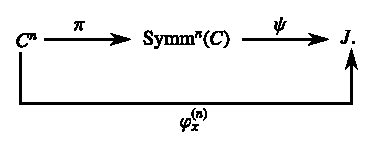
\includegraphics{chap6/fig12.eps}
\end{figure}
Passing to formal completions, we get a factorization
\begin{figure}[H]
\centering
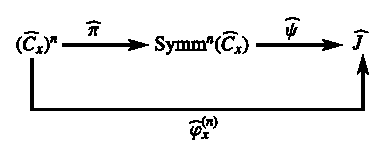
\includegraphics{chap6/fig13.eps}
\end{figure}

We will first show that $(\widehat{\psi})^{*}$ is injective on $H^{1}_{\DR}$, by showing that the map $\widehat{\psi}$ has a cross-section. This in turn follows from the global fact that $\psi$ is a $P^{n-g}$-bundle over $J$ which is locally trivial on $J$ for the Zariski topology. To see this last point, take a Poincare line bundle $\mathscr{C}$ on $C\times J$. Because $n\geq 2g-1$, the Riemann-Roch theorem and standard base-changing results show that the sheaf on $J$ given by $(\pr_{2})_{*}(\mathscr{C}\otimes\pr^{*}_{1}(I^{-1}(x)^{\otimes n}))$ is locally free of rank $n+1-g$. The associated projective bundle is naturally isomorphic to $\psi$.

It remains only to show that the kernel of the map
$$
(\widehat{\pi})^{*}:H^{1}_{\DR}(\Symm^{n}(\widehat{C}_{x})/R)\to H^{1}_{\DR}((\widehat{C}_{x})^{n}/R)
$$
is annihilated by $n!$. But if a one-form $\omega$ on $\Symm^{n}(\widehat{C}_{x})$ becomes exact when pulled back to $(\widehat{C}_{x})^{n}$, say $\omega=\df$ with $f\in A((\widehat{C}_{x})^{n})$, then 
$$
n!\omega=\sum\limits_{\sigma\in \mathfrak{S}_{n}}\sigma(\omega)=d\left(\sum\limits_{\sigma\in\mathfrak{S}_{n}}\sigma(f)\right)
$$
is exact on $\Symm^{n}(\widehat{C}_{x})$.
\end{proof}

\begin{remark*}
The fact that for $n$ large the symmetric product $\Symm^{n}(C)$ is a projective bundle over $J$ may be used to give a direct proof that $C$ and $J$ have isomorphic $H^{1}$'s in any of the usual theories (e.g., coherent, Hodge, De Rham, etale, crystalline...).
\end{remark*}

\medskip
\noindent
{\bf Theorem \thnum{5.9.5}.\label{art6-thm5.9.5}}~{\em Let $k$ be a perfect field of characteristic $p>0$, $\overline{k}$ its algebraic closure, $C$ a projective smooth curve over $W(k)$ with geometrically connected fibre, $J=\Pic^{0}(C/W(k))$ its jacobian, $x\in C(W(k))$ a rational\pageoriginale point of $C$, and $\varphi_{x}:C\to J$ the corresponding Albanese mapping. There is an exact sequence of $W$-modules}
\begin{figure}[H]
\centering
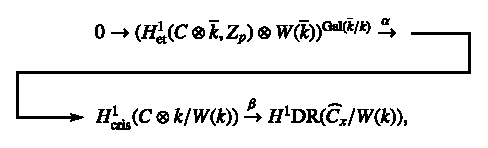
\includegraphics{chap6/fig14.eps}
\end{figure}
{\em the maps in which are functorial in $(C,x)\otimes k$ as pointed $k$-scheme}.

\begin{proof}
The map $\alpha$ is defined exactly as was its abelian variety analogue (cf. \ref{art6-thm5.7.1}); the map $\beta$ is defined as the composite
\begin{figure}[H]
\centering
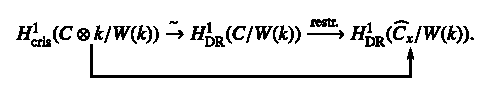
\includegraphics{chap6/fig15.eps}
\end{figure}
By construction, $\alpha$ is functorial in $(C,x)\otimes k$. By lemma (\ref{art6-lem5.8.2}), $\beta$ is similarly functorial. To see that the sequence is {\em exact}, use the fact that the Albanese map induces isomorphisms on both crystalline (or de Rham!) and etale $H^{1}$'s, (cf. SGAI, Exp. XI, last page, for the etale case), i.e., we have a commutative diagram
{\fontsize{8}{10}\selectfont
\[
\xymatrix@C=.55cm{
0\ar[r] & (H^{1}_{\et}(J\otimes \overline{k},Z_{p})\otimes W(\overline{k}))^{\Gal}\ar[d]_{\rotatebox{90}{$\sim$}}^{(\varphi,\otimes k)^{*}}\ar[r]^-{\alpha.} & H^{1}_{\cris}(J\otimes k/W(k)) \ar[d]_{\rotatebox{90}{$\sim$}}^{(\varphi,\otimes k)^{*}}\ar[r] & D(\widehat{J}/W(k))\ar@{_(->}[d]^{(\widehat{\varphi}_{x})^{*}}\ar[r] & 0\\
 & (H^{1}_{\et}(C\otimes \overline{k},Z_{p})\otimes W(\overline{k}))^{(\Gal(\overline{k}/k))}\ar[r]^-{\alpha} & H^{1}_{\cris}(C\otimes k/W(k))\ar[r]^-{\beta} & H^{1}_{\DR}(\widehat{C}_{x}/W(k)). & 
}
\]}\relax
\end{proof}

\medskip
\noindent
{\bf Corollary \thnum{5.9.6}.\label{art6-coro5.9.6}}~(1)~{\em The kernel of the ``formal expansion at a point'' map}
$$
H^{1}_{\DR}(C/W(k))\to H^{1}_{\DR}(\widehat{C}_{x}/W(k))
$$
{\em in $H^{1}_{\DR}(C/W(k))\simeq H^{1}_{\cris}(C\otimes k/W(k))$ is the ``slope-zero'' part of the $F$-crystal $H^{1}_{\cris}(C\otimes k/W(k))$, i.e., we have a commutative diagram}
{\fontsize{7}{9}\selectfont
\[
\xymatrix@C=.42cm{
0\ar[r] & (H^{1}_{\et}(C\otimes \overline{k},Z_{p})\otimes W(\overline{k}))\ar@{=}[d]\ar[r]^-{(\Gal(\overline{k}/k))} & H^{1}_{\DR}(C/W)\ar[r] & (\text{image of~}H^{1}_{\DR}(C/W)\text{~in~} H^{1}_{\DR}(\widehat{C}_{x}/W(k))\ar[r] & 0\\
0\ar[r] & (\text{slope~}0)\ar[r] & H^{1}_{\cris}(C\otimes k/W(k))\ar[u]^{\rotatebox{90}{$\sim$}}\ar[r] & (\text{slope}>0)\ar[u]^{\rotatebox{90}{$\sim$}}\ar[r] & 0.
}
\]}\relax
(2) {\em The image of the ``formal expansion at a point'' map is the ``slope $>0$'' quotient of $H^{1}_{\cris}(C\otimes k/W(k))$; this quotient is isomorphic, via the Albanese map $\varphi_{x}$, to $D(\widehat{J}/W(k))$.}

\bigskip
\noindent
{\bf VI. Applications\pageoriginale to congruences and to Honda's conjecture.} Let $C$ be a projective smooth curve over $W(F_{q})$ with geometrically connected fibres. Let $G$ be a finite group of order prime to $p$, all of whose absolutely irreducible complex representations are realizable over $W(F_{q})$ (e.g., if the exponent of $G$ divides $q-1$, this is automatic). Suppose that $G$ operates on $C$ by $W(F_{q})$-automorphisms. Then $G$ operates also on $C\otimes F_{q}$ by $F_{q}$-automorphisms. For each absolutely irreducible representation $\rho$ of $G$, let $P_{1,\rho}(T)\in W(F_{q})[T]$ be the numerator of the associated $L$-function $L(C\otimes F_{q}/F_{q},G,\rho;T)$;
$$
P_{1,\rho}(T)=1+a_{1}(\rho)T+\cdots+a_{r}(\rho)T^{r}.
$$ 

Let $\omega\in H^{0}(C,\Omega^{1}_{C/W})^{\rho}$ be a differential of the first kind on $C$ which lies in the $\rho$-isotypical component of $H^{0}(C,\Omega^{4}_{C/W})$. Let $x\in C(W(F_{q}))$ be a rational point on $C$, and let $X$ be a parameter at $x$ (i.e., $X$ is a coordinate for the one-dimensional pointed formal Lie variety $\widehat{C}_{x}$ over $W(F_{q})$). Consider the formal expansion of $\omega$ around $x$:
$$
\omega=\sum\limits_{n\geq 1}b(n)\cdot X^{n}\dfrac{dX}{X}\quad b(n)\in W(F_{q}).
$$
We extend the definition of $b(n)$ to rational numbers $n>0$ by decreeing that $b(n)=0$ unless $n$ is an integer.

\medskip
\noindent
{\bf Theorem \thnum{6.1}.\label{art6-thm6.1}}~{\em In the above situation, the coefficients $b(n)$ satisfy the congruences}
$$
\frac{b(n)}{n}+a_{1}(\rho)\cdot \frac{b(nq)}{nq}+\cdots+a_{r}(\rho)\frac{b(nq^{r})}{nq^{r}}\in pW(F_{q})
$$
{\em for every rational $n>0$.}

\begin{proof}
Let $J$ denote the Jacobian of $C/W(F_{q})$, and denote by $\widehat{\omega}\in \underline{\omega}_{J}$ the unique invariant one-form on $J$ which pulls back to give $\omega$ under the Albanese mapping $\varphi_{x}$. The group $G$ operates, by functoriality, on $J$ and on $\underline{\omega}_{J}$, and the isomorphism $\underline{\omega}_{J}\xrightarrow{\sim}H^{0}(C,\Omega^{1}_{C/W})$ is $G$-equivariant. Therefore $\widetilde{\omega}$ lies in $(\underline{\omega}_{J})^{\rho}$. Via the $G$-equivariant inclusion
$$
\underline{\omega}_{J}\subset D_{(p)}(\widehat{J}/W)
$$
we\pageoriginale have
$$
\widetilde{\omega}\in (D_{(p)}(\widehat{J}/W))^{\rho}
$$

Now let $F$ denote the Frobenius endomorphism of $J\otimes F_{q}$ relative to $F_{q}$. Then both $F$ and the group $G$ act on $J\otimes F_{q}$. By \eqref{art6-prop4.2}, we know that
$$
(F^{r}+a_{1}(\rho)F^{r-1}+\cdots+a_{r}(\rho))\cdot \Proj(\rho)=0
$$
in $\foprod{\End(J\otimes F_{q})}{W(F_{q})}{Z}$. Because $D(\widehat{J}/W)$ is an additive functor of $J\otimes F_{q}$ with values in $W(F_{q})$-modules, and $\widetilde{\omega}$ lies in its $\rho$-isotypical component, it follows that
\begin{equation*}
F^{r}(\widetilde{\omega})+a_{1}(\rho)F^{r-1}(\widetilde{\omega})+\cdots+a_{r}(\rho)\cdot \widetilde{\omega}=0\tag{6.1.1}\label{art6-eq6.1.1}
\end{equation*}
in $D_{(p)}(\widehat{J}/W)$.

The Albanese map $\varphi_{x}:C\to J$ induces a map
$$
\widehat{\varphi}_{x}:\widehat{C}_{x}\to \widehat{J},
$$
whence a map
$$
D_{(p)}(\widehat{J}/W)\subset H^{1}_{\DR}(\widehat{J}/W;(p))\xrightarrow{(\widehat{\varphi}_{x})^{*}}H^{1}_{\DR}(\widehat{C}_{x};(p))
$$
which is functorial in the pointed schemes $(\widehat{J},0)\otimes F_{q}$ and $(\widehat{C}_{x},x)\otimes F_{q}$. So if we denote also by $F$ the $q$-th power Frobenius endomorphism of $\widehat{C}_{x}\otimes F_{q}$, we have
$$
(\widehat{\varphi}_{x})^{*}\circ F=F\circ (\widehat{\varphi}_{x})^{*},
$$
whence a relation
\begin{equation*}
F^{r}(\omega)+a_{1}(\rho)F^{r-1}(\omega)+\cdots+a_{r}(\rho)\cdot \omega=0\tag{6.1.2}\label{art6-eq6.1.2}
\end{equation*}
in $H^{1}_{\DR}(\widehat{C}_{x}/W;(p))$.

The asserted congruences on the $b(n)$'s are simply the spelling out of this relation. Explicitly, in terms of the chosen coordinate $X$ for $\widehat{C}_{x}$, a particularly convenient pointed lifting of $F$ on $\widehat{C}_{x}\otimes F_{q}$ is provided by
$$
F:X\mapsto X^{q}.
$$

In\pageoriginale terms of the isomorphism
$$
H^{1}_{\DR}(\widehat{C}_{x}/W;(p))\xleftarrow{\sim}\frac{\{f\in K[[X]]|f(0)=0,\df\text{~integral}\}}{\{f\in pW[[X]]|f(0)=0\}}
$$
the cohomology class of $\omega$ is represented by the series
$$
f(X)=\sum\limits_{n>0}\frac{b(n)}{n}X^{n},
$$
and the cohomology class of $F^{i}(\omega)$ is represented by
$$
f(X^{q^{i}})=\sum \frac{b(n)}{n}X^{nq^{i}}.
$$
The relation \eqref{art6-eq6.1.3} thus asserts that
$$
f(X^{q^{r}})+a_{1}(\rho)f(X^{q^{r-1}})+\cdots+a_{r}(\rho)f(X)
$$
is a series whose coefficients all lie in $pW(F_{q})$. The congruence asserted in the statement of the theorem is precisely that the coefficient of $X^{nq^{r}}$ in this series lies in $pW(F_{q})$.
\end{proof}

\begin{remark*}
In the special case $G=\{e\}$, $\rho$ trivial, the polynomial $P_{1,\rho}(T)$ is the numerator of the zeta function of $C\otimes F_{q}$, and every differential of the first kind $\omega\in H^{i}(C,\Omega^{1}_{C/W})$ is $\rho$-isotypical. The resulting congruences on the coefficients of differentials of the first kind were discovered independently by Cartier and by Honda in the case of elliptic curves, and seem by now to be ``well-known'' for curves of any genus. (\cite{art6-key1}, \cite{art6-key5}, \cite{art6-key8}, \cite{art6-key22}).
\end{remark*}

\noindent
{\bf Theorem \thnum{6.2}.\label{art6-thm6.2}}~{\em Hypothesis and notation as above, suppose that the polynomial $P_{1,\rho}(T)$ is linear}
$$
P_{1,\rho}(T)=1+a_{1}(\rho)T,
$$
{\em i.e., that $\rho$ occurs in $H^{1}$ with multiplicity one. Then}
\begin{itemize}
\item[(1)] {\em $a_{1}(\rho)$ is equal to the exponential sum $S(C\otimes F_{q}/F_{q},\rho,1)$ and for every $n\geq 1$ we have}
$$
(-a_{1}(\rho))^{n}=-S(C\otimes F_{q}/F_{q},\rho,n).
$$

\item[(2)] {\em If\pageoriginale $\rho$ occurs in $H^{0}(C,\Omega^{1}_{C/W})$, then $\ord_{p}(a_{1}(\rho))>0$, i.e., $a_{1}(\rho)$ is not a unit in $W(F_{q})$.}

\item[(3)] {\em If $\rho$ occurs in $H^{0}(C,\Omega^{1}_{C/W})$, choose $\omega\in H^{0}(C,\Omega^{1}_{C/W})^{\rho}$ to be non-zero, and such that at least one of coefficients $b(n)$ is a unit in $W(F_{q})$. For any $n$ such that $b(n)$ is a unit, the coefficients $b(nq)$, $b(nq^{2}),\ldots$ are all non-zero, and we have the limit formulas (in which $\overline{\rho}$ denotes the contragradient representation)}
\begin{align*}
-S(C\otimes F_{q}/F_{q},\rho,1) &= -a_{1}(\rho)=\lim\limits_{N\to \infty} \frac{q\cdot b(nq^{N})}{b(nq^{N+1})}\\[3pt]
-S(C\otimes F_{q}/F_{q},\overline{\rho},1) &= -a_{1}(\overline{\rho})=\frac{-q}{a_{1}(\rho)}=\lim\limits_{N\to \infty}\frac{b(nq^{N+1})}{b(nq^{N})}.
\end{align*}
\end{itemize}

\begin{proof}
If $\rho$ occurs in $H^{1}$ with multiplicity {\em one}, then $\rho$ must be a non-trivial representation of $G$ (for if $\rho$ were the trivial representation, $G$ would have a one-dimensional space of invariants in $H^{1}$; but the space of invariants in $H^{1}$ of the quotient curve $C\otimes F_{q}$ modulo $G$, so is {\em even-dimensional}!). Therefore $\rho$ does {\em not} occurs in $H^{0}$ or $H^{2}$, as both of these are the trivial representation of $G$. The first assertion now results from \eqref{art6-lem1.1}.

If $\rho$ also occurs in $H^{0}(C,\Omega^{1}_{C/W})$, pick any non-zero $\omega$ in 
$$
H^{0}(C,\Omega^{1}_{C/W})^{\rho}
$$ 
and look at its formal expansion around $x$:
$$
\omega=\sum b(n)X^{n}\dfrac{dX}{X}.
$$
An elementary ``$q$-expansion principle''-argument (cf. \cite{art6-key28}) shows that if all $b(n)$ are divisible by $p$, then $\omega$ is itself divisible by $p$ in $H^{0}(C,\Omega^{1}_{C/W})$. So after dividing $\omega$ by the highest power of $p$ which divides all $b(n)$, we obtain an element $\omega\in H^{0}(C,\Omega^{1}_{C/W})^{\rho}$ which has some coefficient a unit.

Consider the congruences satisfied by the $b(n)$:
$$
\frac{b(n)}{n}+a_{1}(\rho)\frac{b(nq)}{nq}\in pW(F_{q}).
$$
If\pageoriginale $a_{1}(\rho)$ were a {\em unit}, we could infer (by induction on the precise power of $p$ dividing $n$) that
$$
\text{for {\em all} } n\geq 1, \ \frac{q}{p}\cdot \frac{b(n)}{n}\in W(F_{q}).
$$

In particular, we would find that $\dfrac{q}{p}\cdot \omega$ is {\em formally} exact at $x$, which by \eqref{art6-coro5.9.3} is impossible.

Given that $a_{1}(\rho)$ is a non-unit, choose $n$ such that $b(n)$ {\em is} a unit. Then
$$
\ord (b(n)/n)\leq 0.
$$
From the congruences
\begin{align*}
\frac{b(n)}{n} &\equiv -a_{1}(\rho)\frac{b(nq)}{nq}\quad \mod pW\\
\vdots\quad & \\
\frac{b(nq^{N})}{nq^{N}} &\equiv -a_{1}(\rho)\frac{b(nq^{N+1})}{nq^{N+1}} \ \mod pW
\end{align*}
and the fact that $\ord(a_{1}(\rho))>0$, it follows easily by induction on $N$ that
$$
\ord\left(\frac{b(nq^{N})}{nq^{N}}\right)=\ord(b(n)/n)-N\ord (a_{1}(\rho)).
$$
Therefore we may {\em divide} the congruences, and obtain 
\begin{align*}
& \ord\left(\frac{qb(nq^{N})}{b(nq^{N+1})}+a_{1}(\rho)\right)\geq 1+(N+1)\ord(a_{1}(\rho))-\ord(b(n)/n)\\[3pt]
& \ord\left(\frac{b(nq^{N+1})}{b(nq^{N})}+\frac{q}{a_{1}(\rho)}\right)\geq 1+\ord\left(\frac{q}{a_{1}(\rho)}\right)+N\ord(a_{1}(\rho))-\ord\left(\frac{b(n)}{n}\right).
\end{align*}
Letting $N\to \infty$, we get the asserted limit formulas for $-a$, $(\rho)$ and for $-q/a_{1}(\rho)$. By the Riemann Hypothesis for curves over finite fields, we know that $-q/a_{1}(\rho)$ is the complex conjugate $\overline{a_{1}(\rho)}$. Let $\overline{\rho}$ denote the contragradient representation of $\rho$; because the definition of the $L$-series $L(C\otimes F_{q}/F_{q},G,\rho;T)$ is purely algebraic, the $L$-series for $\overline{\rho}$ is obtained by applying (any) complex conjugation to the coefficients of the $L$-series for\pageoriginale $\rho$. Therefore $\overline{a_{1}(\rho)}=a_{1}(\overline{\rho})$, and $\overline{\rho}$ also occurs in $H^{1}$ with multiplicity one.
\end{proof}

\smallskip
\noindent
{\bf Example \thnum{6.3}.\label{art6-exam6.3}}~Consider the Fermat curve of degree $N$ over $W(F_{q})$, with $q\equiv 1\mod N$. For each integer $0\leq r\leq N-1$, denote by $\chi_{r}$ the character of $\mu_{N}$ given by
$$
\chi_{r}(\zeta)=\zeta^{r}.
$$
We know that under the action of $\mu_{N}\times \mu_{N}$ (acting as $(x,y)\to (\zeta x,\zeta' y)$ in the affine model $x^{N}+y^{N}=1$), the characters which occurs in $H^{1}$ are precisely
$$
\chi_{r}\times \chi_{s}\qquad 1\leq r, s\leq N-1, r+s\neq N,
$$
each with multiplicity one. Those which occur in $H^{0}(\Omega^{1})$ are precisely the
$$
\chi_{r}\times \chi_{s}\qquad 1\leq r,s\leq N-1, r+s<N,
$$
the corresponding eigen-differential $\omega_{r,s}$ is given by
$$
\omega_{r,s}=x^{r}y^{s}\frac{dx}{xy^{N}}.
$$
If we expand $\omega_{r,s}$ at the point $(x=0,y=1)$, in the parameter $x$, we obtain 
\begin{align*}
\omega_{r,s} &= x^{r}(1-x^{N})\frac{s}{N}-1\cdot \frac{dx}{x}\\[3pt]
&= \sum\limits_{j\geq 0}(-1)^{j}\left(\frac{s}{N}{\displaystyle{\mathop{-}\limits_{j}}}1\right)x^{r+Nj}\frac{dx}{x}\\[3pt]
&= \sum\limits_{n\geq 1}b(n)x^{n}\dfrac{dx}{x}.
\end{align*}
Conveniently, the first non-vanishing coefficient $b(r)$ is $1$. The successive coefficients $b(rq^{n})$ are given by
$$
b(rq^{n})=(-1)^{\frac{r}{N}(q^{n}-1)}\cdot 
\left(\begin{matrix} 
\frac{s}{N}-1\\[4pt]
\frac{r}{N}(q^{n}-1)
\end{matrix}
\right).
$$
The\pageoriginale eigenvalue of $F$ on the $\chi_{r}\times \chi_{s}$-isotypical component of $H^{1}$ is the {\em negative} of the Jacobi sum $J_{q}(\chi_{r},\chi_{s})$. There we obtain the limit formulas
\begin{align*}
-J_{q}(\chi_{r},\chi_{s}) &= \lim\limits_{n\to \infty}
\frac{
(-1)^{\frac{r}{N}(q-1)\cdot q^{n}}
\left(\begin{matrix}
\frac{s}{N}-1\\[4pt]
\frac{r}{N}(q^{n}-1)
\end{matrix}\right)}
{\left(\begin{matrix}
\frac{s}{N}-1\\[4pt]
\frac{r}{N}(q^{n+1}-1)
\end{matrix}\right)}\\[10pt]
-J_{q}(\chi_{N-r},\chi_{N-s}) &= 
\lim\limits_{n\to \infty}
\frac{(-1)^{\frac{r}{N}(q-1)\cdot q^{n}}\cdot 
\left(
\begin{matrix}
\frac{s}{N}-1\\[4pt]
\frac{r}{N}(q^{n+1}-1)
\end{matrix}
\right)}{
\left(
\begin{matrix}
\frac{s}{N}-1\\[4pt]
\frac{r}{N}(q^{n}-1)
\end{matrix}
\right)}
\end{align*}
valid for $1\leq r$, $s\leq N-1$, $r+s\neq N$. These formulas are the ones originally conjectured by Honda, and recently interpreted by Gross-Koblitz \cite{art6-key14} in terms of Morita's $p$-adic gamma function.

\bigskip
\noindent
{\bf VII. Application of Gauss sums.} In this chapter we will analyze the cohomology of certain Artin-Schreier curves, and then obtain a limit formula for Gauss sums in the style of the preceding section.

We fix a prime $p$, an integer $N\geq 2$ prime to $p$, and consider the smooth affine curve $U$ over $Z[1/N(p-1)]$ defined by the equation
$$
T^{p}-T=X^{N}.
$$
It may be compactified to a projective smooth curve $C$ over $Z[1/N(p-1)]$ with geometrically connected fibres by adding a single ``point at infinity'', along which $T^{-1/N}$ is a uniformizing parameter.

The group-scheme $\mu_{N(p-1)}$ operates on $U$, by
$$
\zeta :(T,X)\to (\zeta^{N}T,\zeta X).
$$
This\pageoriginale action extends to $C$, and fixes the point at infinity.

A straightforward computation gives the following lemma.

\medskip
\noindent
{\bf Lemma \thnum{7.1}.\label{art6-lem7.1}}~(1)~{\em The genus of $C$ is $\frac{1}{2}(N-1)(p-1)$, and a basis of everywhere holomorphic differentials on $C$ is given by the forms}
$$
X^{a}T^{b}\frac{dT}{X^{N-1}}
$$
{\em with $0\leq a\leq N-2$, $0\leq b\leq p-2$, and $pa+Nb<(p-1)(N-1)-1$.}
\begin{itemize}
\item[(2)] {\em The space $H^{1}_{\DR}(C\otimes Q/Q)\xrightarrow{\sim} H^{1}_{\DR}(U\otimes Q/Q)$ has dimension $(N-1)(p-1)$, any $d$ basis is given by the cohomology classes of the forms}
$$
X^{q}T^{b}\frac{dT}{X^{N-1}}\qquad 0\leq a\leq N-2, \ 0\leq b\leq p-2.
$$

\item[(3)] {\em The characters of $\mu_{N(p-1)}$ which occur in $H^{1}_{\DR}(C\otimes Q/Q)$ are precisely those whose restrictions to $\mu_{N}$ is non-trivial, and each of these occurs with multiplicity one.}
\end{itemize}

In characteristic $p$, there are new automorphisms. The additive group $F_{p}$ operates on $C\otimes F_{p}$ by
$$
a:(T,X)\to (T+a,X).
$$
This action does not commute with the action of $\mu_{N(p-1)}$. However, the two together define an action of the semi-direct product
$$
F_{p} \ltimes \mu_{N(p-1)}
$$
formed via the homomorphism
$$
\mu_{N(p-1)}\xrightarrow{-N} \mu_{p-1}\simeq F^{\times}_{p}=\Aut (F_{p})
$$
Explicitly, the multiplication is
$$
(a,\zeta)(b,\zeta_{1})=(a+\zeta^{-N}b,\zeta\zeta_{1}),
$$
and the action is
$$
(a,\zeta):(T,X)\to (\zeta^{N}T+\zeta^{N}a,\zeta X).
$$

The\pageoriginale group $F_{p}\ltimes \mu_{N(p-1)}$ contains $F_{p}\times \mu_{N}$ as a normal subgroup, acting on $C\otimes F_{p}$ in the usual manner.

\begin{remark*}
This action of a group of order $p(p-1)N$ on a curve of genus $g=\frac{1}{2}(p-1)(N-1)$ provides a nice example of how ``wrong'' the characteristic zero estimate $84(g-1)$ can become in the presence of wild ramification!
\end{remark*}

Let $E$ be a number field containing the $N(p-1)$'st roots of unity, $\sfP$ a $p$-adic place of $E$, $F_{q}$ a finite extension of the residue field $F_{N(\sfP)}$, of $\sfP$, $G$ the abstract group $F_{p}\ltimes \mu_{N(p-1)}(F_{q})$. Let $H^{1}$ denote any of the vector spaces $\foprod{H^{1}_{l}(C\otimes F_{q})}{E_{\lambda}}{Z_{l}}$ for $l\neq p$, or $H^{1}_{\cris}(C\otimes F_{q}/W(F_{q}))\otimes K$. 

By functoriality, the group $G$ operates on $H^{1}$. Because the center of $G$ is $\mu_{N}(F_{q})$, the decomposition
$$
H^{1}=\otimes (H^{1})^{\chi}
$$
of $H^{1}$ according to the characters of $\mu_{N}$ is $G$-stable.

\medskip
\noindent
{\bf Proposition \thnum{7.2}.\label{art6-prop7.2}}~{\em For each of the $N-1$ non-trivial $E$-valued characters $\chi$ of $\mu_{N}(E)\xrightarrow{\sim}\mu_{N}(F_{N(\sfP)})=\mu_{N}(F_{q})$, the corresponding eigenspace $(H^{1})^{\chi}$ is a $p-1$ dimensional absolutely irreducible representation of $G$; the restriction to $F_{p}$ of $(H^{1})^{\chi}$ is the augmentation representation of $F_{p}$; the restriction to $\mu_{N(p-1)}(F_{q})$ of $(H^{1})^{\chi}$ is the induction, from $\mu_{N}$ to $\mu_{N(p-1)}$, of $\chi$.}

\begin{proof}
All assertions except for the $G$-irreducibility of $(H^{1})^{\chi}$ follow immediately from the preceding lemma, giving the action of $\mu_{N(p-1)}$, and from Corollary \eqref{art6-coro2.2}, giving the action of $F_{p}\times \mu_{N}$. The irreducibility follows from these facts together with the fact that in {\em any} complex representation of $G$, the set of characters of $F_{p}$ which occur is stable under the action of $\mu_{N(p-1)}$ in $F_{p}$ by conjugation; because this action has only the two orbits $F^{\times}_{p}$ and $0$, as soon as any one non-trivial character of $F_{p}$ occurs, {\em all} non-trivial characters must also occur.
\end{proof}

\noindent
{\bf Corollary \thnum{7.3}.\label{art6-coro7.3}}~(1)~{\em Over any finite extension $F_{q}$ of $F_{p}$ which contains all the $N(p-1)$'st roots of unity (i.e., $q\equiv 1\mod N(p-1)$), the Frobenius $F$ relative to $F_{q}$ operates as a scalar on each of the spaces $(H^{1})^{\chi}$, $\chi$ a non-trivial character of $\mu_{N}$. This scalar is the common value}
$$
-g_{q}(\psi,\chi;\sfP)
$$
{\em of\pageoriginale the Gauss sums attached to any of the non-trivial additive characters $\psi$ of $F_{\sfP}$.}

\begin{proof}
Over such an $F_{q}$, Frobenius commutes with the action of $G$ on $H^{1}$, so it acts on each $(H^{1})^{\chi}$ as a $G$-morphism. Because $(H^{1})^{\chi}$ is $G$-irreducible, this $G$-morphism must be a scalar, and this scalar is equal to {\em any} eigenvalue of $F$ on $(H^{1})^{\chi}$. As we have already seen \eqref{art6-lem2.1}, these eigenvalues are precisely the asserted Gauss sums, corresponding to the decomposition of $(H^{1})^{\chi}$ under $F_{p}$.
\end{proof}

The common value of these Gauss sums over a sufficiently large $F_{q}$ is itself a Jacobi sum, in consequence of the fact that universally, i.e., over $Z[1/N(p-1)]$, the curve $C$ is the {\em quotient} of the Fermat curve Fermat $(N(p-1))$ of degree $N(p-1)$ by the {\em subgroup} $H$ of $\mu_{N(p-1)}\times \mu_{N(p-1)}$ consisting of all $(\zeta_{1},\eta_{2})$ satisfying
$$
\zeta^{p-1}_{1}=\zeta^{p}_{2}
$$
Explicitly, the map is given rationally by the formulas
\begin{align*}
& (W,V)\text{~ on~ } W^{N(p-1)}+V^{N(p-1)}=1\\
&\quad \downarrow\\
&(T,X)\text{~ on~ }T^{p}-T=X^{N}\\
& T=1/V^{N}, X=W^{p-1}/V^{p}.
\end{align*}

\noindent
{\bf Lemma \thnum{7.4}.\label{art6-lem7.4}}~{\em Let $\chi_{1}$ be a character of $\mu_{N(p-1)}$ whose restriction to $\mu_{N}$ is non-trivial. Under the map}
$$
H^{1}_{\DR}(C\otimes Q/Q)\xrightarrow{\sim} H^{1}(\text{Fermar~}(N(p-1))\otimes Q/Q)^{H}
$$
{\em we have}
$$
H^{1}_{\DR}(C\otimes Q/Q)^{\chi_{1}}\xrightarrow{\sim} H^{1}_{\DR}(\text{Fermat~}(N(p-1))\otimes Q/Q)^{\chi^{p-1}_{1}\times \chi^{-p}_{1}}
$$

\begin{proof}
That $H^{1}(C)\xrightarrow{\sim}H^{1}(\Fermat)^{H}$ in rational cohomology results from the Hochschild-Serre spectral sequence. Since the characters of $\mu_{N(p-1)}$ (resp of $\mu_{N(p-1)}\times \mu_{N(p-1)}$) occur, if at all, with multiplicity one in $H^{1}(C)$ (resp $H^{1}$ (Fermar)), it suffices to check that the $\chi_{1}$-eigenspace of $H^{1}(C)$ is mapped to the $(\chi^{p-1}_{1},\chi^{-p}_{1})$-eigenspace of $H^{1}$(Fermat). This we\pageoriginale do by inspection:
\begin{align*}
& X^{a}T^{b}\dfrac{dT}{X^{N-1}} =\\[3pt]
& \qquad = X^{a+1-N}T^{b+1}\frac{dT}{T}\mapsto \left(\frac{W^{p-1}}{V^{p}}\right)^{a+1-N}\left(Z^{-N}\right)^{b+1}\left(\frac{-NdZ}{Z}\right).
\end{align*}
\end{proof}

\noindent
{\bf Corollary \thnum{7.5}.\label{art6-coro7.5}}~{\em If $F_{q}$ contains the $N(p-1)$'st roots of unity, then for any non-trivial character $\chi$ of $\mu_{N}$, and extension $\chi_{1}$ of $\chi$ to $\mu_{N(p-1)}$ and any non-trivial additive character $\psi$ of $F_{p}$, the scalar by which $F$ acts on $H^{1}(C\otimes F_{q})^{\chi}$ is given by}
$$
\begin{cases}
F|H^{1}(C\otimes F_{q})^{\chi}=F|H^{1}(C\otimes F_{q})^{\psi\times \chi}=-g_{q}(\psi,\chi;\sfP)\\[3pt]
\qquad \Big|\Big|\\[3pt]
F|H^{1}(C\otimes F_{q})^{\chi_{1}}=F|H^{1}(\Fermat\otimes F_{q})^{\chi^{p-1}_{1}\times \chi^{-p}_{1}}=-J_{q}(\chi^{p-1}_{1},\chi^{-p}_{1};\sfP)
\end{cases}
$$

We now turn to the ``determination'' of the Gauss sum $-g_{q}(\psi,\chi;\sfP)$ over an $F_{q}$ which is merely required to contain the $N$'th roots of unity. Unless $p-1$ and $N$ are relatively prime, such an $F_{q}$ need {\em not} contain the $N(p-1)$'st roots of unity! Moreover, the Gauss sum does {\em not} in general lie in the Witt vectors $W(F_{q})$, as it does when $F_{q}$ contains the $N(p-1)$'st roots of unity!

Let $\pi$ denote any solution of
$$
\pi^{p-1}=-p.
$$
We recall without proof the following standard lemma (cf. \cite{art6-key31} or \cite{art6-key32}).

\medskip
\noindent
{\bf Lemma \thnum{7.6}.\label{art6-lem7.6}}~{\em The fields $Q_{p}(\zeta_{p})$ and $Q_{p}(\pi)$ coincide. There is a bijective correspondence}
$$
\text{\em primitive $p$'th roots of 1} \longleftrightarrow \text{\em solutions $\pi$ of $\pi^{p-1}=-p$}
$$
{\em under which $\zeta\longleftrightarrow \pi$ if and only if}
$$
\zeta\equiv 1+\pi \mod \pi^{2}.
$$

For each solution $\pi$ of $\pi^{p-1}=-p$, we denote by
$$
\psi_{\pi}:F_{p}\to Q_{p}(\zeta_{p})^{\times}
$$
the\pageoriginale unique non-trivial additive character which satisfies
$$
\psi_{\pi}(1)\equiv 1+\pi \mod \pi^{2}.
$$
If we fix a $W(F_{q})$-valued point $x$ on $C$, we have the map ``formal expansion at $x$''
$$
H^{1}_{\cris}(C\otimes F_{q}/W(F_{q}))\to H^{1}_{\DR}(\widehat{C}_{x}\otimes W(F_{q})/W(F_{q})).
$$
If we denote by $R$ the ring
$$
R=W(F_{q})[\pi]
$$
which is a free $W$-module of finite rank $(p-1)$, we may tensor with $R$ to obtain 
\[
\xymatrix{
H^{1}_{\cris}(C\otimes F_{q}/W(F_{q})){\displaystyle{\mathop{\otimes}\limits_{W}}} R\ar@{-}[d]^{\rotatebox{90}{$\backsim$}}\ar[rr] & & H^{1}_{\DR}(\widehat{C}_{x}\otimes R/R).\\
  H^{1}_{\DR}(C\otimes R/R)\ar[urr] & 
}
\]

\noindent
{\bf Theorem \thnum{7.7}.\label{art6-thm7.7}}~(1)~{\em For any $W(F_{q})$-valued point $x$ on $C$, the ``formal expansion'' map is injective :}
$$
H^{1}_{\cris}(C\otimes F_{q}/W(F_{q}))\hookrightarrow H^{1}_{\DR}(\widehat{C}_{x}\otimes W(F_{q})/W(F_{q}))
$$
\begin{itemize}
\item[(2)] {\em Let $\pi$ be any solution of $\pi^{p-1}=-p$, $\psi_{\pi}$ the corresponding additive character, $a$ an integer $1\leq a\leq N-1$ and $\chi_{a}$ the corresponding nontrivial character of $\mu_{N}(\chi_{a}(\zeta)=\zeta^{a})$. If we take for $x$ the point $(T=0,X=0)$ on $C$, with parameter $X$, then the image of}
$$
(H^{1}_{\cris}(C\otimes F_{q}/W(F_{q}))\otimes Q_{p}(\pi))^{\psi_{w}\times \chi_{a}}\to \foprod{H^{1}_{\DR}(\widehat{C}_{x}\otimes R/R)}{Q_{p}(\pi)}{R}
$$ 
{\em is the one-dimensional $Q_{p}(\pi)$-space spanned by the cohomology class of}
$$
\exp(-\pi X^{N})X^{a}\frac{dX}{X}=\sum b(n)X^{n}\frac{dX}{X}.
$$
\end{itemize}

\noindent
{\bf Corollary \thnum{7.8}.\label{art6-coro7.8}}~{\em Notations as above, let $f(X)$ denote the power series}
$$
f(X)=\sum\limits_{n\geq 1}b(n)\frac{X^{n}}{n}=\sum\limits_{n\geq 0}\frac{(-\pi)^{n}}{n!}\frac{X^{nN+a}}{nN+a}
$$
{\em Then\pageoriginale the series}
$$
f(X^{q})+g_{q}(\psi_{\pi},\chi_{a};\sfP)\cdot f(X)
$$
{\em has coefficients with bounded denominators, and we have a limit formula}
\begin{equation*}
\begin{cases}
-g_{q}(\psi_{\pi},\chi_{a};\sfP)=\lim\limits_{r\to \infty}\frac{q\cdot b(aq^{r})}{b(aq^{r+1})}\\[4pt]
\text{with}\quad b(aq^{r})=\frac{(-\pi)^{(q^{r}-1)\frac{a}{N}}}{((q^{r}-1)\frac{a}{N})!}
\end{cases}\tag{7.8.1}\label{art6-eq7.8.1}
\end{equation*}

We first deduce the corollary from the theorem. We know that $F$ has eigenvalue $-g_{q}(\psi_{\pi},\chi_{a};\sfP)$ on the $\psi_{\pi}\times \chi_{a}$-eigenspace of $H^{1}_{\cris}\otimes Q_{p}(\pi)$, hence $F$ has the same eigenvalue on the image of this one-dimensional eigenspace in $H^{1}_{\DR}(\widehat{C}_{x}\otimes R/R)\otimes Q_{p}(\pi)$. This image is spanned by the cohomology class of $\df$ : therefore $F+g_{q}(\psi_{\pi},\chi_{a};\sfp)$ annihilates the class of df mod torsion, whence
$$
f(X^{q})+g_{q}(\psi_{\pi},\chi_{a};\sfP)\cdot f(X)
$$
has bounded denominators. The final limit formula comes from looking successively at the coefficients of $X^{aq^{r+1}}$ in the above expression; one has
$$
\ord\left(\frac{b(aq^{r})}{aq^{r}}+g_{q}(\psi_{\pi},\chi_{a};\sfp)\cdot \frac{b(aq^{r+1})}{aq^{r+1}}\right)\geq -A
$$
for some constant $A$ independent of $r$. An explicit elementary calculation shows that
$$
\ord \left(\frac{b(aq^{r})}{aq^{r}}\right)\to -\infty\quad\text{as}\quad r\to +\infty,
$$
and this allows us to ``divide'' the additive congruence and obtain the asserted limit formula.

It remains to prove the theorem. In view of the exact sequence of \eqref{art6-thm5.9.5}, the injectivity of
$$
H^{1}_{\cris}(C\otimes F_{q}/W(F_{q}))\to H^{1}_{\DR}(\widehat{C}_{x}\otimes W/W)
$$
is\pageoriginale equivalent to the {\em absence} of any $p$-adic unit eigenvalues of $F$ in $H^{1}_{\cris}$. But these eigenvalues are the Gauss sums
$$
-g_{q}(\psi,\chi)\equiv -\sum \psi_{q}(x)\chi_{q}(x).
$$
Because $\psi_{q}(x)\equiv 1(\pi)$ for all $x$, while $\chi_{q}$ is a {\em non-trivial} character of $F^{x}_{q}$, we have
$$
-g(\psi,\chi)\equiv -\sum \chi_{q}(x)=0\mod \pi.
$$
(Alternately, one could observe that each non-trivial character $\chi$ of $\mu_{N}$ has at least one extension $\chi_{1}$ to $\mu_{N(p-1)}$ which occurs in $H^{0}(C\otimes Q,\Omega^{1}_{C\otimes Q})$; the eigenvalue of $F^{p-1}$ on this eigenspace is then a non-unit by \eqref{art6-eq6.2.2}; as $F^{p-1}$ is a scalar on $(H^{1})^{\chi}$, this scalar is non-unit.)

It remains to verify that the image of the $\psi_{\pi}\times \chi_{a}$-eigenspace is indeed spanned by
$$
\exp(-\pi X^{N})X^{a}\frac{dX}{X}
$$
This seems to require the full strength of the Washnitzer-Monsky ``dagger'' cohomology, as follows. Let $A^{t}$ denote the ``weak completion'' of the coordinate ring $R[T,X]/(T^{p}-T-X^{N})$ of $U\otimes R$. Because $U\otimes F_{q}$ is a ``special affine variety'' with coordinate $X$, there are {\em unique} liftings to $A^{t}$ of the actions of $F$ and of the group $F_{p}\otimes \mu_{N}$ whose effect on $X$ is given by
$$
\left\{
\begin{aligned}
F(X) &= X^{q}\\
(a,\zeta)(X) &= \zeta X.
\end{aligned}
\right.
$$
Thanks to Dwork, we know that the power series in $T$
$$
\exp (\pi T-\pi T^{p})
$$
actually lies in $R[T]^{t}$, and hence in $A^{t}$ for any $\pi$ satisfying $\pi^{p-1}=-p$. As Monsky pointed out, under the action of $F_{p}$ and $A^{t}$, this series transforms by the character $\psi_{\pi}$. It follows that for $1\leq a\leq N-1$ the differential form
$$
\exp (\pi T-\pi T^{p})X^{a}\frac{dX}{X}
$$
transforms\pageoriginale by $\psi_{\pi}\times \chi_{a}$ under the action of $F_{p}\times \mu_{N}$. Therefore its cohomology class in
$$
H^{1}_{W-M}(U\otimes F_{q};R)\otimes Q{\displaystyle{\mathop{=}\limits^{\text{dfn}}}}H^{1}(\Omega^{\bigdot}_{U\otimes R/R}\otimes A^{t})\otimes Q
$$
lies in the $\psi_{\pi}\times \chi_{a}$ eigenspace of $H^{1}_{W-M}$. A direct computation (\cite{art6-key31}, \cite{art6-key32}) shows that each of these eigenspaces is one-dimensional, and is spanned by the above-specified form.

Furthermore, there is a natural ``formal expansion map'' attached to any $R$-valued point $x$ of $U$;
$$
H^{1}_{W-M}(U\otimes F_{q};R)\to H^{1}_{\DR}(\widehat{U}_{x}\otimes R/R).
$$
For the particular choice of point $(T=0,X=0)$, the formal expansion map carries
$$
\exp (\pi T-\pi T^{p})X^{a}\frac{dX}{X}\mapsto \exp (-\pi X^{N})X^{a}\dfrac{dX}{X}.
$$

To conclude the proof, we need to {\em identify} $H^{1}_{WM}(U\otimes F_{q};R)\otimes Q$ with $H^{1}_{\cris}(C\otimes F_{q}/R)\otimes Q$ in a way compatible with the formal expansion map and with the action of $F$ and of $F_{p}\times \mu_{N}$. We will do this with a somewhat ad hoc argument.

Because $U$ is the complement of a single point in $C$, it follows from the theory of residues for both $H_{\DR}$ and $H_{W-M}$ that we have isomorphisms
$$
H^{1}_{\DR}(C\otimes R/R)\otimes Q\xrightarrow{\sim}H^{1}_{\DR}(U\otimes R/R)\otimes Q\xrightarrow{\sim}H^{1}_{W-M}(U\otimes F_{q};R)\otimes Q.
$$
These sit in a commutative diagram
\begin{figure}[H]
\centering
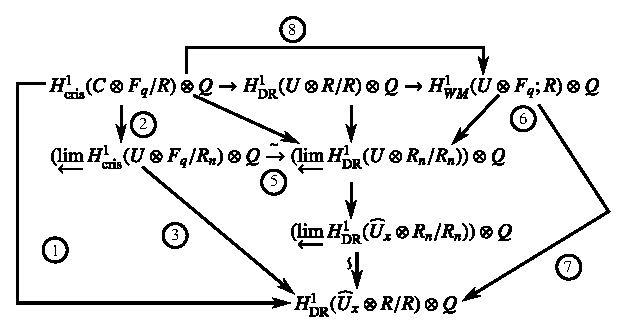
\includegraphics{chap6/fig16.eps}
\end{figure}

In\pageoriginale this diagram, the maps \mycirc{2}, \mycirc{5} and \mycirc{6} are each compatible with the actions of $F$ and of $F_{p}\times \mu_{N}$ imposed by crystalline and by $W-M$ theory (simply because these actions {\em lift} to the $U\otimes W_{n}$). Therefore the compatibility of the isomorphism \mycirc{8} with the actions of $F$ and of $F_{p}\times \mu_{N}$ would follow from the {\em injectivity} of arrows \mycirc{2} and \mycirc{6}. The injectivity of these arrows follows from the commutativity of the diagram and the already noted injectivity of arrow \mycirc{1} (which is injective exactly because $F$ has no $p$-adic unit eigenvalues in $H^{1}_{\cris}$ of our particular $C$).

\medskip
\noindent
{\bf A Question \thnum{7.8.2}.\label{art6-7.8.2}}~{\em Let $U$ be a smooth affine $W$-scheme which is the complement of a divisor with normal crossings in a proper and smooth $W$-scheme.}

{\em Are the maps}
$$
H^{1}_{\DR}(U/W)\otimes Q\to (\varprojlim H^{1}_{\DR}(U\otimes W_{n}/W_{n}))\otimes Q
$$
{\em always injective?}

\setcounter{section}{7}
\setcounter{subsection}{8}
\subsection{The Gross-Koblitz Formula}\label{art6-sec7.9}
In this section we will derive the\break Gross-Koblitz formula from our limit formulas.

Morita's $p$-adic gamma function is the unique continuous function
$$
\Gamma_{p} : Z_{p}\to Z^{\times}_{p}
$$
whose values on the strictly positive integers are given by the formula
\begin{equation*}
\Gamma_{p}(1+n)=(-1)^{n+1}\cdot \prod\limits_{\substack{1\leq i\leq n\\ p\nmid n}}i=\frac{(-1)^{n+1}\cdot n!}{[n/p]!p^{[n/p]}}\tag{7.9.1}\label{art6-eq7.9.1}
\end{equation*}
where [\quad] denotes ``integral part.''

\medskip
\noindent
{\bf Lemma \thnum{7.9.2}.\label{art6-lem7.9.2}}~{\em For any integer $n\geq 0$, and any $\pi$ satisfying $\pi^{p-1}=-p$, we have the identity}
\begin{equation*}
\frac{(-\pi)^{n}/n!}{(-\pi)^{[n/p]}/[n/p]!}=(-1)\cdot \frac{(\pi)^{n-p[n/p]}}{\Gamma_{p}(1+n)}.\tag{7.9.3}\label{art6-eq7.9.3}
\end{equation*}

\begin{proof}
This is just a rearrangement of \eqref{art6-eq7.9.1}.
\end{proof}

\medskip
\noindent
{\bf Corollary \thnum{7.9.4}.\label{art6-coro7.9.4}}~{\em Let\pageoriginale $q=p^{f}$ with $f\geq 1$, $\pi$ any solution of $\pi^{p-1}=-p$ and $n\geq 0$ any integer. Let}
$$
n=n_{0}+n_{1}p+\cdots\qquad 0\leq n_{i}\leq p-1
$$
{\em be the $p$-adic expansion of $n$. Then we have}
\begin{equation*}
\frac{(-\pi)^{n}/n!}{(-\pi)^{[n/q]}/[n/q]!}=\dfrac{(-1)^{f}\cdot (\pi)^{n_{0}+n_{1}+\cdots+n_{f-1}}}{\prod\limits^{f-1}_{i=0}\Gamma_{p}(1+[n/p^{i}])}\tag{7.9.5}\label{art6-eq7.9.5}
\end{equation*}

\begin{proof}
Simply apply \eqref{art6-eq7.9.3} successively to $n$, $[n/p],\ldots [n/p^{f-1}]$. 
\end{proof}

For a fixed integer $i\geq 0$, the map on positive integers
$$
n\mapsto [n/p^{i}]
$$
extends to a continuous function $Z_{p}\to Z_{p}$ which we denote 
$$
n\mapsto [n/p^{i}]_{p}.
$$
In terms of the $p$-adic ``digits'' of $n$, this map is just the $i$-fold shift:
\begin{equation*}
n=\sum n_{j}p^{j}\mapsto \sum\limits_{j>0}n_{j+i}p^{j}=[n/p^{i}]\tag{7.9.6}\label{art6-eq7.9.6}
\end{equation*}

\noindent
{\bf Lemma \thnum{7.9.7}.\label{art6-lem7.9.7}}~{\em Let $0<\alpha <1$ be a rational number with a prime-to-$p$ denominator. If $p^{f}=1\mod$ denom $(\alpha)$ for some $f\geq 1$, then we have the identity}
\begin{equation*}
-\langle p^{f-1}\alpha\rangle = [-\alpha/p^{i}]_{p}\quad\text{in}\quad Z\tag{7.9.8}\label{art6-eq7.9.8}
\end{equation*}
{\em for $i=0,1,\ldots,f-1$ (where $\langle\quad\rangle$ denotes the ``fractional part'' of a rational number).}

\begin{proof}
Write $(p^{f}-1)\alpha=A$. Then $A$ is an integer, $0<A<p^{f}-1$, so we may write its $p$-adic expansion as
\begin{align*}
A=a_{0}+a_{1}p+\cdots+a_{f-1}p^{f-1};\qquad & 0\leq a_{i}\leq p-1\\[3pt]
                                        & a_{i}<p-1\text{~ for {\em some~}} i.
\end{align*}

We\pageoriginale now {\em extend} the definition of $a_{n}$ to {\em all} $n\in Z$ by requiring
$$
a_{n}=a_{n+f}\qquad \forall \ n\in Z.
$$
Then
\begin{align*}
p^{f-i}\alpha=p^{f-i}\frac{A}{p^{f}-1} &= \frac{\sum\limits^{f-1}_{j=0}a_{j}p^{f+j-i}}{p^{f}-1}\\[4pt]
&\equiv \frac{\sum\limits^{f-1}_{j=0}a_{j+i}p^{j}}{p^{f}-1}\mod Z
\end{align*}
whence
\begin{align*}
-\langle p^{f-i}\alpha\rangle = \frac{\sum\limits^{f-1}_{j=0}a_{j+i}p^{j}}{1-p^{f}} &= \sum\limits_{j\geq 0}a_{j+i}p^{j}\\[4pt]
&=\left[\frac{\sum\limits_{j\geq 0}a_{j}p^{j}}{p^{i}}\right]_{p}
\end{align*}
But we readily calculate
$$
-\alpha = \frac{A}{1-p^{f}}=\sum\limits_{j\geq 0}a_{j}p^{j}.
$$
\end{proof}

\noindent
{\bf Corollary \thnum{7.9.9}.\label{art6-coro7.9.9}}~{\em Let $q=p^{f}$ with $f\geq 1$, $\pi$ any solution of $\pi^{p-1}=-p$, and $\alpha$ any rational number satisfying}
$$
\begin{cases}
0\leq \alpha \leq 1\\[3pt]
(q-1)\alpha \in Z.
\end{cases}
$$
{\em Let}
$$
A=(q-1)\alpha =a_{0}+a_{1}p+\cdots+a_{f-1}p^{f-1},\quad 0\leq a_{i}\leq p-1
$$
{\em be\pageoriginale the $p$-adic expansion of $(q-1)\alpha$, and let}
$$
S((q-1)\alpha)=a_{0}+a_{1}+\cdots+a_{f-1}
$$
{\em be the sum of the $p$-adic digits of $(q-1)\alpha$. Then we have the formula}
\begin{equation*}
\lim\limits_{n\to -\alpha}\frac{(-\pi)^{n}/n!}{(-\pi)^{[n/q]!}}=\frac{(-1)^{f}\cdot (\pi)^{S((q-1)\alpha)}}{\prod\limits^{f-1}_{i=0}\Gamma_{p}(1-\langle p^{i}\alpha\rangle )}\tag{7.9.10}\label{art6-eq7.9.10}
\end{equation*}
{\em in which the limit is taken over positive integers $n$ which approach $-\alpha$ $p$-adically.}

\begin{proof}
Simply combine \eqref{art6-eq7.9.5} and \eqref{art6-eq7.9.8}, and use the $p$-adic continuity of both $\Gamma_{p}$ and of $n\to [n/p^{i}]$.
\end{proof}

Combining this last formula with our limit formula for Gauss sums, we obtain the Gross-Koblitz formulas.

\medskip
\noindent
{\bf Theorem \thnum{7.10}\label{art6-thm7.10}}~(Gross-Koblitz).~{\em Let $N\geq 2$ prime to $p$, $E$ a number field containing the $Np$'th roots of unity, $\sfP$ a $p$-adic place of $E$, $\pi \in E_{p}$ a solution of $\pi^{p-1}=-p,\psi_{\pi}$ the corresponding additive character of $F_{p}$, a an integer $1\leq a\leq N-1$, $\chi_{a}$ the corresponding character $\zeta\mapsto \zeta^{a}$ of $\mu_{N}$, and $F_{q}$, $q=p^{f}$, a finite extension of the residue field $F_{N(\sfP)}$ of $E$ at $\sfP$. We have the formulas, in $E_{\sfP}$,}
\begin{align*}
-g_{q}(\psi_{\pi},\chi_{a};\sfP) &= \frac{(-1)^{f}\cdot q\cdot \prod\limits_{i\mod f}\Gamma_{p}\left(i-\langle \frac{p^{i}a}{N}\rangle \right)}{(\pi)^{S((q-1)\frac{a}{N})}}\tag{7.10.1}\label{art6-eq7.10.1}\\[4pt]
-g_{q}(\psi_{\pi},\overline{\chi}_{a};\sfP) &=(\pi)^{S((q-1)\frac{a}{N})}\prod\limits_{i\mod f}\Gamma_{p}\left(\langle \frac{p^{i}a}{N}\rangle\right)\tag{7.10.2}\label{art6-eq7.10.2}
\end{align*}

\begin{proof}
The sequence $n_{r}=(q^{r}-1)(a/N)$ tends to $-a/N$ as $r$ grows, and satisfies $[n_{r}/q]=n_{r-1}$ for $r\geq 1$. Therefore the first formula follows from the limit formula \eqref{art6-eq7.8.1} and from the preceding formula \eqref{art6-eq7.9.10} with $\alpha=a/N$. The second formula is obtained from the first by replacing $a$ by $N-a$.
\end{proof}

\bigskip
\noindent
{\bf VIII. Interpretation via the De Rham-Witt Complex.}\pageoriginale
Throughout this chapter, we fix an algebraically closed field $k$ of characteristic $p$, and a proper smooth connected scheme $X$ over its Witt vectors $W=W(k)$. For each $n\geq 1$, we denote by $X_{n}$ the $W_{n}$-scheme $\foprod{X}{W_{n}}{W}$.

The ``second spectral sequence'' of de Rham cohomology of $X_{n}/W_{n}$ 
$$
E^{p,q}_{2}(n)=H^{p}(X_{n},\mathscr{H}^{q}_{\DR}(X_{n}/W_{n}))\Rightarrow H^{p+q}(X_{n}/W_{n})
$$
has an intrinsic interpretation in terms of $X\otimes k$ as the Leray spectral sequence for the ``forget the thickening'' map
$$
(X\otimes k/W_{n})_{\cris}\to (X\otimes k)_{\text{Zar}}.
$$
As such, it may be rewritten
$$
E^{p,q}_{2}(n)=H^{p}(X\otimes k,\mathscr{H}^{q}_{\cris}(X\otimes k/W_{n}))\Rightarrow H^{p+q}_{\cris}(X\otimes k/W_{n}).
$$

An explicit construction of this spectral sequence may be given in terms of the De Rham-Witt pro-complex on $X\otimes k$
$$
\{W_{n}\Omega^{\bigdot}\}_{n}
$$
of Deligne and Illusie; it is simply the second spectral sequence of this complex:
$$
E^{p,q}_{2}(n)=H^{p}(X\otimes k,\mathscr{H}^{q}(W_{n}\Omega^{\bigdot}))\Rightarrow H^{p+q}(X\otimes k, W_{n}\Omega^{\bigdot}).
$$
It is known that the $E_{2}$ terms of this spectral sequence are finitely generated $W_{n}(k)$-modules. Therefore we may pass to the inverse limit and obtain a spectral sequence
$$
E^{p,q}_{2}=\varprojlim\limits_{n}E^{p,q}_{2}(n)\Rightarrow H^{p+q}_{\cris}(X\otimes k/W).
$$

Let $x$ be a $W$-valued point of $X$, and assume $X$ connected. The formal expansion map we have exploited
$$
H^{i}_{\cris}(X\otimes k/W)\simeq H^{i}_{\DR}(X/W)\to H^{i}_{\DR}(\widehat{X}_{x}/W)
$$
is the composition of the edge-homomorphism
$$
H^{i}_{\cris}(X/W)\twoheadrightarrow E^{0,i}_{\infty}\hookrightarrow E^{0,i}_{2}
$$
with the natural map
$$
E^{0,i}_{2}=\varprojlim\limits_{n}H^{0}(X_{n},\mathscr{H}^{i}_{\DR}(X_{n}/W_{n}))\to \varprojlim H^{i}_{\DR}(\widehat{X}_{x}\otimes W_{n}/W_{n}).
$$\pageoriginale

\medskip
\noindent
{\bf Lemma \thnum{8.1}.\label{art6-lem8.1}}~{\em This map is in fact injective; indeed, the induced maps}
$$
H^{0}(X_{n},\mathscr{H}^{i}_{\DR}(X_{n}/W_{n}))\to H^{i}_{\DR}(\widehat{X}_{x}\otimes W_{n}/W_{n})
$$
{\em as injective.}

\begin{proof}
Because $X_{n}$ is irreducible, it suffices to show

\smallskip
\noindent
(*) for any closed point $y$ of $X_{n}$, and any affine open $V\ni y$ which is\break \'etale over standard affine space $A=\Spec(W_{n}[T_{1},\ldots,T_{d}])$, the natural map
$$
H^{0}(V,\mathscr{H}^{i}_{\DR}(X_{n}/W_{n}))\to \mathscr{H}^{i}_{\DR}(\widehat{V}_{y}/W_{n}).
$$
is injective.

For once (*) is established we argue as follows. Let $\xi$ be a global section over $X_{n}$ of $\mathscr{H}^{i}_{\DR}$ which dies formally at $x$. We must show that for any closed point $z$ in $X_{n}$, there is an open set $V\ni z$ such that $\xi$ dies on $V$. Let $U$ be an affine open neighborhood of $x$ \'etale over $A$, and $V$ an affine open neighborhood of $z$ \'etale over $A$. Because $X_{n}$ is irreducible, $U\cap V$ is non-empty. Let $y$ be a closed point of $X_{n}$ contained in $U\cap V$.
\begin{figure}[H]
\centering
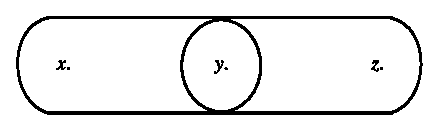
\includegraphics{chap6/fig17.eps}
\end{figure}
Then (*) for $U\ni x$ shows that $\xi$ dies on $U$. Therefore $\xi$ dies formally at $y$. Applying (*) to $V\ni y$, we find that $\xi$ dies on $V$, as required.

We now prove (*). Let $F:A\to A^{(\sigma)}$ be {\em any} $\sigma$-linear map lifting absolute Frobenius (e.g. $T_{i}\to T^{p}_{i}$). Because $V$ is \'etale over $A$, $F$ extends uniquely to a $\sigma$-linear map $F:V\to V^{(\sigma)}$ which lifts absolute Frobenius.

Because all iterates of $F$, especially $F^{n}:V\to V^{(\sigma^{n})}$, are homeomorphisms, the functor $(F^{n})_{*}$ is exact. Therefore we have
$$
\begin{cases}
H^{0}(V,\mathscr{H}^{i}_{\DR}(V/W_{n}))=H^{0}(V^{(\sigma^{n})},(F_{n})_{*}(\mathscr{H}^{i}_{\DR}(V/W_{n})))\\
(F^{n})_{*}\mathscr{H}^{i}_{\DR}(V/W_{n})=\mathscr{H}^{i}((F^{n})_{*}(\Omega^{*}_{V/W_{n}}))
\end{cases}
$$
But the complex $(F^{n})_{*}(\Omega^{\bigdot}_{V/W_{n}})$ on $V^{(\sigma^{n})}$ is a complex of locally free sheaves\pageoriginale of finite rank on $V^{(\sigma^{n})}$, with $\mathscr{O}$-linear differential. For any closed point $y \ V$, the formal stalk at $y^{(\sigma^{n})}$ is
$$
(F^{n})_{*}(\Omega^{\bigdot}_{V/W_{n}})\bigotimes\limits_{\mathscr{O}_{V^{(\sigma^{n})}}}\widehat{\mathscr{O}}_{V(\sigma^{n}),y(\sigma^{n})}\simeq (F^{n})_{*}\Omega^{\bigdot}_{\widehat{V}_{y}/W_{n}}.
$$
Therefore the sheaves on $V^{(\sigma^{n})}$
$$
\mathscr{F}^{i}=\mathfrak{F}^{i}_{V/W_{n}} {\displaystyle{\mathop{=}\limits^{\text{dfn}}}}(F^{n})_{*}(\mathscr{H}^{i}_{\DR}(V/W_{n}))=\mathscr{H}^{i}((F^{n})_{*}\Omega^{\bigdot}_{V/W_{n}})
$$
are {\em coherent}, and (by flatness of the completion) their formal stalks are given by
$$
(\widehat{\mathscr{F}}^{i})_{y^{(\sigma^{n})}}=H^{i}_{\DR}(\widehat{V}_{y}/W_{n})
$$
We must show that
$$
H^{\circ}(V^{(\sigma^{n})},\mathscr{F}^{i})\hookrightarrow (\widehat{F}^{i})_{y^{(\sigma^{n})}}.
$$
For this, it suffices to explicit a finite filtration
$$
\mathscr{F}^{i}\supset \Fil^{1}\mathscr{F}^{i}\supset \ldots
$$
whose associated graded sheaves are {\em locally free sheaves} on $V^{(\sigma^{n})}\otimes k$. We claim that the filtration induced by the $p$-adic filtration on $\Omega^{\bigdot}V/W_{n}$ has this property.

To see this, we first reduce to the case $V=A$, as follows. The diagram
\[
\xymatrix@C=2cm@R=1.5cm{
V\ar[r]^-{F^{n}}\ar[d] & V^{(\sigma^{n})}\ar[d]\\
A\ar[r]^-{F^{n}} & A^{(\sigma^{n})}
}
\]
is cartesian (because $V$ is \'etale over $A$). Therefore we have an isomorphism
$$
(F^{n})_{*}\Omega^{\bigdot}_{V/W_{n}}\xleftarrow{\sim}((F^{n})_{*}\Omega^{\bigdot}_{A/W_{n}}) \bigotimes\limits_{\mathscr{O}_{A^{(\sigma^{n})}}}\mathscr{O}_{V^{(\sigma^{n})}}.
$$
Because $\mathscr{O}_{V^{(\sigma^{n})}}$ is {\em flat} over $\mathscr{O}_{A^{(\sigma^{n})}}$, this isomorphism is a filtered isomorphism (for the $p$-adic filtrations of $\Omega^{\bigdot}_{V/W_{n}}$ and of $\Omega^{\bigdot}_{A/W_{n}}$).

By\pageoriginale flatness again, this filtered isomorphism induces isomorphisms
$$
\gr^{j}_{\Fil}(\mathscr{F}^{i}_{V/W_{n}})\simeq (\gr^{j}_{\Fil}\mathscr{F}^{i}_{A/W_{n}})\bigotimes\limits_{\mathscr{O}_{A^{(\sigma^{n})}}}\mathscr{O}_{V^{(\sigma^{n})}}
$$
It remains to show that $\gr^{j}_{\Fil}(\mathscr{F}^{i}_{A/W_{n}})$ is a locally free sheaf on $A^{(\sigma^{n})}\otimes k$. It is certainly a {\em coherent} sheaf on $A^{(\sigma^{n})}$ (because the $p$-adic filtration on $(F^{n})_{*}\Omega^{\bigdot}_{A/W_{n}}$ is $\mathscr{O}_{A^{(\sigma^{n})}}$-linear), and it is killed by $p$; therefore it is a coherent sheaf on $A^{(\sigma^{n})}\otimes k$. Because it is coherent, it is locally free on a non-void open set; if we knew that it were translation-invariant, i.e. isomorphic to all it translates by $k$-valued points of $A^{(\sigma^{n})}\otimes k$, we would conclude that it is locally free everywhere.

As a sheaf of abelian groups, it is visibly translation-invariant. It's $\mathscr{O}_{A^{(\sigma^{n})}\otimes k}$-module structure is the composite of its natural module-structure over the sheaf of rings
$$
\gr^{\circ}_{\Fil}\mathscr{H}^{\circ}_{\DR}(A/W_{n})
$$
with the $\sigma^{n}$-linear isomorphism
\begin{gather*}
\mathscr{O}_{A\otimes k}\xrightarrow{\sim} \gr^{\circ}_{\Fil}\mathscr{H}^{\circ}(A/W_{n})\\[3pt]
f\mapsto (F^{n})^{*}(\widetilde{f}),
\end{gather*}
where $\widetilde{f}$ denotes any local section of $\mathscr{O}_{A}$ lifting $f$.

To conclude the proof, we must verify that this isomorphism is translation-invariant. For this, it suffices to show that it is independent of the {\em particular choice} of $F$ lifting Frobenius which figures in its definition. For this independence, we simply notice that an ``intrinsic'' description of the same $\sigma^{n}$-linear isomorphism
$$
\mathscr{O}_{A\otimes k}\xrightarrow{\sim} \gr^{\circ}_{\Fil}\mathscr{H}^{\circ}(A/W_{n})
$$
is provided by
$$
f\mapsto (\widetilde{f})^{p^{n}}
$$
where again $\widetilde{f}\in \mathscr{O}_{A}$ denotes any lifting of $f$.
\end{proof}

\noindent
{\bf Lemma \thnum{8.2}.\label{art6-lem8.2}}~{\em The $E^{i,0}_{2}$ terms of the spectral sequence are given by}
$$
E^{i,0}_{2}\simeq H^{i}_{\et}(X\otimes k,Z_{p})\otimes W(k)
$$

\begin{proof}
For each integer $n\geq 1$, there is an isomorphism (cf. \cite{art6-key24}, \cite{art6-key25})
$$
W_{n}(O_{X\otimes k})\xrightarrow{\sim} \mathscr{H}^{0}_{\DR}(X_{n}/W_{n})
$$
defined\pageoriginale by
$$
(g_{0},\ldots,g_{n-1})\mapsto \sum\limits^{n-1}_{i=0}p^{i}(\widetilde{g}_{i})^{p^{n-i}}
$$
where $\widetilde{g}_{i}$ is a local lifting of $g_{i}\in O_{X\otimes k}$ to $O_{x_{n}}$ (Compare \eqref{art6-eq5.52}).

For variable $n$, these isomorphisms sit in a commutative diagram
\[
\xymatrix@C=1.5cm{
W_{n+r}(O_{X\otimes k})\ar@{->>}[d]^-{\text{usual projection}}\ar[r]^-{\sim} & \mathscr{H}^{0}_{\DR}(X_{n+r}/W_{n+r})\ar[dd]^-{\text{reduction mod $p^{n}$}}\\
W_{n}(O_{X\otimes k})\ar[d]^-{F^{r}} & \\
W_{n}(O_{X\otimes k})\ar[r]^-{\sim} & \mathscr{H}^{0}_{\DR}(X_{n}/W_{n}).
}
\]

Therefore we may calculate
\begin{align*}
E^{i,0}_{2} &= \varprojlim\limits_{n} H^{i}(X\otimes k, \mathscr{H}^{0}_{\DR}(X_{n}/W_{n}))\\[3pt]
          &\xrightarrow{\sim} \varprojlim\limits_{n}\left(\bigcap\limits_{r}(\text{image of~ } F^{r}\text{~ or~ } H^{i}(X\otimes k, W_{n}(O_{X\otimes k}))\right).\\[3pt]
&\simeq \varprojlim (\text{fixed points of~ } F\text{~ in~ } H^{i}(X\otimes k, W_{n}(O_{X\otimes k}))\bigotimes\limits_{Z/p^{n}Z} W_{n}(k)\\[3pt]
&\simeq \varprojlim\limits_{n} H^{i}_{\et}(X\otimes k, Z/p^{n}Z)\otimes W_{n}(k).
\end{align*}
\end{proof}

Consider now the exact sequence of terms of low degree
$$
0\to E^{1,0}_{2}\to H^{1}_{\cris}\quad (X\otimes k/W)\to E^{0,1}_{2}\xrightarrow{d_{2}}E^{2,0}_{2}
$$

\noindent
{\bf Lemma \thnum{8.3}.\label{art6-lem8.3}}~{\em The map $d^{0,1}_{2}:E^{0,1}_{2}\to E^{2,0}_{2}$ vanishes.}

\begin{proof}
Because both $H^{1}_{\cris}(X\otimes k/W)$ and $E^{2,0}_{2}=H^{2}_{\et}(X\otimes k,Z_{p})\otimes W_{j}$ are finitely generated $W$-modules, we see that $E^{0,1}_{2}$ is a finitely generated $W$-module. Therefore its inverse limit topology (as $\varprojlim E^{0,1}_{2}(n)$) is equivalent to its $p$-adic topology. Because $F^{n}$ annihilates the sheaf $\mathscr{H}^{1}_{\cris}(X\otimes k/W_{n})$, it annihilates its global sections $E^{0,1}_{2}(n)$, and hence $F$ is topologically nilpotent on $E^{0,1}_{2}$. But $F$ is an {\em automorphism} of the finitely generated $W$-module $E^{2,0}_{2}$; as $d_{2}$ commutes with $F$, this forces $d^{0,1}_{2}$ to {\em vanish}.
\end{proof}

Thus we obtain the following theorem.

\medskip
\noindent
{\bf Theorem \thnum{8.4}.\label{art6-thm8.4}}~{\em The\pageoriginale exact sequence of terms of low degree}
\[
\xymatrix@C=.75cm{
0\to H^{1}_{\et}(X\otimes k,Z_{p})\otimes \ar[r] & H^{1}_{\cris}(X\otimes k/W)\ar[d]_{\rotatebox{90}{$\sim$}}\ar[r] & E^{0,1}_{2}\ar[r]\ar@{_(->}[d] & 0\\
 & H^{1}_{\DR}(X/W)\ar[r]^-{\text{formal}}_{\text{expansion}} & H^{1}_{\DR}(\widehat{X}_{x}/W) & 
}
\]
{\em defines the Newton-Hodge filtration on $H^{1}_{\cris}$}
$$
0\to (\text{slope~}0)\to H^{1}_{\cris}(X\otimes k/W)\to (\text{slope~}>0)\to 0.
$$
[When $X/W$ is a curve, or an abelian scheme, this exact sequence coincides with the exact sequence (\eqref{art6-eq5.7.2} or \eqref{art6-thm5.9.5}!]

Illusie and Raynaud have recently been able to generalize these results to $H^{i}_{\cris}$ for all $i$. Their remarkable result is the following.

\medskip
\noindent
{\bf Theorem \thnum{8.5}.\label{art6-thm8.5}}~(Illusie-Raynaud).~{\em Let $X_{0}$ be proper and smooth over an algebraically closed field of characteristic $p>0$. The second spectral sequence of the De Rham-Witt complex}
$$
E^{p,q}_{2}=\varprojlim\limits_{n}H^{p}(X_{0},\mathscr{H}^{q}(W_{n}\Omega^{\bigdot}))\Rightarrow H^{p+q}_{\cris}(X_{0}/W)
$$
{\em degenerates at $E_{2}$ after tensoring with $Q$:}
$$
\fprod{E^{p,q}_{2}}{Q}{Z}\simeq \foprod{E^{p,q}_{\infty}}{Q}{Z}, d_{r}\otimes Q=0\text{~~ for~~ } r\geq 2,
$$
{\em and defines the Newton-Hodge filtration on $H_{\cris}(X_{0}/W)\otimes Q$:}
$$
q-1<\text{slopes of~}E^{p,q}_{2}\otimes Q\leq q.
$$

\smallskip
\noindent
{\bf Corollary \thnum{8.6}.\label{art6-coro8.6}}~{\em If $X_{0}/k$ lifts to $X/W$, then for any $W$-valued point $x$ of $X$, and any integer $i$, the image of the formal expansion map}
$$
H^{i}_{\cris}(X\otimes k/W)\otimes Q\simeq H^{i}_{\DR}(X/W)\otimes Q\to H^{i}_{\DR}(\widehat{X}_{x}/W)\otimes Q
$$
{\em is precisely the quotient ``slopes $>i-1$'' of $H^{i}_{\cris}\otimes Q$.}

\begin{thebibliography}{99}
\bibitem{art6-key1} \textsc{Atkin,}\pageoriginale A. O. L. and P. H. F. \textsc{Swinnerton-Dyer,} : Modular forms on non-congruence subgroups. {\em Proc. Symposia Pure Math} XIX, 1--25, A. M. S. (1971).

\bibitem{art6-key2} \textsc{Berthelot,} P. : {\em Cohomologie Cristalline des Sch\'emas de Caracteristique} $p>0$. Springer Lecture Notes in Math 407, Springer-Verlag (1974).

\bibitem{art6-key3} \textsc{Berthelot,} P. and A. Ogus, : {\em Notes on Crystalline Cohomology}. Princeton University Press (1978).

\bibitem{art6-key4} \textsc{Bloch,} S. : Algebraic $K$-theory and crystalline cohomology. {\em Pub. Math. I. H. E. S.} 47, 187--268 (1978).

\bibitem{art6-key5} \textsc{Cartier,} P. : Groupes formels, fonctions automorphes et fonctions zeta des courbes elliptiques, {\em Actes, 1970 Congr\'es Intern. Math.} Tome 2, 291--299 (1971).

\bibitem{art6-key6} \textsc{Deligne,} P. : La conjecture de Weil I {\em Pub. Math. I. H. E. S.} 43, 273--307 (1974).

\bibitem{art6-key7} ---------- : Sommes trigonometriques, S. G. A. $4\frac{1}{2}$, {\em Cohomologie Etale}. Springer Lecture Notes in Math 569, Springer Verlag (1977).

\bibitem{art6-key8} \textsc{Ditters,} B. : {\em On the congruences of Atkin and Swinnerton-Dyer}. Report 7610, February 1976, Math Inst. Kath. Unis, Nijmegen, Netherlands (preprint).

\bibitem{art6-key9} \textsc{Dwork,} B. : On the zeta function of a hypersurface. {\em Pub. Math. I. H. E. S.} 12 (1962).

\bibitem{art6-key10} ---------- : On the zeta function of a hypersurface II. {\em Ann. Math.} (2) (80), 227--299 (1964).

\bibitem{art6-key11} ---------- : Bessel functions as $p$-adic functions of the argument. {\em Duke Math. J.} vol. 41, no. 4, 711--738 (1974).

\bibitem{art6-key12} \textsc{M. Boyarsky,} : $P$-adic gamma functions and Dwork cohomology, to appear in {\em T. A. M. S.}

\bibitem{art6-key13} \textsc{Fontaine,} J.-M. : {\em Groupes $p$-divisibles sur les corps locaux}. Asterisque 47--48, Soc. Math. France (1977).

\bibitem{art6-key14} \textsc{Gross,} B. H. and N. Koblitz, : Gauss sums and the $p$-adic $\Gamma$-functions. {\em Ann. Math.} vol. 109, no. 3 (1979).

\bibitem{art6-key15} \textsc{Gross,} B. H. : On the periods of abelian integrals and a formula of Chowla-Selberg, with an appendix by David Rohrlich. {\em Inv. Math.} 45, 193--211 (1978).

\bibitem{art6-key16} \textsc{Grothendieck,} A. : {\em Rev\'etements Etales et Groupe Fondamental (SGA 1).} Springer Lecture Notes in Math. 244, Springer-Verlag (1971).

\bibitem{art6-key17} ---------- :\pageoriginale Groupes de Barsotti-Tate et Cristaux. {\em Actes du Cong. Intern. Math.} 1970, tome 1, 431--436 (1971).

\bibitem[17 bis.]{art6-key17bis} ---------- : Groupes de Barsotti-Tate et cristaux de Dieudonn\'e. {\em Sem. Math. Sup.} 45, Presses Univ. de Montr\'eal (1970).

\bibitem{art6-key18} ---------- : Formule de Lefschetz et rationalit\'e des fonctions L. {\em Expos\'e 279, Seminaire Bourbaki} 1964/65.

\bibitem{art6-key19} \textsc{Hartshorne,} R. : On the de Rham cohomology of algebraic varieties. {\em Pub. Math. I. H. E. S.} 45, 5--99 (1976).

\bibitem{art6-key20} \textsc{Hasse,} H. : Theorie der relativ-zyklischen algebraischen Funktionenk\"orp\'er, insbesondere bei endlichem Konstantenk\"orp\'er. {\em J. Reine Angew. Math.} 172, 37--54 (1934).

\bibitem{art6-key21} ---------- and H. \textsc{Davenport} : Die Nullstellen der Kongruenz zeta-funktionen in gewissen zyklischen F\"allen. {\em J. Reine Angew. Math.} 172, 151--182. (1934).

\bibitem{art6-key22} \textsc{Honda}, T. : On the theory of commutative formal groups. {\em J. Math. Soc. Japan,} 22, 213--246 (1970).

\bibitem{art6-key23} ---------- : On the formal structure of the Jacobian variety of the Fermat curve over a $p$-adic integer ring. {\em Symposia Matematica} XI, Istituto Nazionale Di Alta Matematica, 271--284, Academic Press (1973).

\bibitem{art6-key24} \textsc{Illusie,} L. : Complex de DeRham-Witt et cohomologie cristalline. to appear.

\bibitem{art6-key25} ---------- : Complex de DeRham-Witt. {\em Proceedings of the 1978 Journe\'es de G\'eom\'etrie Algebriques de Renn\'es,} to appear in Asterisque.

\bibitem{art6-key26} ---------- and M. \textsc{Raynaud,} : work in preparation.

\bibitem{art6-key27} \textsc{Katz,} N. : Nilpotent connections and the monodromy theorem. {\em Pub. Math. I. H. E. S.} 39, 175--232 (1970).

\bibitem{art6-key28} ---------- : {\em $P$-adic properties of modular schemes and modular forms.} Proc. 1972 Antwerp Summer School, Springer Lecture Notes in Math 350, 70--189 (1973).

\bibitem{art6-key29} ---------- and W. \textsc{Messing}, : Some consequences of the Riemann hypothesis for varieties over finite fields. {\em Inv. Math.} 23, 73--77 (1974).

\bibitem{art6-key30} ---------- : {\em Slope filtration of $F$-crystals}. Proceedings of the 1978 Journe\'es de G\'eom\'etrie Alg\'ebrique de Rennes, to appear in Asterisque.

\bibitem{art6-key31} \textsc{Koblitz,} N. : {\em A short course on some current research in $p$-adic analysis}. Hanoi, 1978, preprint.

\bibitem{art6-key32} \textsc{Lang,} S. : {\em Cyclotomic Fields II.} Springer Verlag.

\bibitem{art6-key33} \textsc{Lazard,} M. : Lois\pageoriginale de groupes et analyseurs. {\em Ann. Sci. Ec. Norm. Sup. Paris} 72, 299-400 (1955).

\bibitem{art6-key34} ---------- : {\em Commutative Formal Groupes.} Springer Lecture Notes in Math. 443, Springer-Verlag (1975).

\bibitem{art6-key35} \textsc{Mazur,} B. and W. \textsc{Messing,} : {\em Universal Extensions and One-Dimensional Crystalline Cohomology.} Springer Lecture Notes in Math. 370, Springer-Verlag (1974).

\bibitem{art6-key36} \textsc{Messing,} W. : {\em The Crystals Associated to Barsotti-Tate Groups.} Springer Lecture Notes in Math 264, Springer-Verlag (1972).

\bibitem{art6-key37} --------- : The universal extension of an Abelian variety by a vector group. {\em Symposia Matematica} XI, Istituto Nazionale Di Alta Matematica 358--372, Academic Press (1973).

\bibitem{art6-key38} \textsc{Monsky,} P. : {\em $P$-adic analysis and zeta functions.} Lectures at Kyoto University, Kinokuniya Book Store, Tokyo or Brandeis Univ. Math. Dept. (1970).

\bibitem{art6-key39} ---------- and G. \textsc{Washnitzer,} : Formal Cohomology I. {\em Ann. Math.} 88, 181--217 (1968).

\bibitem{art6-key40} ---------- : One-dimensional formal cohomology, {\em Actes, 1970 Congr\'es Intern. Math.} Tome 1, 451--456 (1971).

\bibitem{art6-key41} \textsc{Morita,} Y. : A $p$-adic analogue of the $\Gamma$-function. {\em J. Fac. Sci. Univ.} Tokyo 22, 255-266 (1975).

\bibitem{art6-key42} \textsc{Mumford} D. : {\em Geometric Invariant Theory.} Springer-Verlag (1965).

\bibitem{art6-key43} ---------- : {\em Abelian Varieties.} Oxford Univ. Press (1970).

\bibitem{art6-key44} \textsc{Ida,} T. : The first de Rham cohomology group and Dieudonn\'e modules. {\em Ann. Sci. Ec. Norm. Sup. Paris,} 3i\'eme serie, Tome 2, 63--135 (1969).

\bibitem{art6-key45} \textsc{Serre,} J.-P. : {\em Groupes Alg\'ebrtiques et Corps de Classes.} esp. Chapt VII, Hermann (1959).

\bibitem{art6-key46} \textsc{Weil,} A. : On some exponential sums. {\em Proc. Nat. Acad. Sci: U.S.A.} 34, 204--207 (1948).

\bibitem{art6-key47} ---------- : Number of solutions of equations in finite fields. {\em Bull. A. M. S.} 497--508 (1949).

\bibitem{art6-key48} ---------- : Jacobi sums as Gr\"ossencharaktere. {\em Trans. A. M. S.} 73, 487--495 (1952).

\end{thebibliography}
